% ***************************************************************************************************
%
%	Szablon pracy magisterskiej dla Politechniki Wrocławskiej w wersji dwustronnej.
%	Autor:	Tomasz Strzałka
%
% ***************************************************************************************************




% Styl dwustronny z domyślną wielkością czcionki 10pt oraz oddzieloną stroną tytułową (titlepage).
% Domyślnie rodziały rozpoczynają się na stronie prawej (openright).
\documentclass[]{book}



% ***************************************************************************************************
% Ustawienia języka																					*
% ***************************************************************************************************




% Podstawowe ustawienia języka, według którego formatowany będzie dokument
\usepackage[polish]{babel}


% Pakiet babel dla polskiego języka powoduje konflikt z pakietem amssymb.
% Polecenie '\lll' definiują oba pakiety - porządana jest druga definicja.
\let\lll\undefined


% W przypadku wielojęzykowości ustawia główny język dokumentu
\selectlanguage{polish}


% Kodowanie dokumentu
\usepackage[utf8]{inputenc}


% Dowolny rozmiar czcionek, kodowanie znaków
\usepackage{lmodern}


% Polskie wcięcia akapitów
\usepackage{indentfirst}


% Polskie łamanie wyrazów
\usepackage{polski}


% Przecinek w wyrażeniach matematycznych zamiast kropki
\usepackage{icomma}


% Polskie formatowanie typograficzne
\frenchspacing


% Zapewnia liczne usprawnienia wyświetlania i organizacji matematycznych formuł. 
\usepackage{amsmath}


% Wprowadza rozszerzony zestaw symboli m.in. \leadsto
\usepackage{amssymb}


% Dodatkowa, ,,kręcona'' czcionka matematyczna
\usepackage{mathrsfs}


% Dodatkowe wsparcie dla środowiska mathbb, które nie wspiera domyślnie cyfr (\mathbbm{})
\usepackage{bbm}


% Fixes/improves amsmath
\usepackage{mathtools}




% ***************************************************************************************************
% Kolory																							*
% ***************************************************************************************************




% Umożliwia rozszerzoną kontrolę nad kolorami.
\usepackage{xcolor}


% Definicje kolorów
\definecolor{lgray}{HTML}{CCCCCC}
% lgray				-	nazwa nowo zdefiniowanego koloru
% HTML				-	model kolorów
% CCCCCC			-	wartość koloru zgodna z modelem


% Kolory specyficzne dla kolorowania składni języka C/C++
\colorlet{blueC}{green!40!black}
% blueC				-	nazwa nowego koloru
% green!40!black	-	wymieszanie kolorów: 40% zielonego i 60% czarnego


\colorlet{greenC}{purple!40!black}
% greenC			-	nazwa nowego koloru
% purple!40!black	-	wymieszanie kolorów w stosunku 4:6




% ***************************************************************************************************
% Algorytmy																							*
% ***************************************************************************************************




% Udostępnia środowisko do konstruowania pseudokodów
\usepackage[ruled,vlined,linesnumbered,longend]{algorithm2e}
% ruled				-	poziome kreski na początku i końcu algorytmu, podpis na górze oddzielony również kreską poziomą
% vlined			-	pionowe kreski łączące początek polecenia z jego końcem
% linesnumbered		-	numerowanie kolejnych wierszy algorytmu
% longend			-	długie końcówki np. ifend, forend itd.


% Zamiana nazwy środowiska z domyślnej "Algorithm X" na "Pseudokod X"
\newenvironment{pseudokod}[1][htb]{
	\renewcommand{\algorithmcfname}{Pseudokod}
	\begin{algorithm}[#1]%
}{
	\end{algorithm}
}


% Zdefiniowanie słów kluczowych
\newcommand\KwTrue[0]{
	\emph{\textbf{TRUE}}
}


\newcommand\KwFalse[0]{
	\emph{\textbf{FALSE}}
}


\newcommand\KwNull[0]{
	\emph{\textbf{NULL}}
}


% Zmiana rozmiaru komentarzy
\newcommand\algcomment[1]{
	\footnotesize{#1}
}


% Ustawienie zadanego stylu dla komentarzy
\SetCommentSty{algcomment}


% Listowanie kodów źródłowych (C, bash, perl)
\usepackage{listings} 


% Styl wyświetlania listingów dla języka C
\lstdefinestyle{customc}{
	breaklines		=	true,					% Automatyczne łamanie linii
	xleftmargin		=	\leftmargin,			% Wyrównanie listingu do marginesu
	language		=	C,						% Język kodu źródłowego
	showstringspaces=	false,					% Pokazywanie białych znaków
	basicstyle		=	\footnotesize\ttfamily,	% Rozmiar czcionki
	keywordstyle	=	\bfseries\color{blueC},	% Definicje stylów: słów kluczowych
	commentstyle	=	\itshape\color{greenC},	% komentarzy
	identifierstyle	=	\color{blue},			% identyfikatorów
	stringstyle		=	\color{orange}			% łańcuchów znaków
}


% Definicje pecjalnych znaków, które nie są obsługiwane w środowisku listing
\lstset{literate=
	{ż}{{\.{z}}}1	{ź}{{\'{z}}}1
	{ć}{{\'{c}}}1	{ń}{{\'{n}}}1
	{ą}{{\c a}}1	{ś}{{\'{s}}}1
	{ł}{{\l}}1		{ę}{{\c{e}}}1
	{ó}{{\'{o}}}1	{á}{{\'a}}1
	{é}{{\'e}}1		{í}{{\'i}}1
	{ó}{{\'o}}1		{ú}{{\'u}}1
	{ù}{{\`u}}1		{Á}{{\'A}}1
	{É}{{\'E}}1		{Í}{{\'I}}1
	{Ó}{{\'O}}1		{Ú}{{\'U}}1
	{à}{{\`a}}1		{è}{{\'e}}1
	{ì}{{\`i}}1		{ò}{{\`o}}1
	{ò}{{\`o}}1		{À}{{\`A}}1
	{È}{{\'E}}1		{Ì}{{\`I}}1
	{Ò}{{\`O}}1		{Ò}{{\`O}}1
	{ä}{{\"a}}1		{ë}{{\"e}}1
	{ï}{{\"i}}1		{ö}{{\"o}}1
	{ü}{{\"u}}1		{Ä}{{\"A}}1
	{Ë}{{\"E}}1		{Ï}{{\"I}}1
	{Ö}{{\"O}}1		{Ü}{{\"U}}1
	{â}{{\^a}}1		{ê}{{\^e}}1
	{î}{{\^i}}1		{ô}{{\^o}}1
	{û}{{\^u}}1		{Â}{{\^A}}1
	{Ê}{{\^E}}1		{Î}{{\^I}}1
	{Ô}{{\^O}}1		{Û}{{\^U}}1
	{œ}{{\oe}}1		{Œ}{{\OE}}1
	{æ}{{\ae}}1		{Æ}{{\AE}}1
	{ß}{{\ss}}1		{ç}{{\c c}}1
	{Ç}{{\c C}}1	{ø}{{\o}}1
	{å}{{\r a}}1	{Å}{{\r A}}1
	{€}{{\EUR}}1	{£}{{\pounds}}1
}




% ***************************************************************************************************
% Marginesy																							*
% ***************************************************************************************************




% Ustawienia rozmiarów stron i ich marginesów
\usepackage[headheight=14pt, top=25mm, bottom=25mm, left=25mm, right=25mm]{geometry}
% headheight		-	wysokość tytułów
% top				-	margines górny
% bottom			-	margines dolny
% left				-	margines lewy
% right				-	margines prawy


% Usunięcie górnego marginesu dla środowisk
\makeatletter
	\setlength\@fptop{0\p@}	
\makeatother




% ***************************************************************************************************
% Styl																								*
% ***************************************************************************************************




% Definiuje środowisko 'titlingpage', które zapewnia pełną kontrolę nad układem strony tytułowej.
\usepackage{titling}


% Umożliwia modyfikowanie stylu spisu treści
\usepackage{tocloft}	


\tocloftpagestyle{tableOfContentStyle}


% Definiowanie własnych stylów nagłówków i/lub stopek
\usepackage{fancyhdr}


% Domyślny styl dla pracy 
\fancypagestyle{custom}{
	\fancyhf{}									% wyczyść stopki i nagłówki
	\fancyhead[RO]{								% Prawy, nieparzysty nagłówek
		\hrulefill \hspace{16pt} \large Rozdział \thechapter
		\put(-472.1, 12.1){%
			\makebox(0,0)[l]{%
				
\includegraphics[width=0.05\textwidth]{pwr-logo}
			}
		}
		\put(-443,5.5){%
			\makebox(0,0)[l]{%
				\small Politechnika Wrocławska
			}
		}
	}
	\fancyhead[LE]{								% Lewy, parzysty nagłówek
		\large Rozdział \thechapter \hspace{16pt} \hrulefill 
		\put(-22, 12.1){%
			\makebox(0,0)[l]{%
				
\includegraphics[width=0.05\textwidth]{wppt-logo}
			}
		}
		\put(-210,5.5){%
			\makebox(0,0)[l]{%
				\small Wydział Podstawowych Problemów Techniki
			}
		}
	}
	\fancyfoot[LE,RO]{							% Stopki
		\thepage
	}
	\renewcommand{\headrulewidth}{0pt}			% Grubość linii w nagłówku
	\renewcommand{\footrulewidth}{0.2pt}		% Grubość linii w stopce
}


% Domyślny styl dla dodatków
\fancypagestyle{appendixStyle}{
	\fancyhf{}									% wyczyść stopki i nagłówki
	\fancyhead[RO]{								% Prawy, nieparzysty nagłówek
		\hrulefill \hspace{16pt} \large Dodatek \thechapter
		\put(-472.1, 12.1){%
			\makebox(0,0)[l]{%
				
\includegraphics[width=0.05\textwidth]{pwr-logo}
			}
		}
		\put(-443,5.5){%
			\makebox(0,0)[l]{%
				\small Politechnika Wrocławska
			}
		}
	}
	\fancyhead[LE]{								% Lewy, parzysty nagłówek
		\large Dodatek \thechapter \hspace{16pt} \hrulefill 
		\put(-22, 12.1){%
			\makebox(0,0)[l]{%
				
\includegraphics[width=0.05\textwidth]{wppt-logo}
			}
		}
		\put(-210,5.5){%
			\makebox(0,0)[l]{%
				\small Wydział Podstawowych Problemów Techniki
			}
		}
	}
	\fancyfoot[LE,RO]{							% Stopki
		\thepage
	}
	\renewcommand{\headrulewidth}{0pt}			% Grubość linii w nagłówku
	\renewcommand{\footrulewidth}{0.2pt}		% Grubość linii w stopce
}


% Osobny styl dla stron zaczynających rozdział/spis treści itd. (domyślnie formatowane jako "plain")
\fancypagestyle{chapterBeginStyle}{
	\fancyhf{}%
	\fancyfoot[LE,RO]{
		\thepage
	}
	\renewcommand{\headrulewidth}{0pt}
	\renewcommand{\footrulewidth}{0.2pt}
}


% Styl dla pozostałych stron spisu treści
\fancypagestyle{tableOfContentStyle}{
	\fancyhf{}%
	\fancyfoot[LE,RO]{
		\thepage
	}
	\renewcommand{\headrulewidth}{0pt}
	\renewcommand{\footrulewidth}{0.2pt}
}


% Formatowanie tytułów rozdziałów i/lub sekcji
\usepackage{titlesec}


% Formatowanie tytułów rozdziałów
\titleformat{\chapter}[hang]					% kształt
{
	\vspace{-10ex}
	\Huge
	\bfseries
}												% formatowanie tekstu modyfikowanego elementu
{}												% etykieta występująca przed tekstem modyfikowanego elementu, niewidoczna w spisie treści
{
	10pt
}												% odstęp formatowanego tytułu od lewego marginesu/etykiety
{
	\Huge
	\bfseries
}												% formatowanie elementów przed modyfikowanym tytułem
[
	\vspace{2ex}
	\rule{\textwidth}{0.4pt}
	\vspace{-4ex}
]												% dodatkowe formatowanie stosowane poniżej modyfikowanego tytułu


% Formatowanie tytułów sekcji
\titleformat{\section}[hang]					% kształt
{
	\vspace{2ex}
	\titlerule\vspace{1ex}
	\Large\bfseries
}												% formatowanie tekstu modyfikowanego elementu
{
	\thesection									% etykieta występująca przed tekstem modyfikowanego elementu, niewidoczna w spisie treści
}
{
	0pt
}												% odstęp formatowanego tytułu od lewego marginesu/etykiety
{
	\Large
	\bfseries
}												% formatowanie elementów przed modyfikowanym tytułem




% ***************************************************************************************************
% Linki																								*
% ***************************************************************************************************




% Umożliwia wstawianie hiperłączy do dokumentu
\usepackage[draft]{hyperref}					% Wyłączenie linków (pewna wersja do druku)
%\usepackage{hyperref}							% Aktywuje linki


\hypersetup{
	ocgcolorlinks	=	true,					% Wyłącza kolorowanie linków w czasie druku (eksperymentalnie).
	colorlinks		=	true,					% Koloruje tekst zamiast tworzyć ramki.
	linkcolor		=	blue,					% Kolory: referencji,
	filecolor		=	magenta,				% łączy do plików,
	urlcolor		=	cyan					% hiperlinków.
}
 
 
% Do stworzenia hiperłączy zostanie użyta ta sama (same) czcionka co dla reszty dokumentu
\urlstyle{same}




% ***************************************************************************************************
% Listy																								*
% ***************************************************************************************************




% Umożliwia zdefiniowanie własnego stylu wyliczeniowego
\usepackage{enumitem}


% Nowa lista numerowana z trzema poziomami
\newlist{myitemize}{itemize}{3}


% Definicja wyglądu znacznika pierwszego poziomu
\setlist[myitemize,1]{
	label		=	\textbullet,
	leftmargin	=	4mm}


% Definicja wyglądu znacznika drugiego poziomu
\setlist[myitemize,2]{
	label		=	$\diamond$,
	leftmargin	=	8mm}


% Definicja wyglądu znacznika trzeciego poziomu
\setlist[myitemize,3]{
	label		=	$\diamond$,
	leftmargin	=	12mm
}




% ***************************************************************************************************
% Inne pakiety																						*
% ***************************************************************************************************




% Dołączanie rysunków
\usepackage{graphicx}


% Figury i przypisy
\usepackage{caption}


\usepackage{subcaption}


% Umożliwia tworzenie przypisów wewnątrz środowisk
\usepackage{footnote}


% Umożliwia tworzenie struktur katalogów
\usepackage{dirtree}


% Rozciąganie komórek tabeli na wiele wierszy
\usepackage{multirow}


% Precyzyjne obliczenia szerokości/wysokości dowolnego fragmentu wygenerowanego przez LaTeX
\usepackage{calc}




% ***************************************************************************************************
% Matematyczne skróty																				*
% ***************************************************************************************************




% Skrócony symbol liczb rzeczywistych
\newcommand{\RR}{\mathbb{R}}


% Skrócony symbol liczb naturalnych
\newcommand{\NN}{\mathbb{N}}


% Skrócony symbol liczb wymiernych
\newcommand{\QQ}{\mathbb{Q}}


% Skrócony symbol liczb całkowitych
\newcommand{\ZZ}{\mathbb{Z}}


% Skrócony symbol logicznej implikacji
\newcommand{\IMP}{\rightarrow}


% Skrócony symbol  logicznej równoważności
\newcommand{\IFF}{\leftrightarrow}




% ***************************************************************************************************
% Środowiska																						*
% ***************************************************************************************************




% Środowisko do twierdzeń
\newtheorem{theorem}{Twierdzenie}[section]


% Środowisko do lematów
\newtheorem{lemma}{Lemat}[section]


% Środowisko do przykładów
\newtheorem{example}{Przykład}[section]


% Środowisko do wniosków
\newtheorem{corollary}{Wniosek}[section]


% Środowisko do definicji
\newtheorem{definition}{Definicja}[section]


% Środowisko do dowodów
\newenvironment{proof}{
	\par\noindent \textbf{Dowód.}
}{
	\begin{flushright}
		\vspace*{-6mm}\mbox{$\blacklozenge$}
	\end{flushright}
}


% Środowisko do uwag
\newenvironment{remark}{
	\bigskip \par\noindent \small \textbf{Uwaga.}
}{
	\begin{small}
		\vspace*{4mm}
	\end{small}
}




% ***************************************************************************************************
% Słownik																							*
% ***************************************************************************************************




% Prawidłowe dzielenie wyrazów
\hyphenation{wszy-stkich ko-lu-mnę każ-da od-leg-łość
   dzie-dzi-ny dzie-dzi-na rów-nych rów-ny
   pole-ga zmie-nna pa-ra-met-rów wzo-rem po-cho-dzi
   o-trzy-ma wte-dy wa-run-ko-wych lo-gicz-nie
   skreś-la-na skreś-la-ną cał-ko-wi-tych wzo-rów po-rzą-dek po-rząd-kiem
   przy-kład pod-zbio-rów po-mię-dzy re-pre-zen-to-wa-ne
   rów-no-waż-ne bi-blio-te-kach wy-pro-wa-dza ma-te-ria-łów
   prze-ka-za-nym skoń-czo-nym moż-esz na-tu-ral-na cią-gu tab-li-cy
   prze-ka-za-nej od-po-wied-nio}




% ***************************************************************************************************
% Dokument																							*
% ***************************************************************************************************




\frontmatter

\begin{document}

	\begin{titlingpage}
		\vspace*{\fill}
		\begin{center}
			\begin{picture}(300,510)
				\put(11,520){\makebox(0,0)[l]{\large \textsc{Wydział Podstawowych Problemów Techniki}}}
				\put(11,500){\makebox(0,0)[l]{\large \textsc{Politechniki Wrocławskiej}}}
				\put(28,360){\Huge \textsc{Wybrane problemy}}
				\put(-75,320){\Huge \textsc{odpornej optymalizacji dyskretnej}}
				\put(-16,280){\Huge \textsc{z możliwością modyfikacji}}
				\put(97,240){\makebox(0,0)[l]{\large \textsc{Tomasz Strzałka}}}
				\put(200,100){\makebox(0,0)[l]{\large Praca magisterska napisana}}
				\put(200,80){\makebox(0,0)[l]{\large pod kierunkiem}}
				\put(200,60){\makebox(0,0)[l]{\large dr hab. Pawła Zielińskiego, prof. PWr}}
				
				\put(115,-70){
\includegraphics[width=0.15\textwidth]{pwr}}
				\put(106,-80){\makebox(0,0)[bl]{\large \textsc{Wrocław 2016}}}
			\end{picture}
		\end{center}	
		\vspace*{\fill}
	\end{titlingpage}
	
	\mbox{}
	\thispagestyle{empty}
	\newpage
	
	\begin{titlingpage}
		\vspace*{\fill}
		\begin{center}
			\begin{picture}(300,510)
				\put(100, 130){\makebox(0,0)[l]{Podziękowania chciałbym skierować do mojego promotora,}}
				\put(100, 115){\makebox(0,0)[l]{dr hab. Pawła Zielińskiego, prof. nadzw. Politechniki Wrocławskiej,}}
				\put(100, 100){\makebox(0,0)[l]{za nakład włożonej pracy w~korektę tekstu,}}
				\put(100, 85){\makebox(0,0)[l]{poświęcony na konsultacjach czas oraz zaangażowanie,}}
				\put(100, 70){\makebox(0,0)[l]{płynące z~chęci pomocy w~przygotowaniu jak najlepszej pracy dyplomowej.}}
				\put(100, 45){\makebox(0,0)[l]{X,}}
				\put(100, 30){\makebox(0,0)[l]{X}}
				\put(100, 15){\makebox(0,0)[l]{X}}
				\put(100, 0){\makebox(0,0)[l]{X.}}
				\put(-90,-100){
\includegraphics[width=0.1\textwidth]{pwr}}
			\end{picture}
		\end{center}
		\vspace*{\fill}
	\end{titlingpage}
	
	\mbox{}
	\thispagestyle{empty}
	\newpage
	
	\pagenumbering{Roman}
	\pagestyle{tableOfContentStyle}
	\tableofcontents
	\cleardoublepage
	
	\mbox{}
	\thispagestyle{empty}
	\newpage
	
	\mbox{}
	\thispagestyle{empty}
	\newpage
	
	
	
	
	% ***************************************************************************************************
	% Wstęp																								*
	% ***************************************************************************************************
	
	
	\pagestyle{custom}
	\mainmatter
	
	\clearpage
	\chapter{Wstęp}
\thispagestyle{chapterBeginStyle}


Przed skorzystaniem z dokumentu zalecam zapoznać się z szablonem pracy dyplomowej \href{http://prac.im.pwr.wroc.pl/~cichon/MaterialyDydaktyczne/PracDypl.zip}{,,WzorPracy.tex''}, znajdującego się na \href{http://prac.im.pwr.wroc.pl/~cichon/thesis.php}{stronie} prof. dr hab. Jacka Cichonia, gdyż choć niektóre zawarte w nim sformułowania wydają się bardziej niż oczywiste, warto je przyswoić.

Wartym podkreślenia jest fakt, że niniejszy szablon pracy dyplomowej powstał właśnie w oparciu o powyższy dokument, znacznie go rozbudowując.

Zawierające wspomniany plik archiwum \href{SzablonPracy.zip}{,,SzablonPracy.zip''}, powinno być dołączone do niniejszego dokumentu.
W przypadku jego braku należy pobrać je z podanej na wstępie strony.

Treść właściwego dokumentu jest jedynie uzupełnieniem podstawowych informacji zawartych w dokumencie \href{http://prac.im.pwr.wroc.pl/~cichon/MaterialyDydaktyczne/PracDypl.zip}{,,WzorPracy.tex''} i skupia się głównie na sposobie wykorzystania dodatkowych pakietów, sugerując przy okazji trzymanie się jednego, konkretnego stylu pisania.
	\clearpage
	
	
	
	
	% ***************************************************************************************************
	% Rodziały																							*
	% ***************************************************************************************************
	
	
	
	
	\clearpage
	\chapter{Min–max and min–max regret versions of combinatorial optimization problems: A survey}
\thispagestyle{chapterBeginStyle}


\begin{itemize}
	\item Paramatry (współczynniki) funkcji celu mogą być niepewne, podchodzimy do tego problemu z pomysłem scenariuszy: albo dyskretnych albo ciągłych (interval scenario case) na przedziałach, gdzie każdy parametr jest określony przez LB i UB.
	\item Mamy dwa główne modele: ostrożnej |(min-maxowej optymalizacji) i ostrożnej optymalizacji z kryterium żalu (regret criterion):
	\begin{itemize}
		\item W przypadku dyskretnym mamy $|S| = m$ scenariuszy $s$, każdy jest reprezentowany wektorem współczynników funkcji celu $c^{s} = (c_1^s , ... c_n^s)$, gdzie każdy współczynnik jest naturalny (w przypadku problemu 0-1) $\forall s \in S c_i^s \in N, i \in 1, ..., n$.
		\item W przypadku scenariuszy ciągłych (opartych na przedziałach) każdy współczynnik $c_i$ może przyjąć wartość z przedziału $[\underline{x_i}, \overline{c_i}]$, gdzie $ 0 \leqslant \underline{c_i} \leqslant \overline{c_i}$ a zbiór scenariuszy jest produktem kartezjańskim wszystkich z nich.
		\item Ekstremalne (krytyczne) scenariusze (extreme scenario) to oczywiście: $\underline{s} = ( \underline{c_1}, ..., \underline{c_n})$ i $\overline{s}$, gdzie dla każdego $i \in 1, ..., n$ $c_i = \overline{c_i}$.
		\item $c_s(x)$ --- wartość rozwiązania dla wektora zmiennych decyzyjnych $x \in X$ dla danego scenariusza $s \in S$.
		\item $c_s^\ast$ --- wartość optymalnego rozwiązania dla danego scenariusza $s$.
		\item $x^\ast_{\left( s \right)}$ --- wektor wartości zmiennych decyzyjnych dla optymalnego rozwiązania dla scenariusza $s$ i ${c_s^\ast} = c_s(x^\ast_{\left( s \right)})$.
		\item W pierwszym przypadku dla dyskretnych scenariuszy po prostu liczymy każdy scenariusz i wybieramy takie rozwiązanie, które da nam minimalną wartość dla najgorszego z możliwych scenariuszy spośród optymalnych rozwiązań ($c(x^\ast) = \min_{x \in X} max_{s \in S} c_{s}(x)$). Bez optymalizacji musimy wziąć każde możliwe rozwiązanie $x \in X$, wyliczyć dla wszystkich sceniariuszy $s \in S$ wartości $c_s(x)$, wybrać z tak powstałych grup ($C_S^x = (c_{s_1}(x), ..., c_{s_m}(x))$ - $m$ scenariuszy) max i z tak powstałej grupy: $C_X^{max} = (\max{C_S^{x_1}}, ..., \max{C_S^{x_{2^k}}})$ ($k$ binarnych zmiennych decyzyjnych dla problemu $\mathscr{P} \in \mathscr{C}$) wybrać taki $x \in X$, że $c(x) = \min{C_X^{max}}$. Czyli po polsku liczymy dla wszystkich możliwych $x \in X$ dla którego scenariusza $s \in S$ $c_s(x)$ osiągnie największą wartość a potem wybieramy takiego $x$, dla którego ta wartość maksymalna jest najmniejsza spośród pozostałych. Czyli chcemy zminimalizować straty w najbardziej pesymistycznym przypadku
		\item W przypadku min-max regret criteria nie chcemy minimalizować strat bez względu na dziejący się sceiariusz, lecz jesteśmy zainteresowani wyborem takiego rozwiązania, które sprawi, że będziemy jak najmniej stratni w przypadku wystąpienia dowolnego scenariusza. Np. mając dane rozwiązanie $x$, jeżeli jest ono dobrane pod dany scenariusz $s$ to regret wyniesie 0. W przeciwnym przypadku najprawdopodobniej istnieje lepsze rozwiązanie dla danego scenariusza $s^{\prime}$. Naszym celem jest wybranie takiego rozwiązania, które będzie tracić jak najmniej do optymalnego rozwiązania w przypadku scenariusza, w którym to dane rozwiązanie traci do optimum dla tego scenariusza najwięcej.
		\item $r_s(x) = c_s(x) - c_s^\ast$ --- straty poniesione w wyniku wyboru danego rozwiązania $x \in X$ w przypadku wystąpienia sceniariusza $s \in S$ względem wyboru optymalnego rozwiązania pod dany scenariusz. Liczymy min-max, więc wartość optymalna dla problemu $c_s^\ast$ będzie wartością najmniejszą: $\forall x \in X c_s(x) \geqslant c_s(x_s^\ast)$ dla każdego scenariusza (przez $c_s(x^\ast)$ często będziemy rozumieć $c_s(x^\ast_{\left( s \right)})$, gdyż w takim kontekście stosowanie $x_{\left( s \right)}$ jest zbędne) --- stąd też w $r_{max}(x) = \max{s \in S} c_s(x) - c_s^\ast$ dla każdego $s \in S$ $c_s(x) \geqslant c_s^\ast$. Im gorszy rezultat, tym różnica między tymi wartościami będzie większa.
		\item $r_{max}(x) = \max{s \in S} r_s(x)$ --- maksymalna strata jaką poniesiemy w przypadku wyboru rozwiązania $x$ względem wartości optymalnych dla poszczególnych scenariuszy.
		\item $\min{x \in X} r_{max}(x) = \min{x \in X} \max{s \in S} (c_s(x) - c_s^\ast)$ --- chcemy zawsze być jak najbliżej optymalnego rozwiązania (czyli chcemy zminimalizować różnicę w stratach pomiędzy tym przypadkiem a przypadkiem gdybyśmy zawczasu znali mające wydarzyć się scenariusze i odpowiednio wybierali rozwiązania).
		\item Problemy max-min:
		\begin{itemize}
			\item max-min --- chcemy zmaksymalizować zysk bez względu na to jaki scenariusz się pojawi i jak źle mógłby on wpłynąć na przychody: $\max{x \in X} \min{s \in S} c_s(x)$,
			\item max-min z żalem to NADAL min-max (bo chcemy minimalizować różnicę między rozwiązaniami optymalnymi a regret, jedyne co się zatem zmienia to sposób liczenia $r_s(x)$ z $r_s(x) = c_s(x) - c_s^\ast$ na $r_s(x) = c_s^\ast - c_s(x)$, bo chcemy zyski maksymalizować --- w związku z tym wartość optymalna $x_s^\ast$ zawsze będzie większa bądź równa $c_s(x)$, $r_{max}(x)$ wyznacza nam najgorsze możliwe przypadki dla wektora $x \in X$ niezależnie od scenariusza, tak więc im gorsze dobranie wektora i scenariusza, tym większa różnica pomiędzy $c_s^\ast$ i $c_s(x)$, tym mniejsza wartość $c_s(x)$ względem $c_s^\ast$, tym większa wartość  $r_{max}(x)$. Czyli  \textsc{MAX-MIN} dla regret to: $\min{x \in X} r_{max}(x) = \min{x \in X} \max{s \in S} c_s^\ast - c_s(x)$.
			\item Dla rozróżnienia możemy wprowadzić oznaczenia funkcji $r_{max}(x)$ dla problemów min-max i max-min:
			\begin{itemize}
				\item \textsc{MIN-MAX}: $r_{max}^{\ast_{min}} = c_s(x) - c_s^\ast$,
				\item \textsc{MAX-MIN}: $r_{max}^{\ast_{max}} = c_s^\ast - c_s(x)$.
			\end{itemize}
		\end{itemize}
	\end{itemize}
	\item min-max z relatywnym żalem zmienia tylko sposób liczenia $r_{max}^{\ast_{min}}$ i $r_{max}^{\ast_{max}}$:
	\begin{itemize}
		\item \textsc{MIN-MAX}: $r_{max}^{\frac{\ast_{min}}{\ast}} = \frac{r_{max}^{\ast_{min}}}{c_s^\ast} = \frac{c_s(x) - c_s^\ast}{c_s^\ast}$,
		\item \textsc{MAX-MIN}: $r_{max}^{\frac{\ast_{max}}{\ast}} = \frac{r_{max}^{\ast_{max}}}{c_s^\ast} = \frac{c_s^\ast - c_s(x)}{c_s^\ast}$.
	\end{itemize}
	\item Można zauważyć, że jeżeli weźmiemy $\hat{r_{min}} = r_{max}^{\frac{\ast_{min}}{\ast}} + 1$ to $\max{s \in S} \hat{r_{min}} = \frac{c_s(x) - c_s^\ast}{c_s^\ast} + \frac{c_s^\ast}{c_s^\ast} = \max{s \in S} \frac{c_s(x)}{c_s^\ast} = \max_{s \in S} \frac{c_s(x)}{\min_{y \in X} c_s(y)} = \max_{s \in S} \max_{y \in X} \frac{c_s(x)}{c_s(y)}$
	\item W przypadku min-max/max-min ze scenariuszami o rozmytych parametrach (przedziały) liczymy po prostu min/max po scenariuszu $\overline{s}$/$\underline{s}$, gdyż w przypadku min-max ($\min_{x \in X} \max_{s \in S} c_s(x)$) mamy pewność, że $\forall_{s \in S} c_{\overline{s}}(x) \geqslant c_s(x)$ (jako, że $\forall_{c_i \in \overline{s}} \forall_{s \neq \overline{s}} \forall_{c^\prime_i \in s} c^\prime_i \leqslant c_i$), więc $\min_{x \in X} \max_{s \in S} c_s(x) = \min_{x \in X} c_{\overline{s}}(x)$. Analogicznie w przypadku max-min.
	\item W przypadku min-max regret sytuacja też nie za wiele się zmienia
\end{itemize}



\section{Przykłady}

\begin{figure}[!htbp]
	\null\hfill
	\begin{subfigure}[b]{0.3\textwidth}
		\centering
			\begin{tabular}{ccc}
				\hline
				$i$		& $w_{i}$	& $x_{i}$	\\
				\hline
				$1$		& $3$		& $0$--$1$	\\
				$2$		& $5$		& $0$--$1$	\\
				$3$		& $2$		& $0$--$1$	\\
				$4$		& $4$		& $0$--$1$	\\
				$5$		& $5$		& $0$--$1$	\\
				$6$		& $3$ 		& $0$--$1$	\\
				\hline
			\end{tabular}
		\caption{}
		\label{fig:graphViz:a}
	\end{subfigure}
	\hfill
	\begin{subfigure}[b]{0.3\textwidth}
		\centering
		\begin{tabular}{ccc}
			\cline{2-3}
					& $\underline{s}$	& $\overline{s}$	\\
			\hline
			$c_{1}$ & $3$				& $5$				\\
			$c_{2}$ & $2$				& $6$				\\
			$c_{3}$ & $2$				& $5$				\\
			$c_{4}$ & $2$				& $3$				\\
			$c_{5}$ & $3$				& $9$				\\
			$c_{6}$ & $1$				& $6$				\\
			\hline
		\end{tabular}
		\caption{}
		\label{fig:graphViz:b}
	\end{subfigure}
	\hfill
	\begin{subfigure}[b]{0.3\textwidth}
		\centering
		\begin{tabular}{cccc}
			\cline{2-4}
			& $s_{1}$ 	& $s_{2}$	& $s_{3}$	\\
			\hline
			$c_{1}$ & $4$		& $3$		& $3$		\\
			$c_{2}$	& $8$		& $4$		& $6$		\\
			$c_{3}$ & $5$		& $3$		& $3$		\\
			$c_{4}$	& $3$		& $2$		& $4$		\\
			$c_{5}$	& $2$		& $8$		& $2$		\\
			$c_{6}$	& $4$		& $6$		& $2$		\\
			\hline
		\end{tabular}
		\caption{}
		\label{fig:graphViz:c}
	\end{subfigure}
	\hfill\null
	\caption{
		Wygenerowana ilustracja grafu przez skrypt \textsc{makeGraphViz.bash}.
		\textbf{(a)}~Kod pośredni pomiędzy danymi wejściowymi w standardowym formacie \textsc{DIMACS Implementation Challenge} a finalnym rysunkiem. Kod pośredni jest zapisany w języku \textsc{DOT}.
		\textbf{(b)}~Rysunek grafu wygenerowany przez program \textsc{GraphViz}.
	}
	\label{fig:graphViz}
\end{figure}





.... jaka jest różnica między klasycznym podejściem do problemu a minimaxowym? A weźmy sobie graf z $2n$ wierzchołkami, tak jak na rysunku Fig. 1. W klasycznym podejściu (w przypadku jednego scenariusza) odnaleźlibyśmy optymalne rozwiązanie dla tego scenariusza i zwrócili rozwiązanie. W przypadku kilku scenariuszy sam nasuwa się pomysł policzenia optymalnego rizwiązania dla każdego ze scenariuszy osobno i wybranie najlepszego z nich (o najmniejszej wartości). Jest to duży błąd, bo w takim przypadku dla 1 scenariusza (lewe wartości etykiet krawędzi) optymalnym rozwiązaniem jest ścieżka $1$, $n+1$, ... $2n$, której długość wynosi $0$. Dla drugiego scenariusza mamy sytuację taką samą - optymalnym rozwiązaniem w tym przypadku jest górna ścieżka, która także ma łączną długość $0$.

Dla problemu minimaxowego natychmiast otrzymujemy, że dla każdego możliwego rozwiązania $x \in X$ ($|X| = 3$ - albo górą, albo dołem, albo środkiem) dla pierwszych dwóch przypadków (rozwiązań optymalnych dla osobnych scenariuszy) natychmiast otrzymujemy, że $max_{s\in S} c_{s} \left( x^{\ast}_{\left( 1 \right)} \right) =  max \left\{ 0, \sum_{i=0}^{n-1} 2^{n-1} \right\} = 2^{n} - 1$ oraz $max_{s\in S} c_{s} \left( x^{\ast}_{{\left( 2 \right)}} \right) =  max \left\{ \sum_{i=0}^{n-1} 2^{n-1}, 0 \right\} = 2^{n} - 1$ (gdzie $x^{\ast}_{\left( 1 \right)}$ i $x^{\ast}_{\left( 2 \right)}$ to optymalne rozwiązania odpowiednio dla scenariusza $1$ i $2$.), więc $min_{x \in \left\{  x^{\ast}_{\left( 1 \right)}, x^{\ast}_{\left( 2 \right)} \right\}} \left\{ 2^{n} - 1, 2^{n} - 1 \right\} = 2^{n} - 1$. Celowo nie uwzględniliśmy trzeciej możliwości: przejścia przez środek o wartościach $\left( 1, 1 \right)$. Tutaj, niezależnie od scenariusza maximum po trzecim rozwiązaniu ($x_3$) będzie wynosić $1$, stąd $min_{x \in \left\{  x^{\ast}_{\left( 1 \right)}, x^{\ast}_{\left( 2 \right)}, x_3 \right\}} \left\{ 2^{n} - 1, 2^{n} - 1, 1 \right\} = 1$. Stąd widzimy, że dla rozpatrywanych osobno scenariuszy różnica pomiędzy najlepszą ($0$) a najgorszą wartością (jeżeli zmieniłby się nagle scenariusz na przeciwny) wynosi aż $2^n - 2$. Za to w przypadku minimaxowym koszt podjęcia innej decyzji niż optymalna dla scenariusza (żal) wynosi co najwyżej $1$. Różnica między tymi wartościami jest wykładnicza i wynosi $2^n - 2$. Podejście minimaxowe wydaje sie zatem o niebo lepsze.

Co z innym podejściem? Na przykład możemy przypuszczać, że zamiast rozpatrywać każdy scenariusz osobno, możemy wziąć ,,uśredniony'' scenariusz tzn. taki, że każdy współczynnik będzie średnią arytmetyczną tego współczynnika ze wszystkich scenariuszy. Pokazać można niestety nierówność, która nie gwarantuje nam, że dla optymalnego rozwiązania dla problemu $I^{\prime}$, w przypadku dobrania najgorszego scenariusza, otrzymane rozwiązanie będzie równe optymalnemu rozwiązaniu problemu minimaxowego - będzie ono co najwyżej mniejsze od $k$ krotności wartości tego rozwiązania, co dopuszcza otrzymywanie nawet $k$ krotnie gorszych rozwiązań niż w przypadku minimaxowym. Dowód Propozycji 1 jest prosty. $val'(x,s) = \sum_{i=1}^{|X|} x_i * c_i^{\prime}$, a skoro każde $c_{i}^{\prime}$ jest średnią arytmetyczną: $\sum_{s=1}^{k} \frac{c_{i}^{s}}{k}$ to $\frac{1}{k}$ możemy wyciągnąć przed $val(x,s)$, podobnie jak sumę ($\sum_{s \in S} \frac{1}{k} val \left( x, s \right) = val'(x,s)$). Wystarczy rozpisać. $L = \min_{x \in X} \left( \frac{1}{k} \sum_{s \in S} val \left( x, s \right) \right)$ (chcemy minimalizować) oczywiście jest $\leqslant \min_{x \in X} \left( \frac{1}{k} \cdot k \cdot \max_{s \in S} val \left( x, s \right) \right) = opt \left( I \right)$.

Kolejnym pomysłem jest zastąpienie ,,średniego'' scenariusza przez najgorszy scenariusz. Tutaj także pokażemy, że rozwiązanie optymalne dla instacji problemu z tak zdefiniowanym scenariuszem nie jest dobre, bo dla wyliczonego optymalnego rozwiązania $x^{\prime}$, wartość takiego rozwiązania w przypadku wzięcia najgorszego scenariusza ze zbioru scenariuszy problemu $I$ ($\max_{s \in S} val \left( x^{\prime}, s \right)$) może być nawet $k$ razy gorsza w porównaniu z optymalnym rozwiązaniem problemu minimaxowego. Skorzystamy tu z szeregu przekształceń: $\max_{s \in S} \sum_{i=1}^{n} c_{i}^{s} \cdot x_{i}^{\prime}$ (bierzemy TYLKO wektor $x_{i}$ jako optymalne rozwiązanie naszego wydumanego problemu). To jest oczywiście mniejsze od tego, gdy faktycznie weźmiemy współczynniki  ,,najgorszego'' scenariusza. $\sum_{i=1}^{n} c_{i}^{\prime} \cdot x_{i}^{\prime}$ jest optymalną wartością dla problemu z ,,najgorszym'' scenariuszem, więc dla każdego innego $x$'a ta suma będzie lepsza lub taka sama (w szczególności dla $x^{\ast}$): $\leqslant \sum_{i=1}^{n} c_{i}^{\prime} \cdot x_{i}^{\ast}$. To jest oczywiście mniejsze od $\sum_{i=1}^{n} \sum_{s \in S} c_{i}^{s} \cdot x_{i}^{\ast} = \sum_{s \in S} \sum_{i=1}^{n} c_{i}^{s} \cdot x_{i}^{\ast}$ (każde $c_{i}^{\prime} = \max_{s \in S} c_{i}^{s}$, więc jest na pewno mniejsze od sumy tych współczynników z wszystkich scenariuszy), a to z kolei jest mniejsze od $k$ krotnej wielokrotności maxa po scenariuszach: $k \cdot \max_{s \in S} \sum_{i=1}^{n} c_{i}^{s} \cdot x_{i}^{\ast}$. Tutaj mamy już wartość optymalną problemu $I$ - $\min_{x \in X} \max_{s \in S} \sum_{i=1}^{n} c_{i}^{s} \cdot x_{i} = \max_{s \in S} \sum_{i=1}^{n} c_{i}^{s} \cdot x_{i}^{\ast}$

Ta nierówność nie obowiązuje przy minimax regret, jak pokazano na Fig. 2. W myśl tego rysunku mamy dwa scenariusze + trzeci - pesymistyczny. W dwóch pierwszych przypadkach optymalnym rozwiązaniem jest ścieżka dolna - oczywistym jest, że $0 + 2^n < 2^n + 2^n$ (dla pierwszego scenariusza) oraz, że $2^n + 1 + 0 < 2^n + 2^n$ (dla drugiego). W związku z tym, że dla obydwu scenariuszy mamy to samo rozwiązanie, regret wynosi $0$ ($min_{x \in X} \max_{s \in S} \left( val \left( x, s \right) - val^{\ast}_{s} \right) = min_{x \in X} \max_{s \in S} \left( c_{s} \left( x \right) - c^{\ast}_{s} \right) = \max_{s \in S} \left( c_{s} \left( x^{\ast} \right) - c^{\ast}_{s} \right) = \max_{s \in S} \left\{ \left( 2^n + 1 + 0 \right) - \left( 2^n + 1 + 0 \right), \left( 0 + 2^n \right) - \left( 0 + 2^n \right) \right\} = \max_{s \in S} \left\{ 0, 0 \right\} = 0$ W przypadku zaś ,,pesymistycznego'' scenariusza koszt dolnej ścieżki jest większy niż górnej ($2^n + 1 + 2^n > 2 \cdot 2^n$) w związku z czym optymalnym rozwiązaniem będzie ścieżka górna. Jedna w przypadku tego rozwiązania )optymalnego dla pesymistycznego scenariusza), dla pozostałych przypadków to rozwiązanie będzie traciło do optimum $2 \cdot 2^n - \left( 2^n + 1 \right)$ i $ 2 \cdot 2^n - 2^n$, odpowiednio dla pierwszego oraz drugiego scenariusza. Zatem max regret wyniesie w tym przypadku $2^n$ (co jest znacznie gorszym wynikiem niż $k$ razy).

Co ciekawe, można zauważyć, że optymalne rozwiązanie problemu z ,,pesymistycznym'' scenariuszem jest rozwiązaniem problemu z wąskim gardłem tzn. zamiast fuckje celu definiować jako sumę i minimalizować $\min_{x \in X} \sum_{i=1}^{n} c_{i} \cdot x_{i}$ to minimalizuje się $\max_{i \in \left\{ 1, \dots, n \right\}} c_{i} \cdot x_{i}$ - wynik nie zależy od całości tylko od najbardziej obiążającej wynik pary współczynnik-wartość zmiennej - słowem od wąskiego gardła danego problemu. Stąd też klasy problemów: DISCRETE MIN–MAX (REGRET) BOTTLENECK $\mathscr{P}$ i INTERVAL MIN–MAX (REGRET) BOTTLENECK $\mathscr{P}$ od swoich standardowych odpowiedników różnią się tylko wartością $val \left( x, s \right) = c_{s} \left( x \right)$ ($\max_{i \in \left\{ 1, \dots, n \right\}} c_{i} \cdot x_{i}$ zamiast $\sum_{i=1}^{n} c_{i} \cdot x_{i}$). Łatwo to dowieść, gdyż: optymalna wartość problemu DISCRETE MIN–MAX (REGRET) BOTTLENECK $\mathscr{P}$ $x^{\ast} = \min_{x \in X} \max_{s \in S} val \left( x, s \right) = \min_{x \in X} \max_{s \in S} \left( \max_{i \in \left\{ 1, \dots, n \right\}} c^{s}_{i} \cdot x_{i} \right)$. Po zamienieniu kolejności maxowania i podstawieniu pod $max_{s \in S} c_{i}^{s} = c_{i}^{\prime}$ (zgodnie z definicją współczynników dla ,,pesymistycznego'' scenariusza) otrzymamy $\min_{x \in X} \max_{i \in \left\{ 1, \dots, n \right\}} c_{i}^{\prime} \cdot x_{i} = \max_{i \in \left\{ 1, \dots, n \right\}} c_{i}^{\prime} \cdot x^{\ast}_{i}$, co jest dokładnie wartością funkcji celu dla optymalnego rozwiązania problemu z ,,pesymistycznym'' scenariuszem.

Proposition 4 pokazuje jak redukować przypadek z regret. Analogicznie. Raczej powinno być $\overline{c}_{i}^{s}= \max \left\{ c_{i}^{s} - \frac{val^{\ast}_{s}}{x_{i}}, 0 \right\}$, bo inaczej ten dowód się sypie.

Jest także naturalna pokusa myśleć o scenariuszu jak o specjalnym przypadku funkcji celu i chęci porównania minimaxa z problemem o wielu funkcjach celu. W tym wypadku, dla problemu P z $k$ scenariuszami mamy $k$ funkcji celu ze współczynnikami $c_{1}^{h}, \cdots c_{n}^{h}$ dla scenariusza/funkcji celu $h$. Wartość $h$tej funkcji celu dla rozwiązania $x$: $val \left( x, h \right) = \sum_{i=1}^{n} c_{i}^{h} \cdot x_{i}$. Możemy przyjąć, że wszystkie f. celu są zorientowane na minimalizację. Mówimy, że rozwiązanie $x$ jest słabo zdominowane przez strategię (rozwiązanie) $y$, jeżeli dla każdego scenariusza $h = 1, ..., k$ zachodzi $val \left( y, h \right) \geqslant val \left( x, h \right)$ i przynajmniej w 1 przypadku jest to ostra nierówność. Mówimy, że $x$ jest mocno zdominowane przez $y$ jeżeli dla każdego scenariusza wartość funkcji celu dla $x$ jest ostro mniejsza od wartości tej funkcji dla tego samego scenariusza dla rozwiązania $y$. Efektywnymi rozwiązaniami tego problemu są osiągalne rozwiązania dla których nie istnieje już inne osiągalne rozwiązanie, które by je dominowało. 

Propozycja 5 sugeruje, że jeśli $x$ dominuje $y$ to oczywiście $\max_{s \in S} val \left( x, s \right) \leqslant \max_{s \in S} val \left( y, s \right)$ (minimalizujemy). Jako że $x$ dominuje $y$ to dla każdego scenariusza $h$ zachodzi $val \left( x, h \right) \leqslant val \left( y, h \right) \leqslant \max_{s \in S} val \left( y, s \right)$. Zatem wartość funkcji celu dla strategii $x$ dla dowolnego scenariusza jest mniejsza od $\max_{s \in S} val \left( y, s \right)$ (jako, że każda z osobna jest od tego wyrażenia mniejsza). W szczególności $\forall h \in \left\{ 1, \cdots, k \right\} \; val \left( x, h \right) \leqslant \max_{s \in S} val \left( x, s \right) \leqslant \max_{s \in S} val \left( y, s \right)$. Propozycja jest teraz taka, że jeśli jest choć jedno optymalne rozwiązanie dla DISCRETE MIN–MAX to jest ono efektywnym rozwiązaniem problemu z wieloma funkcjami celu, co pokazuje Fig. 3., na którym punkty przedstawiają rozwiązania $x$ oraz wartości poszczególnych funkcji celu dla scenariuszy $s_{1}$ oraz $s_{2}$. Wartość optymalna dla DISCRETE MIN–MAX to oczywiście takie $x$, że minimalizuje ono wyrażenie $\max_{s \in S} val \left( x, s \right)$ (wynika bezpośrednio z definicji). Prowadząc zatem prostopadłe linie do obu osi współrzędnych, a przecinające się w punkcie gdzie $val \left( x, s_{1} \right) = val \left( x, s_{2} \right)$, zaczynając od początku ukłdu współrzędnych, znajdujemy pierwsze takie rozwiązanie. Daje ono nam najmniejszą wartość dla scenariusza $s_{2}$. Wszystkie punkty poza kwadratem dają większą wartość funkcji celu (dla obu bądź tylko jednego scenariusza - jakiś punkt może dla 1 scenariusza przyjmować mniejszą od znalezionej wartość, ale że nas interesuje $\max_{s \in S} val \left( x, s \right)$), to ten sam punkt dla 2 scenariusza daje nam ostatecznie gorszy wynik). Zaznaczone trójkątami punkty symbolizują efektywne rozwiązania - dla żadnego z tych punktów nie istnieje inne rozwiązanie, które dawałoby mniejszą wartość funkcji celu dla WSZYSTKICH scenariuszy - co najwyżej może dominować dla jednego z dwóch scenariuszy lub dla żadnego.

Podobnie propozycja 6. sugeruje, że jeśli mamy przynajmniej jedno rozwiązanie optymalne dla DISCRETE MIN–MAX REGRET, to na pewno jest ono jednym z rozwiązań efektywnych dla problemu z wieloma funkcjami celu. Oczywistym jest, że jeśli $x \in X$ dominuje $y \in X$ to z tego, że dla każdego $s \in S$ zachodzi $val \left( x, s \right) \leqslant val \left( y, s \right)$ to dla każdego $s \in S$ zachodzi $r_{\left( s \right) } \left( x \right) = val \left( x, s \right) - val^{\ast}_{s} \leqslant val \left( y, s \right) - val^{\ast}_{s} = r_{\left( s \right) } \left( y \right)$. Z rozumowania z poprzedniej propozycji mamy, że także zachodzi $\max_{s \in S} val \left( x, s \right) \leqslant \max_{s \in S} val \left( y, s \right)$, a więc i $R_{max} \left( x \right) = \max_{s \in S} \left( val \left( x, s \right) - val^{\ast}_{s} \right) \leqslant \max_{s \in S} \left( val \left( y, s \right) - val^{\ast}_{s} \right) = R_{max} \left( y \right)$. Tutaj także trzeba doprecyzować, że skoro dla każdego $s \in S$ zachodzi $r_{\left( s \right) } \left( x \right) \leqslant r_{\left( s \right) } \left( y \right)$ to szczególnie też zachodzi $r_{\left( s \right) } \left( x \right) \leqslant \max_{d \in S} r_{\left( s \right) } \left( y \right) = R_{max} \left( y \right)$. Skoro dla każdego $s \in S$ zachodzi $r_{\left( s \right) } \left( x \right) \leqslant R_{max} \left( y \right)$ to w szczególności dla $\max _{s \in S} r_{\left( s \right) } \left( x \right) = R_{max} \left( x \right)$ równanie to też jest prawdziwe. Czyli $R_{max} \left( x \right) \leqslant R_{max} \left( y \right)$. W związku z tym rozwiązaniem problemu DISCRETE MIN–MAX REGRET jest na pewno jedno z efektywnych rozwiązań problemu z wieloma funkcjami celu (czyli takie rozwiązania $x$ dla których nie istnieje takie $y$, że $R_{max} \left( y \right)$ byłoby lepsze/mniejsze od $R_{max} \left( x \right)$). Pozostaje nam więc tylko znaleźć spośród tych rozwiązań efektywnych takie, które jest minimalne ($\min_{x \in X} R_{max} \left( x \right) = \min_{x \in X} \max_{s \in S} \left( val \left( x, s \right) - val^{\ast}_{s} \right)$).

Pokazuje to rysunek Fig. 4, gdzie nowym układem odniesienia jest układ rozpoczynający się w punkcie będącym odpowiednikiem optymalnych rozwiązań dla obu scenariuszy. Szukamy takiego rozwiązania, które minimalizuje nam $\max_{s \in \left\{ s_{1}, s_{2} \right\}} \left( val \left( x, s \right) - val^{\ast}_{s} \right)$ (czyli rozwiązania będącego najbliżej zarówno jednej jak i drugiej niebieskiej osi). Widzimy także, że rozwiązania efektywne nie są dominowane przez żadne z pozostałych punktów dla obu scenariuszy naraz.


\subsection{Interval scenario case}

Dla INTERVAL MIN–MAX dla minimalizacji rozwiązaniem optymalnym było rozwiązanie scenariusza najgorszego (o najwyższych kosztach: $\overline{c} = \left\{ \overline{c_{i}}, \cdots, \overline{c_{n}}\right\}$), a dla maksymalizacji - o najmniejszych.

Dla INTERVAL MIN–MAX REGRET propozycja 7 sugeruje, że aby policzyć maksymalny żal rozwiązania $x \in X$ problemu P, wystarczy rozpatrzyć najgorszy z dwóch skrajnych scenariuszy (odpowiednio $\overline{c}$ dla problemu minimalizacyjnego oraz $\underline{c}$ dla maksymalizacji).

Proponuje wziąć najgorszy scenariusz:

\begin{equation}
	c_{i}^{\_} \left( x \right) =
	\left\{\begin{matrix}
		\overline{c_{i}}	&	\textrm{if}	&	x_{i} = 1, \\ 
		\underline{c_{i}}	&	\textrm{if}	&	x_{i} = 0,
	\end{matrix}\right.
	\; i = 1, \cdots, n.
\end{equation}

Mając rozwiązanie $x \in X$ niech $\mathbbm{1} \left( x \right) = \left\{ i \in \left\{ 1, \cdots, n \right\} : x_{i} = 1 \right\}$. Teraz dla każdego scenariusza pokażemy, że zachodzi $R \left( x, s \right) \leqslant R \left( x, c_{i}^{\_} \left( x \right) \right)$, czyli, że wartość regret jest największa dla najgorszego scenariusza. Innymi słowy, że dla tego scenariusza, $R \left( x, c_{i}^{\_} \left( x \right) \right) = R_{max} \left( x \right)$. Optymalne rozwiązanie $x$ zatem będzie to takie rozwiązanie, które spełni $\min_{x \in X} R_{max} \left( x \right)$, czyli będzie rozwiązaniem optymalnym problemu INTERVAL MIN–MAX REGRET.

$\forall s \in S R \left( x, s \right) = val \left( x, s \right) - val^{\ast}_{s} = val \left( x, s \right) - val \left( x_{s}^{\ast}, s \right)$. W propozycji 7 rozpatrujemy (tak jak i w całym dokumencie) problem binarny, gdzie $\forall i x_{i} \in \left\{ 0, 1 \right\}$ zatem $val \left( x, s \right) = \sum_{i : x_{i} = 1} c_{i} \cdot 1 + \sum_{i : x_{i} = 0} c_{i} \cdot 0 = \sum_{i : x_{i} = 1} c_{i}$. Możemy zatem napisać, że $val \left( x, s \right) - val \left( x_{s}^{\ast}, s \right) = \sum_{i \in \mathbbm{1} \left( x \right)} c_{i}^{s} - \sum_{i \in \mathbbm{1} \left( x_{s}^{\ast} \right)} c_{i}^{s}$. Każdy współczynnik, który pojawił się w sumie miał przyporządkowanego $x_{i} = 1$, zgodnie z definicją $\mathbbm{1} \left( x \right)$. Możemy zauważyć, że takie $c_{i}^{s}$, dla którego $i \in \mathbbm{1} \left( x \right)$ oraz $i \in \mathbbm{1} \left( x_{s}^{\ast} \right)$ skrócą się, więc możemy zapisać równoważnie: $\sum_{i \in \mathbbm{1} \left( x \right)} c_{i}^{s} - \sum_{i \in \mathbbm{1} \left( x_{s}^{\ast} \right)} c_{i}^{s} = \sum_{i \in \mathbbm{1} \left( x \right) \setminus \mathbbm{1} \left( x_{s}^{\ast} \right)} c_{i}^{s} - \sum_{i \in \mathbbm{1} \left( x_{s}^{\ast} \setminus \mathbbm{1} \left( x \right) \right)} c_{i}^{s}$. To zaś na pewno jest mniejsze od $\sum_{i \in \mathbbm{1} \left( x \right) \setminus \mathbbm{1} \left( x_{s}^{\ast} \right)} \overline{c_{i}} - \sum_{i \in \mathbbm{1} \left( x_{s}^{\ast}  \right) \setminus \mathbbm{1} \left( x \right)} \underline{c_{i}}$, jako że $\overline{c_{i}}$ to największe wartości spośród scenariuszy dla $i$, a $\underline{c_{i}}$ - najmniejsze, zaś zbiór po którym sumujemy się nie zmienia. Teraz zauważyć trzeba, że $\sum_{i \in \mathbbm{1} \left( x \right) \setminus \mathbbm{1} \left( x_{s}^{\ast} \right)} \overline{c_{i}} - \sum_{i \in \mathbbm{1} \left( x_{s}^{\ast}  \right) \setminus \mathbbm{1} \left( x \right)} \underline{c_{i}} = val \left( x, c_{i}^{\_} \left( x \right) \right) - val \left( x_{s}^{\ast}, c_{i}^{\_} \left( x \right) \right)$.

$val \left( x, c_{i}^{\_} \left( x \right) \right) = \sum_{i \in \mathbbm{1} \left( x \right)} c_{i}^{\_} \left( x \right) + \sum_{i \notin \mathbbm{1} \left( x \right)} 0 = \sum_{i \in \mathbbm{1} \left( x \right)} \overline{c}_{i} = \sum_{i \in \mathbbm{1} \left( x \right) \setminus \mathbbm{1} \left( x_{s}^{\ast} \right)} \overline{c}_{i} + \sum_{i \in \mathbbm{1} \left( x_{s}^{\ast} \right)} \overline{c}_{i}$. Przy czym część $\sum_{i \in \mathbbm{1} \left( x_{s}^{\ast} \right)} \overline{c}_{i}$ odnosi się do tych elementów, które są częścią wspólną $\mathbbm{1} \left( x \right)$ oraz $\mathbbm{1} \left( x_{s}^{\ast} \right)$

$val \left( x_{s}^{\ast}, c_{i}^{\_} \left( x \right) \right) = \sum_{i \in \mathbbm{1} \left( x_{s}^{\ast} \right)} c_{i}^{\_} \left( x \right) = \sum_{i \in \mathbbm{1} \left( x_{s}^{\ast} \right) \setminus \mathbbm{1} \left( x \right) } c_{i}^{\_} \left( x \right) +  \sum_{i \in \mathbbm{1} \left( x \right) } c_{i}^{\_} \left( x \right) = \sum_{i \in \mathbbm{1} \left( x_{s}^{\ast} \right) \setminus \mathbbm{1} \left( x \right) } \underline{c}_{i} + \sum_{i \in \mathbbm{1} \left( x \right) } \overline{c}_{i}$. Przy czym część $\sum_{i \in \mathbbm{1} \left( x \right)} \overline{c}_{i}$ odnosi się do tych elementów, które są częścią wspólną $\mathbbm{1} \left( x \right)$ oraz $\mathbbm{1} \left( x_{s}^{\ast} \right)$.

Zatem suma $val \left( x, c_{i}^{\_} \left( x \right) \right) + val \left( x_{s}^{\ast}, c_{i}^{\_} \left( x \right) \right) = \left[ \sum_{i \in \mathbbm{1} \left( x \right) \setminus \mathbbm{1} \left( x_{s}^{\ast} \right)} \overline{c}_{i} + \sum_{i \in \mathbbm{1} \left( x_{s}^{\ast} \right)} \overline{c}_{i} \right] + \left[ \sum_{i \in \mathbbm{1} \left( x_{s}^{\ast} \right) \setminus \mathbbm{1} \left( x \right) } \underline{c}_{i} + \sum_{i \in \mathbbm{1} \left( x \right) } \overline{c}_{i} \right] = \sum_{i \in \mathbbm{1} \left( x \right) \setminus \mathbbm{1} \left( x_{s}^{\ast} \right)} \overline{c_{i}} - \sum_{i \in \mathbbm{1} \left( x_{s}^{\ast}  \right) \setminus \mathbbm{1} \left( x \right)} \underline{c_{i}}$, ponieważ $\sum_{i \in \mathbbm{1} \left( x_{s}^{\ast} \right)} \overline{c}_{i} = \sum_{i \in \mathbbm{1} \left( x \right)} \overline{c}_{i}$.

Stąd dostajemy ostatecznie $R \left( x, s \right) \leqslant val \left( x, c_{i}^{\_} \left( x \right) \right) + val \left( x_{s}^{\ast}, c_{i}^{\_} \left( x \right) \right)$. Oczywiście $val \left( x, c_{i}^{\_} \left( x \right) \right) + val \left( x_{s}^{\ast}, c_{i}^{\_} \left( x \right) \right) \leqslant val \left( x, c_{i}^{\_} \left( x \right) \right) + val \left( x_{c_{i}^{\_} \left( x \right)}^{\ast}, c_{i}^{\_} \left( x \right) \right)$, jako że $ val \left( x_{c_{i}^{\_} \left( x \right)}^{\ast}, c_{i}^{\_} \left( x \right) \right) = val^{\ast}_{c_{i}^{\_} \left( x \right)}$ (minimalizujemy), a to z kolei równa się już $R \left(x, c_{i}^{\_} \left( x \right) \right)$.

Pokazaliśmy zatem, że optymalne problemu INTERVAL MIN-MAX P ($\min_{x \in X} \max_{s \in S} R \left( x, s \right)$) jest optymalnym rozwiązaniem dla problemu minimalizacyjnego z najgorszym scenariuszem ($ \min_{x \in X} R \left( x, c_{i}^{\_} \left( x \right) \right) = \min_{x \in X} \max_{s \in S} R \left( x, s \right)$), bo pokazliśmy, że dla każdego $s \in S R \left( x, s \right) \leqslant R \left( x, c_{i}^{\_} \left( x \right) \right)$, czyli, że $R \left( x, c_{i}^{\_} \left( x \right) \right) = \max_{s \in S } R \left( x, s \right)$.

Propozycja 8 teraz sugeruje, że optymlane rozwiązanie $x^{\ast}$ dla problemu INTERVAL MIN–MAX REGRET odpowiada rozwiązaniu problemu minimalizacyjnego dla choć jednego ekstremalnego scenariusza, w szczególności dla najlepszego, zdefiniowanego następująco:

\begin{equation}
c_{i}^{+} \left( x^{\ast} \right) =
\left\{\begin{matrix}
\underline{c}_{i}	&	\textrm{if}	&	x^{\ast}_{i} = 1, \\ 
\overline{c}_{i}	&	\textrm{if}	&	x^{\ast}_{i} = 0,
\end{matrix}\right.
\; i = 1, \cdots, n.
\end{equation}

Weźmy optymalne rozwiązanie $x^{\ast}$ dla problemu INTERVAL MIN–MAX REGRET. Według propozycji jest ono także optymalnym rozwiązaniem dla problemu z ekstremalnym scenariuszem. Weźmy także zbiór $\mathbbm{1} \left( x \right) = \left\{ i \in \left\{ 1, \cdots, n \right\} : x_{i} = 1 \right\}$, tak jak w poprzedniej propozycji. Analogicznie do przypadku 7 możemy wyprowadzić ciąg nierówności, które doprowadzą nas do: $val \left( x^{\ast}, s \right) - val \left( x^{\ast}_{c^{+} \left( x^{\ast} \right)}, s \right) = ... \geqslant val \left( x^{\ast}, c^{+} \left( x^{\ast} \right) \right) - val \left( x^{\ast}_{c^{+} \left( x^{\ast} \right)}, c^{+} \left( x^{\ast} \right) \right)$. Zauważmy, że w założeniu rozwiązanie optymalne problemu INTERVAL MIN–MAX REGRET odpowiada rozwiązaniu problemu dla scenariusza $c^{+} \left( x^{\ast}\right)$ tak więc $val \left( x^{\ast}, c^{+} \left( x^{\ast} \right) \right) = val^{*}_{c^{+} \left( x^{\ast} \right)} = val \left( x^{\ast}_{c^{+} \left( x^{\ast} \right)}, c^{+} \left( x^{\ast} \right) \right)$. Załóżmy teraz, że tak nie jest i optymalne rozwiązanie dla INTERVAL MIN–MAX REGRET nie jest opt. dla problemu z ekstremalnym scenariuszem. Wtedy $val \left( x^{\ast}, c^{+} \left( x^{\ast} \right) \right) \neq val^{*}_{c^{+} \left( x^{\ast} \right)}$. Teraz wracamy do $val \left( x^{\ast}, s \right) - val \left( x^{\ast}_{c^{+} \left( x^{\ast} \right)}, s \right) = ... \geqslant val \left( x^{\ast}, c^{+} \left( x^{\ast} \right) \right) - val \left( x^{\ast}_{c^{+} \left( x^{\ast} \right)}, c^{+} \left( x^{\ast} \right) \right)$.

$val \left( x^{\ast}, s \right) \geqslant  val \left( x^{\ast}_{c^{+} \left( x^{\ast} \right)}, s \right) + \left[ val \left( x^{\ast}, c^{+} \left( x^{\ast} \right) \right) - val \left( x^{\ast}_{c^{+} \left( x^{\ast} \right)}, c^{+} \left( x^{\ast} \right) \right) \right] > val \left( x^{\ast}_{c^{+} \left( x^{\ast} \right)}, s \right)$

$val \left( x^{\ast}, s \right) > val \left( x^{\ast}_{c^{+} \left( x^{\ast} \right)}, s \right)$

$val \left( x^{\ast}, s \right) - val^{\ast}_{s} > val \left( x^{\ast}_{c^{+} \left( x^{\ast} \right)}, s \right) - val^{\ast}_{s}$ dla każdego $s \in S$. Zatem $\max_{s \in S} val \left( x^{\ast}, s \right) - val^{\ast}_{s} > \max_{s \in S} val \left( x^{\ast}_{c^{+} \left( x^{\ast} \right)}, s \right) - val^{\ast}_{s}$, co stoi w sprzeczności z tym, żr $x^{\ast}$ jest optymalnym rozwiązaniem dla INTERVAL MIN–MAX REGRET (nie istnieje mniejszy max dla innego rozwiązania).

Mamy zatem prosty przepis na rozwiązanie problemu INTERVAL MIN–MAX REGRET. Znajdujemy optymalne rozwiązania dla wszystkich scenariuszów ekstremalnych, liczymy $R_{max} \left( x_{s}^{\ast} \right)$, korzystając z właściwości udowodnionych w propozycji 7, a następnie wybieramy spośród nich minimum z tych maximów. Nie jest to jednak genialne rozwiązanie, bo takich ekstremalnych scenariuszy jest $2^{n}$ (ekstremalny scenariusz to taki, dla którego każde $c_{i} = \overline{c}_{i}$ lub $c_{i} = \underline{c}_{i}$ dla każdego $i \in \left\{ 1, \cdots, n \right\}$).
No chyba, że większa liczba z wszystkich współczynników jest ustalona/znana ($\underline{c}_{i} = \overline{c}_{i}$) (niezdegenerowana) co efektywnie zmniejsza nam liczbę scenariuszy ekstremalnych.

W praktyce rozwiązanie problemu INTERVAL MIN–MAX ma max regret blisko optymalnej jego wartości/rozwiązania dla INTERVAL MIN–MAX REGRET, jednak są zadania, w których te wyniki są od siebie zupełnie różne. Np. Fig. 5, gdzie mamy przejść z węzła $1$ do $n$. Mamy 2 rozwiązania: $x_{1}$, przechodzący bezpośrednio z $1$ do $n$ oraz $x_{2}$, który idzie na około. Mamy dwa scenariusze. $\max_{s \in S} val \left( x_{1}, s \right) = 2^{n}$, $\max_{s \in S} val \left( x_{2}, s \right) = 2^{n} + 1$, rozwiązaniem optymalnym jest zatem $x_{1}$. Żal wynosi $2^{n}$ (dla scenariusza $s_{1}$ idącego na około $val \left( x_{1}, s_{1} \right) - val^{*}_{s_{1}} = 2^{n} - 0$). Dla problemu INTERVAL MIN–MAX REGRET optymalnym rozwiązaniem jest $x_{2}$ - dla $X_{1}$ $\max_{s \in S} \left( 2^n - 0, 2^n - 2^n \right)$, dla $X_{2}$ $\max_{s \in S} \left( 0 - 0, 2^n + 1 - 2^n \right)$, więc $\min_{x \in \left\{ x_{1}, x_{2} \right\}} \left\{ 2^n, 1 \right\} = 1$ dla $x_{2}$. Najgorsza zatem wartość tego rozwiązania to $2^n + 1$ z żalem $1$.

Propozycja 9 i 10 do dowodu.

	\clearpage
	
	\clearpage
	\chapter{A tabu search algorithm for the minmax regret minimum spanning tree problem with interval data}
\thispagestyle{chapterBeginStyle}

Dobra, trochę porządku w oznaczeniach:

\begin{itemize}
	\item $G = \left( V, E \right)$, $\left| V \right| = n$ $\left| E \right| = m$, $E = \left\{ e_{i} : i \in \left\{ 1, \dots, m \right\} \right\}$
	\item rozmyty koszt $c_{i} = c_{e_{i}} = \left[ \underline{c}_{e_{i}}, \overline{c}_{e_{i}} \right]$
	\item Zbiór wszystkich scenariuszy $\Gamma \equiv c_{e_{1}} \prod c_{e_{2}} \prod \dots \prod c_{e_{m}}$, gdzie każdy scenariusz $S \in \Gamma$ jest wektorem $\left( c_{e}^{S} \right)_{e \in E}$.
	\item $T \in \mathcal{T}$ - drzewo rozpinające $T$ należące do zbioru wszystkich acyklicznych podgrafów grafu $G$.
	\item $s \in S$ - scenariusz $s$ w zbiorze scenariuszy $S$. Teraz $S \in \Gamma$ to scenariusz $S$ należący do zbioru scenariuszy $\Gamma$
	\item $val \left( T, s \right) = F \left( T, S \right) = \sum_{e \in T} c_{e}^{S}$ - koszt drzewa rozpinającego $T$ w scenariuszu $S$
	\item $val^{\ast}_{s} = F^{\ast} \left( S \right) = \min_{T \in \mathcal{T}} F \left( T, S \right)$ - optymalne rozwiązanie dla scenariusza $S$. Drzewo rozpinające o najmniejszym koszcie - minimalne drzewo rozpinające. Można policzyć Primem, Kraskalem lub Chazellem.
	\item $R_{max} \left( T \right) = Z \left( T \right) = \max_{S \in \Gamma} \left\{ F \left( T, S \right) - F^{\ast} \left( S \right) \right\}$ - maksymalny żal dla danego drzewa rozpinającego (ile w najgorszym przypadku stracimy wybierając to rozwiązanie - najgorszy przypadek scenariusza dla drzewa rozpinającego $T$)
	\item Alternatywa dla najgorszego przypadku - drzewo $T$ będące optymalnym rozwiązaniem dla najgorszego scenariusza.
\end{itemize}


\section{Minmax regret minimum spanning tree problem}

Patrz propozycja 7 w Paper0 (Min–max and min–max regret versions of combinatorial optimization problems: A survey) - tutaj zdefiniowana ta sama propozycja, tylko dla drzew rozpinających. Tak więc i wniosek jest taki sam, że rozwiązując klasyczny problem dla najgorszego scenariusza zorientowanego na wybrane drzewo $T$:

\begin{equation}
c^{S_{T}} \left( x \right) =
\left\{\begin{matrix}
\overline{c}_{e}	&	\textrm{if}	&	e \in T, \\ 
\underline{c}_{e}	&	\textrm{if}	&	e \in E \setminus T \equiv e \notin T
\end{matrix}\right.
\end{equation}

dostajemy minimalne drzewo rozpinające $T$ dla tego scenariusza ($S_{T}$), które jednocześnie równa się $Z \left( T \right)$, czyli maksymlanemu żalowi dla drzewa $T$. Aby rozwiązać problem minmax regret minimum spanning tree wystarczy teraz wziąć $\min_{T \in \mathcal{T}} Z \left( T \right)$.

Wzmianka o problemie centralnego drzewa rozpinającego jest chyba zbędna, bo nic nie wnosi, poza tym, że MINMAX dla MST jest silnie NP. $d \left( T_{1}, T_{2} \right) = \left| T_{1} \setminus T_{2} \right| = \left| T_{2} \setminus T_{1} \right|$. Np. $T_{1} = \left\{ e_{a}, e_{b}, e_{c} \right\}$, $T_{2} = \left\{ e_{a}, e_{b}, e_{d} \right\}$, $d \left( T_{1}, T_{2} \right) = \left| \left\{ e_{c} \right\} \right| = 1$.

\section{Previous methods of solving the problem}


"Fortunately, there exists a simple and efficient approximation algorithm for the
problem, proposed in Kasperski and Zieliński" - mowa tu o propozycji 9 z Paper0 (Min–max and min–max regret versions of combinatorial optimization problems: A survey), tyle że dla MST.

Aproksymacja problemu, którego rozwiązanie wynosi $OPT$ jest $f \left( n \right)$-aproksymacją, jeżeli rozwiązanie problemu aproksymacyjnego $x$ spełnia $x \leqslant f \left( n \right) \cdot OPT$.

Jest to najlepszy algorytm aproksymacyjny do tej pory dla tego problemu, choć testy pokazują, że lepsze wyniki osiąga ten sam algorytm $AM$ z lekką modyfikacją - $AMU$, która polega na policzeniu także klasycznego problemu dla najgorszego scenariusza i wzięciu mniejszego wyniku (czyli $\min \left\{ R_{max} \left( x^{\ast} \right), R_{max} \left( y^{\ast} \right) \right\}$, gdzie $R_{max} \left( x^{\ast} \right) \leqslant 2 \cdot OPT$ a $x^{\ast}$ jest optymalnym rozwiązaniem dla problemu ze scenariuszem $S$, gdzie każdy $c_{e_{i}}^{S} = \frac{\underline{c}_{e_{i}} + \overline{c}_{e_{i}}}{2}$, a $y^{\ast}$ jest MST dla problemu ze scenariuszem najgorszym).

\section{Solving the problem by local search}

Algorytm sąsiadów w SP jest prosty. Bierzemy zbiór krawędzi, który nie należy do MSP i dla każdej z takich krawędzi $ \left( i, j \right)$ znajdujemy zbiór krawędzi $f = \left\{ f_{1}, \cdots, f_{k} \right\}$, który prowadzi inną drogą z jednego jej końca na drugi. Dodając tę krawędź możemy bezkarnie usunąć jedną z takich krawędzi na ścieżce z $i$ do $j$, bo właściwości drzewa rozpinającego będą zachowane.

\subsection{Neighborhood function and local minimum}

$N \left( T \right) = \left\{ T_{1} \in \mathcal{T} : \left| T \setminus T_{1} \right| = 1 \right\}$ - sąsiadami drzewa rozpinającego $T$ są wszystkie drzewa, które różnią się od $T$ dokładnie jedną krawędzią i nadal są ST. Lokalne minimum to takie $T_{min}$, że nie istnieje inne $T \in N \left( T_{min} \right)$ takie, że $Z \left( T \right) < Z \left( T_{min} \right)$ - $Z \left( T_{min} \right) = \min_{T \in N \left( T_{min} \right)} Z \left( T \right)$. Pokażemy teraz, że $Z \left( T_{min} \right) = 2 \cdot OPT$, więc że nie jest ono lepsze od rozwiązania dawanego przez AM lub AMU (gdzie rozwiązanie $T^{\ast}$: $Z \left( T^{\ast} \right) \leqslant 2 \cdot OPT$). Graf $G = \left( V, E \right)$ na Fig. 4 jest kompletny, ma $2 \cdot m - 2$ wierzchołki (to 6, 6', k, k', m, m' symbolizuje, że jest ich tam więcej, od 6 do m i od 6' do m', tyle że już ktoś zapomniał uzupełnić środek, żeby to nadal był graf pełny). Każda krawędź ma koszt $\left[ 0, 1 \right]$. Pogrubione linie oznaczają wybrane rozwiązanie lokalne $T$, składające się z $2m - 3$ węzłów. W związku z tym $F \left( T, S_{T} \right) = \sum_{e \in T} c_{e}^{S_{T}} = \sum_{e \in T} \overline{c}_{e} = \sum_{e \in T} 1 = 2 \cdot m - 3$. Przypominam:

\begin{equation}
c^{S_{T}} \left( x \right) =
\left\{\begin{matrix}
\overline{c}_{e}	&	\textrm{if}	&	e \in T, \\ 
\underline{c}_{e}	&	\textrm{if}	&	e \in E \setminus T \equiv e \notin T
\end{matrix}\right.
\end{equation}

zaś w tym przypadku $\overline{c}_{e} = 1$, $\underline{c}_{e} = 0$. Teraz skonstruujmy dla scenariusza $S_{T}$ alternatywne drzewo rozpinające $T^{*}$ dla najgorszego scenariusza $S_{T}$. Zauważyć można, że jeśli skonstruujemy je z podzbioru krawędzi, które nie należą do $T$ (a możemy to zrobić, bo - jak widać na Fig. 4b - bez krawędzi należących do $T$ graf nadal jest spójny i istnieje drzewo go rozpinające) to $F \left( T^{\ast} , S_{T} \right) = \sum_{e \in T^{\ast}} c_{e}^{S_{T}} = \sum_{e \in T^{\ast} \setminus T } c_{e}^{S_{T}} = \sum_{e \in T^{\ast} \setminus T } \underline{c}_{e} = \sum_{e \in T^{\ast} \setminus T } 0 = 0$. Dlatego też oznaczyliśmy to drzewo rozpinające jako optymalne $T_{\ast}$. Widać stąd bezpośrednio, że żal dla scenariusza $S_{T}$ wynosi $F \left( T^{\ast} , S_{T} \right) - 0 = 2 \cdot m - 3$ a zatem dla wszystkich scenariuszy $Z \left( T \right) = 2 \cdot m - 3$. Na pewno nie jest większy, bo koszt drzewa nie może być mniejszy od zera (współczynniki kosztów wynoszą co najmniej $0$), ani też większy od $2 \cdot m - 3$ (bo drzewo rozpinające składa się DOKŁADNIE z $\left| V \right| - 1 = \left( 2 \cdot m - 2 \right) - 1 = 2 \cdot m - 3$ krawędzi, zaś koszt każdej wynosi maksymalnie $1$). Krótko mówiąć nie musimy sprawdzać innych scenariuszy, bo na pewno maksymalna wartość $Z \left( T \right) = \max_{S \in \Gamma} \left\{ F \left( T, S \right) - F^{\ast} \left( S \right) \right\} = F \left( T, S_{T} \right) - F^{\ast} \left( S \right) = F \left( T, S_{T} \right) - 0 = 2 \cdot m - 3$. Musimy teraz pokazać, że jest to lokalne minimum, czyli że nie istnieje inne drzewo $T_{1}$ w sąsiedztwie, które miałoby lepszą/mniejszą wartość $Z \left\{ T_{1} \right\}$ od $Z \left( T \right)$. Stwórzmy zatem drzewo $T_{1}$ poprzez usunięcie jednej dowolnej krawędzi $f \in  T$ i dodanie do niego dowolnej innej krawędzi $e \in E \setminus T$ (zgodnie z definicją sąsiedztwa $N \left( T \right)$). Pokażemy, że $Z \left( T_{1} \right) = Z \left( T \right) = 2 \cdot m - 3$. Tym samym pokażemy, że nie istnieje w  sąsiedztwie drzewa $T$ inne drzewo, które by miało mniejszą wartość od $Z \left( T \right)$ i że $T$ jest faktycznie lokalnym optimum. Aby to pokazać, wystarczy zauważyć, że aby rozerwać graf z Fig. 4a należy usunąć więcej niż jedną krawędź. Każde inne MTS ma oczywiście $\left| V \right| - 1$ krawędzi, generalnie dla każdego $T^{\prime}$, nie tylko $T_{1}$ zachodzi $ F \left( T^{\prime} , S_{T^{\prime}} \right) = 2 \cdot m - 3$. Z kolei z faktu, że aby rozerwać graf należy usunąć więcej niż 1 krawędź wynika, że zawsze $F^{\ast} \left( S_{T^{\prime}} \right) = 0$ (zawsze znajdziemy takie drzewo $T^{\prime\prime}$, że $T^{\prime\prime} = \left\{ e : e \notin T^{\prime} \right\}$, a zamienioną krawędź $T$ --> $T_{1}$ możemy zastąpić taką, która nie należy do $T_{1}$). Zatem w szczególności $F^{\ast} \left( S_{S_{1}} \right) = 0$, a z tego wynika, że $Z \left( T_{1} \right) = Z \left( T \right) = 2 \cdot m - 3$. Stąd drzewo $T$ jest lokalnym minimum.

Znajdźmy teraz globalne optymalne rozwiązanie dla tego grafu. Chcemy zatem spełnić $\min_{T \in \mathcal{T}} \max_{S \in \Gamma} F \left( \left( T, S \right) - F^{\ast} \left( S \right) \right)$. Z propozycji 7 z Paper0 (Min–max and min–max regret versions of combinatorial optimization problems: A survey) wiemy, że masymalny regret otrzymamy dla najgorszego scenariusza. Znajdźmy teraz takie drzewo rozpinające $R$, że dla scenariusza $S_{R}$ (najgorszy scenariusz dla drzewa $R$) max regret jest namniejszy z możliwych. Pokazaliśmy już wcześniej, że dla dowolnego drzewa rozpinającego $T^{\prime\prime}$ i dla odpowiadającemu mu najgorszego scenariusza $S_{T^{\prime\prime}}$ zdefiniowanego wyżej $F \left( T^{\prime\prime} , S_{T^{\prime\prime}} \right) = \left| V \right| - 1$. Tak więc szukamy. Nasze zadanie sprowadza się do znalezienia $\min_{T \in \mathcal{T}} \left( \left( \left| V \right| - 1 \right) - F^{\ast} \left( S_{R} \right) \right) = \min_{T \in \mathcal{T}} \left( 2 \cdot m - 3 - F \left( R^{\ast}, S_{R} \right) \right)$, czyli takiego drzewa $R$, że $F \left( R^{\ast}, S_{R} \right)$ ma największą wartość. Skoro zaś współczynniki $S_{R}$ dla rozwiązania $R^{\ast}$ przyjmują wartość $1$ tylko wtedy, gdy $e \in R^{\ast}$ należą także do $R$, zaś dla innych przyjmują wartość $0$, dochodzimy do wniosku, że $F \left( R^{\ast}, S_{R} \right) = \left| R^{\ast} \cap R \right|$. Zatem jedynym sensownym wyborem $R$ jest takie drzewo, które zawiera jak największą liczbę krawędzi będącymi koniecznymi do zachowania spójności grafu (tak, że $R^{\ast} $ musi zawierać jak największą liczbę wspólnych krawędzi z $R$). Z rysunku odczytamy, że $F \left( R^{\ast}, S_{R} \right) = m - 2$. Stąd $Z \left( R \right) = 2 \cdot m - 3 - \left( m - 2 \right) = m - 1$. Jest to globalne optimum. Dzieląc otrzymane wcześniej maksymalne lokalne optimum przez globalne optimum otrzymujemy $~2$. No i mamy bezpieczną twierdzenie, że $Z \left( T_{min} \geqslant \left( 2 - \epsilon \right) \cdot OPT \right)$.

Dla problemu MINMAX spaning tree tak zdefiniowane otoczenie NIE jest dokładne (stąd też mamy taką nierówność, a nie $ = OPT$).

\subsection{Iterative improvement algorithm}

Local search i Tabu Search. Wymaga doczytania o słabych i silnych krawędziach - jeśli jakaś krawędź jest silna to wtedy należy do drzewa rozpinającego bez względu na scenariusz, więc na pewno należy do rozwiązania optymalnego. Co więcej, takie rozwiązanie zawiera wszystkie takie krawędzie, zaś nie zawiera słabych. Wstępne rozwiazanie, od którego zaczynamy algorytm może być losowe, podane przez AMU lub zaburzony AMU (PMU) - i tak ponoć najlepiej jest wybrać losowe rozwiązanie. Tabu list i kryterium aspiracji - wiadomo. Pamięć długotrwała - za każdym restartem algorytmu bierzemy inny graf $G = \left( V, e^{\ast} \right)$, gdzie $E^{\ast}$ składa się z łuków należących do najlepszej alternatywy dla najgorszego przypadku drzewa $T$, które polepsza obecne najlepsze rozwiązanie. Czyli:

\begin{itemize}
	\item na początku dla wstępnego rozwiązania $T$ liczymy $T^{\ast}$ (najlepszą alternatywę dla najgorszego przypadku dla $T$ - generujemy najgorszy scenariusz dla $T$, czyli (CHYBA?)
	\begin{equation}
	c^{S_{T}} \left( x \right) =
	\left\{\begin{matrix}
	\overline{c}_{e}	&	\textrm{if}	&	e \in T, \\ 
	\underline{c}_{e}	&	\textrm{if}	&	e \in E \setminus T \equiv e \notin T
	\end{matrix}\right.
	\end{equation}
	i znajdujemy dla tego scenariusza najlepsze drzewo rozpinające, które pewnie składa się z jak najmniejszej liczby wspólnych krawędzi z $T$) i dodajemy zbiór krawędzi należących do $T^{\ast}$ do $E^{\ast}$, który jest na początku pusty,
	\item potem, już w pętli, znajdujemy najlepsze rozwiązanie w sąsiedztwie $Z \left( T_{1} \right)$ (dla przypomnienia - $Z \left( T_{1} \right) = \max_{S \in \Gamma} \left( F \left( T_{1}, S \right) - F^{\ast} \left( S \right) \right) = F \left( T_{1}, S_{T_{1}} \right) - F^{\ast} \left( S_{T_{1}} \right)$, zaś pamiętać należy, że  nie dla każdego $i$ musi zachodzić $c_{i} = \left[ 0, 1 \right]$. Inaczej bezcelowe byłoby liczenie za każdym razem $F \left( T_{1}, S_{T_{1}} \right) = \left| e : e \in T_{1} \right|$.)
	\item jeżeli okazuje się ono lepsze od obecnego $Z_{best}$ wtedy aktualizujemy rozwiązanie oraz dodatejmy do zbioru $E_{\ast}$ krawędzie należące do $T_{\ast}$, które generujemy tak samo jak w punkcie 1.
\end{itemize}

to nam gwarantuje dwie rzeczy:

\begin{itemize}
	\item graf $G^{\ast} = \left( V, E^{\ast} \right)$ na pewno jest spójny (bo zawiera krawędzie dopuszczalnych rozwiązań),
	\item graf zawiera maksymalnie różne krawędzie od tych, które należały do znajdowanych rozwiązań, które polepszały ogólne rozwiązanie (sam sposób generowania $T_{\ast}$ z $T$ wymusza ażeby rozwiązanie $T_{\ast}$ było jak najbardziej odległe od $T$ i tym samym by $\left| T \setminus T^{\ast} \right|$ była jak największa). Stąd też, restartując algorytm szukamy rozwiązań w potencjalnie innym lokalnym kawałku.
\end{itemize}

Najcięższym kawałkiem chleba jest policzenie $Z \left( T_{i} \right)$ dla każdego $T_{i} \in \overline{N} \left( T \right)$ by z kolei wybrać z tego minimum. W najprostszym podejściu możemy wziąć najgorszy scenariusz $\overline{c} = \left( \overline{c}_{e} \right)_{e \in E}$ i policzenie dla każdego sąsiedniego drzewa $T_{i}$ wartości $Z \left( T_{i} \right)$ i wybrać z tego najlepsze drzewo.

Istnieje lepsza metoda, choć według mnie jest nieco wydumana. No ale OK. Weźmy drzewo $T$, będące aktualnym drzewem rozpinającym. $T^{\ast}$ jest alternatywą dla najgorszego przypadku dla $T$, czyli optymalnym rozwiązaniem dla scenariusza $S_{T}$. Weźmy ze zbioru $\overline{N} \left( T \right) \subseteq N \left( T \right)$ dowolne drzewo $T_{1}$. $T_{1}$ powstało z usunięcia z $T$ krawędzi $f \in T$ i dodaniu $e \in E \setminus T$. Jasnym jest zatem, że $T_{1} = T \cup \left\{ e \right\} \setminus \left\{ f \right\}$ i to samo można powiedzieć o wartości funkcji celu: $F \left( T_{1}, S_{T_{1}} \right) = F \left( T, S_{T} \right) + \overline{c}_{e} - \overline{c}_{f}$.

\begin{equation}
c^{S_{T}} \left( x \right) =
\left\{\begin{matrix}
\overline{c}_{e}	&	\textrm{if}	&	e \in T, \\ 
\underline{c}_{e}	&	\textrm{if}	&	e \in T_{1} \setminus T \equiv e \notin T_{1}
\end{matrix}\right.
\end{equation}

\begin{equation}
	c^{S_{T_{1}}} \left( x \right) =
	\left\{\begin{matrix}
	c^{S_{T}}	&	\textrm{if}	&	e \in T \cap T_{1} \\ 
	\overline{c}_{e}	&	\textrm{if}	&	e \in T_{1} \setminus T \\
	\underline{c}_{e}	&	\textrm{if}	&	e \in T \setminus T_{1}
	\end{matrix}\right.
\end{equation}

$F \left( T_{1}, S_{T_{1}} \right) = \sum_{e \in T_{1}} c^{S_{T_{1}}}_{i} = \sum_{e \in T_{1} \cap T} c^{S_{T_{1}}}_{i} + \sum_{e \in T_{1} \setminus T} c^{S_{T_{1}}}_{i} = \sum_{e \in T_{1} \cap T} c^{S_{T}}_{i} + \sum_{e \in T_{1} \setminus T} \overline{c}_{e_{i}} = \sum_{e \in T_{i} \cap T} c^{S_{T}}_{i} + \overline{c}_{e} = \left[ \sum_{e \in T \cap T_{i}} c^{S_{T}}_{i} + \overline{c}_{f} \right] - \overline{c}_{f} + \overline{c}_{e} = \left[ \sum_{e \in T \cap T_{i}} c^{S_{T}}_{i} + \sum_{e \in T \setminus T_{i}} c^{S_{T}}_{i} \right] + \overline{c}_{e} - \overline{c}_{f} = F \left( T, S_{T} \right) + \overline{c}_{e} - \overline{c}_{f}$

Naszym celem jest szybkie policzenie $Z \left( T_{1} \right)$ na na podstawie $T^{\ast}$. $Z \left( T_{1} \right) = F \left( T_{1}, S_{T_{1}} \right) - F \left( T_{1}^{\ast}, S_{T_{1}} \right)$, zależność między poszczególnymi $F \left( T_{i}, S_{T_{i}} \right)$ a $F \left( T, S_{T} \right)$ pokazaliśmy wyżej, więc naszym celem jest szybkie wyliczenie $F^{\ast} \left( S_{T_{1}} \right)$. Aby to zrobić, chcemy umieć najpierw szybko generować optymalne rozwiązanie dla $S_{T_{1}}$ na podstawie danego $T^{\ast}$, by móc wyliczyć $\sum_{e \in T_{1}^{\ast}} c^{S_{T_{1}}}_{e} = F \left( T_{i}^{\ast}, S_{T_{1}} \right) = F^{\ast} \left( S_{T_{1}} \right)$. Drzewo $T^{\ast}$ otrzymaliśmy wcześniej z jakiegoś algorytmu np. zachłannego. W celu jego policzenia musieliśmy uporządkować koszty wierzchołków niemalejąco - zbiór $\sigma$. Budujemy najgorszy scenariusz dla $T_{1}$. W tym celu koszt krawędzi dodawanej do $T_{1}$ w scenariuszu $S_{T_{1}}$ rośnie z $\underline{c}_{e}$ (taki koszt miała w scenariuszu $S_{T}$) do $\overline{c}_{e}$, zaś koszt krawędzi usuwanej $f$ z $T$ zmieniamy z $\overline{c}_{f}$ na $\underline{c}_{f}$. W związku z tą zmianą kosztów krawędzi, aby otrzymać nowy niemalejący porządek $\sigma^{\prime}$ musimy przesunąć koszt krawędzi $f$ w lewo ku początkowi ciągu, jako że jej koszt się zmniejszył (bądź pozostał w skrajnym przypadku taki sam), zaś koszt krawędzi $e$ - w prawo ku końcowi ciągu. Teraz możemy policzyć minimalne drzewo rozpinające dla scenariusza $S_{T{1}}$ przy pomocy alg. zachłannego i ciągu $\sigma^{\prime}$, otrzymując $T_{1}^{\ast}$. Skoro w ciągu $\sigma^{\prime}$ przesunęliśmy koszt krawędzi $e$ prawo o $0$ lub więcej pozycji, znaczy to, że krawędzi o mniejszym lub równym koszcie od $c_{e}$ jest w nowym ciągu więcej lub tyle samo co w starym $\sigma$. Z jakiegośtam twierdzenia mamy zatem, że jeśli zachodzi $pred \left( \sigma, e \right) \subseteq pred \left( \sigma^{\prime}, e \right)$ ($pred \left( \sigma, e \right)$ właśnie oznacza zbiór elementów w $\sigma$ które poprzedzają - mają mniejszą lub ~równą~ wartość - $e$) to jeśli $e \notin T_{1}^{\ast}$ (ciąg $\sigma^{\prime}$) to wtedy także $e \notin T^{\ast}$. To prowadzi do następującego rozumowania:

\begin{itemize}
	\item $T$ i $T_{1}$ różnią się dwoma węzłami: $e \notin T$, $e \in T_{1}$, $f \in T$, $f \notin T_{1}$. Załóżmy, że $e \notin T_{1}^{\ast}$ zatem i $e \notin T^{\ast}$. Wówczas koszty w scenariuszach $S_{T}$ i $S_{T{1}}$ dla ścieżek $T^{\ast}$ i $T_{i}^{\ast}$ mogą różnić się tylko kosztem $c_{f}$ (gdyż w obydwu nie ma krawędzi $e$, więc inny jej koszt w tych scenariuszach nie ma żadnego znaczenia). $c^{S_{T}}_{f} \geqslant c^{S_{T_{1}}}_{f}$ (zmniejszaliśmy koszt $c_{f}$ w scenariuszu $S_{T_{1}}$). Jeżeli zatem $f \in T^{\ast}$ (nie było innej ścieżki $g$ o mniejszym koszcie od $f$, którą można by było ją zastąpić i jeszcze zmniejszyć koszt rozwiązania $T^{\ast}$) to $f$ na pewno $\in T_{1}^{\ast}$, jako, że kosz ścieżki $f$ w scenariuszu $S_{T_{1}}$ jest jeszcze mniejszy. Zatem otrzymujemy, że $T_{1}^{\ast} = T^{\ast}$, jako że jedyne krawędzie o zmienionych kosztach zgodnie należą ($f \in T^{\ast} \cap T_{1}^{\ast}$) lub nie należą ($e \notin T^{\ast}, e \notin T_{1}^{\ast}$) do obu z tych zbiorów. Koszt reszty się nie zmienia, więc musieliśmy rozpatrzyć tylko te 2 krawędzie.
	\item W przeciwnym wypadku, jeżeli $f \notin T^{\ast}$ (przy założeniu, że $e \notin T_{1}^{\ast}$ i $e \notin T^{\ast}$) to znaczy, że $T^{\ast} \cup \left\{ f \right\}$ zawiera cykl: $\left\{ f, g_{1}, \dots, g_{k} \right\}$. Jeżeli wśród tego cyklu znajduje się krawędź $g_{i}$, która w scenariuszu $S_{T{1}}$ ma większy koszt niż $\underline{c}_{f}$, wtedy zmiana krawędzi w $T_{1}^{\ast}$ z $g_{i}$ na $f$ prowadzi do jeszcze mniejszej wartości funkcji celu (jako, że w $T^{\ast}$ krawędź $g_{i}$ była optymalna, bo należała do optymalnego rozwiązania, a nic nie zmienialiśmy poza kosztami $e$ i $f$ to należała także do $T_{1}^{\ast}$. Jako, że w wyniku zmniejszenia kosztu krawędzi $f$ w scenariuszu $S_{T_{1}}$ krawędź $g_{i}$ przewyższyła ją kosztami, wtedy nie należy już ona do optymalnego rozwiązania, zaś $T_{1}^{\ast} = T^{\ast} \cup \left( f \right) \setminus \left\{ g_{i} \right\}$ nadal tworzy drzewo rozpinające, jako że i $f$ i $g_{i}$ należały do cyklu i usunięcie jednej z nich nie spowodowało rozerwania grafu.) Obliczymy wtedy $T_{1}^{\ast} \longleftarrow F^{\ast} \left( S_{T_{1}} \right) \longleftarrow Z \left( T_{1} \right)$ w czasie $O \left( \left| V \right| \right)$, który jest wymagany do odnalezienia wspomnianego cyklu. Policzenie sumy $F^{\ast} \left( S_{T_{1}} \right)$ też w takim samym czasie, $Z \left( T_{1} \right)$ też.
	\item Jeśli w cyklu $\left\{ f, g_{1}, \dots, g_{k} \right\}$, pomimo zmniejszenia kosztu krawędzi $f$ w scenariuszu $S_{T_{1}}$ względem $S_{T}$, nadal $f$ ma najwyższy koszt spośród nich wszystkich (a $e \notin T_{1}^{\ast}$ i $e \notin T^{\ast}$), to nadal nie należy ono do optymalnego rozwiązania - $T_{1}^{\ast}$ by być drzewem rozpinającym weźmie jeden z węzłów $g$, zatem $f \notin T_{1}^{\ast}$. W związku z tym, skoro $e \notin T_{1}^{\ast}$ i $e \notin T^{\ast}$ oraz $f \notin T_{1}^{\ast}$ i $f \notin T^{\ast}$, reszta kosztów jest taka sama, a oczywiście $\left| T_{1}^{\ast} \right| = \left| T^{\ast} \right|$ to oczywiście $T_{1}^{\ast} = T^{\ast}$.
	\item Gdy $e \in T_{1}^{\ast}$ to musimy rozwiązać klasyczny problem z najgorszym scenariuszem by otrzymać $T_{1}^{\ast}$.
\end{itemize}

Zatem w 3/4 przypadków jesteśmy w stanie przyspieszyć z czasu potrzebnego na algorytm zachłanny $O \left( V \cdot E \right)$ do $O \left( \left| V \right| \right)$ lub nawet $O \left( \left| T_{i}^{\ast} \right| \right)$.


	\clearpage
	
	\clearpage
	\chapter{Robust recoverable and two-stage selection problems}
\thispagestyle{chapterBeginStyle}

Bierzemy na tapetę problem plecakowy z wagami przedmiotów $0$--$1$ - czyli problem wyboru. Jak zwykle ustalmy na początku oznaczenia:

\begin{itemize}
	\item $E = \left\{ e_{1}, \dots, e_{n} \right\}$ - zbiór przedmiotów
	\item w problemie wybieramy dokładnie $p$ przedmiotów tak by zminimalizować $\sum_{e \in X} c_{e}$
	\item $\Gamma$ - zbiór scenariuszy, zawierający wszystkie wektory możliwych kosztów przedmiotów,
	\item $\Phi = \left\{ X \subseteq E : \left| X \right| = p \right\}$ - zbiór dopuszczalnych rozwiązań (z dokładnie $p$ wybranymi przedmiotami),
	\item $\Phi_{1} = \left\{ X \subseteq E : \left| X \right| \leqslant p \right\}$ - zbiór rozwiązań, gdzie wybranych jest mniej niż $p$ przedmiotów.
	\item $\Phi_{X} = \left\{ Y \subseteq E \setminus X : \left| Y \right| = p - \left| X \right| \right\}$ - zbiór przedmiotów nie należących do wybranego rozwiązania $X \in \Phi_{1}$, uzupełniających to rozwiązanie do $p$ przedmiotów.
	\item $\Phi_{X}^{k} = \left\{ Y \subseteq E : \left| Y \right| = p, \left| Y \setminus X \right| \leqslant k \right\}, k \in \left\{ 0, \dots, p \right\}$ - zbiór rozwiązań $Y$, które powstały z $X$ w wyniku zamiany co najwyżej $k$ elementów z $X$ na inne, nie należące do tego rozwiązania,
	\item $C_{e} $- deterministyczny koszt przedmiotu $e \in E$ w pierwszej fazie algorytmu, gdy wybieramy początkowe rozwiązanie dla dostępnego, pojedynczego scenariusza,
	\item $c_{e}^{S}$ wiadomo, $ f \left( X, S \right)$ też wiadomo.
\end{itemize}

Dwufazowy algorytm będziemy budować następująco:
\begin{itemize}
	\item na początku mamy pewien scenariusz, który determinuje początkowe koszty przedmiotów. Wartość tego rozwiązania to $\sum_{e \in X} C_{e}$ dla wybranego początkowo $X \in \Phi_{1}$,
	\item scenariusz się zmienia i chcemy, zachowując poprzednią decyzję o wyborze $X$, dobrać pozostałe przedmioty tak, aby mimo zmiany scenariusza wyjść na tym jak najlepiej - tak więc chcemy $\min_{Y \in \Phi_{X}} f \left( Y, S \right)$, gdzie $S \in \Gamma$ jest naszym nowym scenariuszem, zaś $Y$ to możliwe dopełnienia zbioru przedmiotów $X$ do $p$ przedmiotów.
	\item Zatem koszt wyboru rozwiązania $X$ w przypadku zmiany scenariusza z początkowego na $S$ wynosi $f_{1} \left( X, S \right) = \sum_{e \in X} C_{e} + \min_{Y \in \Phi_{X}} f \left( Y, S \right)$
	\item w zagadnieniu odpornej optymalizacji dwufazowej (robust two-stage) szukamy oczywiście takiego początkowego wyboru $X$ ażeby zminimalizować wartość funkcji celu w najgorszym przypadku (to jest dla scenariusza $S$ w którym, nawet najlepszy wybór pozostałych przedmiotów $Y \in \Phi_{X}$ da nam wartość gorszą od wszystkich pozostałych scenariuszy dla początkowego rozwiązania $X$): $opt_{1} = \min_{X \in \Phi_{1}} \max_{S \in \Gamma} f_{1} \left( X, S \right)$
\end{itemize}

Model regeneracyjny nieco się różni. Tutaj wybieramy na początek od razu kompletne rozwiązanie $X \ in \Phi$. Po pojawieniu się nowego scenariusza ($S$) jesteśmy za to w stanie wymienić co najwyżej $k$ przedmiotów z pierwszego rozwiązania i zastąpić je innymi, nie należącymi wcześniej do $X$. Tak jak wcześniej, chcemy by ta zmiana jak najkorzystniej odbiła się na wartości funkcji celu dla nowego scenariusza: $f_{2} \left( X, S \right) = \sum_{e \in X} C_{e} + \min_{Y \in \Phi_{X}^{k}} f \left( Y, S \right)$. Tak samo dla robust recoverable selection problem chcemy wybrać takie początkowe rozwiązanie, które minimalizowałoby funkcję celu dla najgorszego scenariusza jaki może się pojawić - chcemy znaleźć takie początkowe rozwiązanie $X$, które bez względu na nowy scenariusz pozwoli na jak największą optymalizację rozwiązanie względem tego scenariusza i każdego innego. Oczywiście z którejśtam propozycji w paper0 wynika, że scenariuszy z przedziałami ($\Gamma^{1}$) dla najgorszego scenariusza $\overline{S} = \left( \overline{c} \right)_{e \in E}$ zachodzi zarówno $\max_{S \in \Gamma^{1}} f_{1} \left( X, S \right) = f_{1} \left( X, \overline{S} \right)$ jak i $\max_{S \in \Gamma^{1}} f_{2} \left( X, S \right) = f_{1} \left( X, \overline{S} \right)$, co prowadzi ponoć do prostego algorytmu rozwiązania.

Recoverable Selection: $opt_{2}^{1} = \min_{X \in \Phi} \max_{S \in \Gamma^{1}} f_{2} \left( X, S \right) = \min_{X \in \Phi} \max_{S \in \Gamma^{1}} \left[ \sum_{e \in X} C_{e} + \min_{Y \in \Phi_{X}^{k}} f \left( Y, S \right) \right] = \min_{X \in \Phi} \left[ \sum_{e \in X} C_{e} + \min_{Y \in \Phi_{X}^{k}} \max_{S \in \Gamma^{1}} \sum_{e \in Y} c_{e}^{S} \right] = \min_{X \in \Phi} \left[ \sum_{e \in X} C_{e} + \min_{Y \in \Phi_{X}^{k}} \sum_{e \in Y} \overline{c}_{e}^{S} \right]$. Model jest całkiem jasny i nie będę się tu o nim rozpisywać. Wartym zauważenia jest, że warunek $\left| X \cap Y \right| \geqslant p - k$ ogranicza rozwiązania $Y$ tak aby nie różniły się od $X$ większą liczbą przedmiotów niż $k$ (muszą mieć co najmniej $p - k$ elementów wspólnych), czyli żeby $Y \in \Phi_{X}^{k}$, że możemy zdefiniować następująco decyzyjne zmienne binarne:

\begin{equation}
x_{i} \left( x \right) =
\left\{\begin{matrix}
0	&	\textrm{if}	&	e_{i} \notin X, \\ 
1	&	\textrm{if}	&	e_{i} \in X
\end{matrix}\right.
\end{equation},

\begin{equation}
y_{i} \left( x \right) =
\left\{\begin{matrix}
0	&	\textrm{if}	&	e_{i} \notin Y, \\ 
1	&	\textrm{if}	&	e_{i} \in Y
\end{matrix}\right.
\end{equation},

\begin{equation}
z_{i} \left( x \right) =
\left\{\begin{matrix}
0	&	\textrm{if}	&	e_{i} \notin X \cap Y, \\ 
1	&	\textrm{if}	&	e_{i} \in X \cap Y,
\end{matrix}\right.
\end{equation},

że dany element $e$ albo nie ograniczenia $x_{i} + z_{i} \leqslant 1$ i $y_{i} + z_{i} \leqslant 1$ zapewniają nam, że każdy element policzymy tylko raz , co pozwala na napisanie pozostałych ograniczeń.
W unimodularność macierzy jestem w stanie uwierzyć, więc bez ograniczeń całkowitoliczbowych uzyskamy na pewno rozwiązanie całkowitoliczbowe (teorię przydałoby się wyłożyć).


	\clearpage
	
	\mbox{}
	\newpage
	
	\clearpage
	\chapter{Robust optimization with incremental recourse}
\thispagestyle{chapterBeginStyle}

Mamy początkowe kosztu $d$ i odpowiadające im rozwiązanie $x$. Dostajemy inny scenariusz tożsamy z wektorem kosztów (scenariusz $s \in \mathcal{U} \equiv c^{s} \in \mathcal{U}$). Możemy w pewnym ograniczonym zakresie nagiąć rozwiazanie $x$ tak, aby dobrze się sprawowało pod nowym scenariuszem. $S_{x} = \left\{ y \in S : F \left( x, y \right) \leqslant K \right\}$ - zbiór scenariuszy nie różniący się od oryginalnego rozwiązania o więcej niż $K$. 
Podstawowy problem: $Z_{RobInc} = \min_{x \in S} \left[ d^T \cdot x + \max_{c \in \mathcal{U}} \min_{y \in S_{x}} c^T \cdot y \right]$ - chcemy wybrać takie rozwiązanie $x$ by móc je nagiąć tak, żeby zminimalizować wartość rozwiązania w przypadku pojawienia się najgorszego scenariusza (ogólnie jesteśmy zainteresowani minimalizacją 

$\min_{x \in S} \left[ d^T \cdot x + \min_{y \in S_{x}} c^T \cdot y \right]$ dla najgorszego scenariusza: 

$\min_{x \in S} \max_{c \in \mathcal{U}} \left[ d^T \cdot x + \min_{y \in S_{x}} c^T \cdot y \right]$, przy czym pierwszy człon nie zależy od scenariusza, więc 

$\min_{x \in S} \max_{c \in \mathcal{U}} \left[ d^T \cdot x + \min_{y \in S_{x}} c^T \cdot y \right]$ = $\min_{x \in S} \left[ d^T \cdot x + \max_{c \in \mathcal{U}} \left( \min_{y \in S_{x}} c^T \cdot y \right) \right]$).

Możemy wytyczyć dwa specyficzne przypadki:

\begin{itemize}
	\item początkowe  koszty $d = 0$ ($\min_{x \in S} \left[ \max_{c \in \mathcal{U}} \left( \min_{y \in S_{x}} c^T \cdot y \right) \right]$) i $S_{x} = \left\{ x \right\}$ (nie mamy żadnej możliwości modyfikacji rozwiązania). Skoro tak to $\min_{y \in S_{x}} c^T \cdot y = c^T \cdot x$, a więc $\min_{x \in S} \left[ \max_{c \in \mathcal{U}} \left( \min_{y \in S_{x}} c^T \cdot y \right) \right] = \min_{x \in S} \left[ \max_{c \in \mathcal{U}} \left( c^T \cdot x \right) \right] = \min_{x \in S} \max_{c \in \mathcal{U}} c^T \cdot x$.
	\item w drugim przypadku możemy móc całkowicie zmienić nasze rozwiązanie, niezależnie od początkowego wybranego $x \in S$ ($S_{x} = S$) tak więc, jeśli $d = 0$ to $\min_{x \in S} \left[ \max_{e \in \mathcal{U}} \min_{y \in S_{x}} c^T \cdot y \right] = \min_{x \in S} \left[ \max_{e \in \mathcal{U}} \min_{y \in S} c^T \cdot y \right]$, zatem od $x$ nie zależy rozwiązanie ($\forall x \min_{x \in S} \left[ \max_{e \in \mathcal{U}} \min_{y \in S} c^T \cdot y \right] = \max_{e \in \mathcal{U}} \min_{y \in S} c^T \cdot y$)
\end{itemize}

Dwa modele niepewności w zbiorach: $\mathcal{U}_{1}$ - zawiera wszystkie wektory kosztów, w których każdy z jego elementów $c_{i}$ może przyjmować ciągłą wartość pomiędzy $\overline{c}_{i}, \overline{c}_{i} + \hat{c}_{i}$, gdzie $\overline{c}_{i}$ to najmniejsza wartość współczynnika $c_{i}$. Suma kosztów wektora nie może być większa od kosztu wektora $\overline{c} = \left( \overline{c}_{i} \right)$ niż o $\Gamma$ (w sensie jeśli jeden czynnik $c^{\prime}_{i}$ wektora $c^{\prime} \in \mathcal{U}_{1}$ wynosi $\overline{c}_{i} + \Gamma$ to reszta musi już spełniać $c^{\prime}_{i} = \overline{c}_{i}$).
Drugim modelem jest $\mathcal{U}_{2}$
	\clearpage
	
	\mbox{}
	\newpage
	
	\clearpage
	\chapter{The robust spanning tree problem with interval data}
\thispagestyle{chapterBeginStyle}


Modele LP dla MST:

Pierwszy model jest czysto teoretyczny, opiera się na definicji. W każdym podzbiorze krawędzi wierzchołków $S$ o mocy $\left| S \right|$ ma występować dokładnie $\left| S \right| - 1$ krawędzi. Czyli:

\begin{eqnarray}
	E \left( S \right) = \left\{ \left\{ i, j \right\} : v_{i} \overset{1}\leadsto v_{j} \in E \; \wedge \; v_{i} \in S \; \wedge \; v_{j} \in S \right\} \\
	S \subseteq V \\
	E \left( V \right) = E \\
	\sum_{e \in E} x_{e} = \left| V \right| - 1\\
	\sum_{e \in E \left( S \right)} x_{e} = \left| S \right| - 1 \; \forall S \subseteq V \\
	\forall e \in E \; x_{e} \in \left\{ 0, 1 \right\}
\end{eqnarray}

Poniższe modele można śmiało kopiować do pracy:

\begin{subequations}
	\begin{alignat}{4}
		& \text{min} & & \sum_{\mathclap{e \in E}} c_{e} \cdot x_{e}, \\
		& \text{s.t.} & \quad & \sum_{\mathclap{e_ \in E}} x_{e} = \left| V \right| - 1,\\
		& & & \sum_{\mathclap{e \in E \left( S \right) }} x_{e} = \left| S \right| - 1, & \quad & S & \subseteq V,\\
		& & & \phantom{\sum} x_{e} \geqslant 0, &\quad & e &\in E.
	\end{alignat}
\end{subequations}

lub w formie:

\begin{equation}
\begin{aligned}
	& \text{min} & & \sum_{\mathclap{e \in E}} c_{e} \cdot x_{e}, \\
	& \text{s.t.} & \quad & \sum_{\mathclap{e_ \in E}} x_{e} = \left| V \right| - 1,\\
	& & & \sum_{\mathclap{e \in E \left( S \right) }} x_{e} = \left| S \right| - 1, & \quad & S & \subseteq V,\\
	& & & \phantom{\sum} x_{e} \geqslant 0, &\quad & e &\in E.
\end{aligned}
\end{equation}

Drugi model opiera się na przepływie, w punkcie początkowym $v_{1}$ mamy $n - 1$ jednostek, do każdego wierzchołka innego niż $v_{1}$. Dla każdego wierzchołka poza początkowym zatem suma jednostek wychodzących ma być większa o dokładnie $1$ niż jednostek przychodzących ($1$ jednostkę wierzchołek sobie zatrzymuje, resztę przekazuje dalej). Jeśli dana krawędź $e_{ij}$ należy do rozwiązania to jej flow może wynosić max $n - 1$. Graf jest nieskierowany, więc to samo dla $f_{ij}$ i dla $f_{ji}$. Liczba krawędzi ma być równa $n-1$.

\begin{subequations}
	\begin{alignat}{4}
	& \text{min} & & \sum_{\mathclap{e \in E}} c_{e} \cdot x_{e}, \\
	& \text{s.t.} & \quad & \sum_{\mathclap{ \left( i, j \right ) \in E }} f_{ij} - \sum_{\mathclap{ \left( j, i \right ) \in E }} f_{ji} &= \left\{
		\begin{matrix}
			n - 1 & \text{jeżeli}~ i = 1 \text{,}\\ 
			-1 & \text{w przeciwnym przypadku,}
		\end{matrix}
	\right.\\
	& & & f_{ij} \leqslant \left( n - 1 \right) \cdot x_{ij}, & \forall  \left\{ i, j \right\} \in E,&&&\\
	& & & f_{ji} \leqslant \left( n - 1 \right) \cdot x_{ij}, & \forall  \left\{ i, j \right\} \in E,&&&\\
	& & & \sum_{\mathclap{e \in E}} x_{e} = n - 1, & & &\\
	& & & \phantom{\sum} f_{e} \geqslant 0, & \forall e \in E,&&&\\
	& & & \phantom{\sum} x_{e} \in \left\{ 0, 1 \right\}, & \forall e\in E.&&&
	\end{alignat}
\end{subequations}


Trzeci schemat rozwarstwia graf. Teraz każda jednostka przepływu płynie na swojej warstwie. Dodanie jeszcze jednego wymiaru skutkuje w unimodularności macierzy.

Teraz każdy wierzchołek poza początkowym ma jedną konkretną jednostkę $k$, którą musi dostać. Zatem dla każdej takiej jednostki suma wychodzących jednostek ze źródła musi być większa o 1 niż jednostek wchodzących do źródła. Dla każdego wierzchołka pośredniego $i$, jeżeli to nie jego jednostka, różnica sumy wejścia do $i$ i wyjścia z $i$ ma być równa $0$ --- węzeł przepuszcza nie swoją jednostkę.

Analogicznie dla swojej jednostki. Dla każdej jednostki $k$, suma wchodzących jednostek do wierzchołka, dla którego ta jednostka jest przeznaczona ma być o $1$ większa niż suma jednostek z niego wychodzących --- węzeł zatrzymuje swoją jednostkę.

Każdy flow $f^{k}_{ij}$ jest teraz zerojedynkowy.

Mamy podziała na $y_{ij}$ i $y_{ji}$, bo poprzednio mieliśmy 2 warunki na flowy, tutaj tylko 1.

\begin{subequations}
	\begin{alignat}{4}
	& \text{min} & & \sum_{ \left( i, j \right) \in E} c_{ij} \cdot \left( y_{ij} + y_{ji} \right), \\
	& \text{s.t.} & \quad & \sum_{\mathclap{ \left( j, s \right ) \in E }} f^{k}_{js} - \sum_{\mathclap{ \left( s, j \right ) \in E }} f^{k}_{sj} = -1, & \forall k \in V \setminus \left\{ v_{s} \right\},\\
	& & & \sum_{\mathclap{ \left( j, i \right ) \in E }} f^{k}_{ji} - \sum_{\mathclap{ \left( i, j \right ) \in E }} f^{k}_{ij} = 0, & \forall i, k \in V \setminus \left\{ v_{s} \right\} \; \wedge \; i \neq k,\\
	& & & \sum_{\mathclap{ \left( j, k \right ) \in E }} f^{k}_{jk} - \sum_{\mathclap{ \left( k, j \right ) \in E }} f^{k}_{kj} = 1, & \forall k \in V \setminus \left\{ v_{s} \right\},\\
	& & & f^{k}_{ij} \leqslant y_{ij}, & \forall \left( i, j \right) \in E \; \wedge \; \forall k \in V \setminus \left\{ v_{s} \right\},&&&\\
	& & & \sum_{\mathclap{ \left( i, j \right) \in E}} y_{ij} = n - 1, & \quad & &\\
	& & & \phantom{\sum} f_{ij} \geqslant 0, & \forall \left( i, j \right) \in E,&&&\\
	& & & \phantom{\sum} y_{ij} \geqslant 0, & \forall \left( i, j \right) \in E.&&&
	\end{alignat}
\end{subequations}

Jak to przekuć na incremental:

rozdzielić zmienne decyzyjne wierzchołków na te, które są w starym rozwiązaniu i dodać warunek $\sum_{e \in E} \left| x_{e} - y_{e} \right| \leqslant K$. Wartość bezwzględną można zrobić poprzez rozbicie zmiennych na dodatnie i ujemne np. tak:

\begin{subequations}
	\begin{alignat}{4}
	& \text{min} & & \sum_{ e \in E} c_{e} \cdot y_{e}, \\
	& \text{s.t.} & \quad & \sum_{\mathclap{ \left( j, s \right ) \in E }} f^{k}_{js} - \sum_{\mathclap{ \left( s, j \right ) \in E }} f^{k}_{sj} = -1, & \forall k \in V \setminus \left\{ v_{s} \right\},\\
	& & & \sum_{\mathclap{ \left( j, i \right ) \in E }} f^{k}_{ji} - \sum_{\mathclap{ \left( i, j \right ) \in E }} f^{k}_{ij} = 0, & \forall i, k \in V \setminus \left\{ v_{s} \right\} \; \wedge \; i \neq k,\\
	& & & \sum_{\mathclap{ \left( j, k \right ) \in E }} f^{k}_{jk} - \sum_{\mathclap{ \left( k, j \right ) \in E }} f^{k}_{kj} = 1, & \forall k \in V \setminus \left\{ v_{s} \right\},\\
	& & & f^{k}_{ij} \leqslant y_{ij}, & \forall \left( i, j \right) \in E \; \wedge \; \forall k \in V \setminus \left\{ v_{s} \right\},&&&\\
	& & & \sum_{\mathclap{ \left( i, j \right) \in E}} y_{ij} = n - 1, & \quad & &\\
	& & & \phantom{\sum} f_{ij} \geqslant 0, & \forall \left( i, j \right) \in E,&&&\\
	& & & \phantom{\sum} y_{ij} \geqslant 0, & \forall \left( i, j \right) \in E.&&&
	\end{alignat}
\end{subequations}
gdzie $x_{e}$ w tym przypadku to albo rozwiązanie odpowiadające $x_{e}$ z jednemu z pierwszych formuł albo $\left( y_{ij} + y_{ji} \right)$ dla trzeciego, dla $e = \left( i, j \right)$.


w każdym razie optymalne zawsze ma albo z+i = 0 albo z-i=0 (bo albo dodajemy albo odejmujemy krawedz, nie robimy tego jednoczesnie).
	\clearpage
			
	\clearpage
	\chapter{Incremental Network Optimization: Theory and Algorithms}
\thispagestyle{chapterBeginStyle}

Incremental problem dla MST - mamy drzewo $T$, mamy jakieś wstępne rozwiązanie $T^{\ast}$, zmieniamy koszty, chcemy znaleźć inne rozwiązanie, które nie różni się zbytnio od pierwotnego.

Kroki:
\begin{itemize}
	\item Mamy graf $G = \left( N, A \right)$, $\left| N \right| = n$, $\left| A \right| = m$, mamy początkowe drzewo rozpinające $T^{0}$,
	\item Zmieniamy koszt krawędzi w drzewie (nie mówiliśmy, że $T^{0}$ jest MST, bo po zmianie kosztów pewnie i tak już nim nie jest). Szukamy $T^{k}$, które ma najmniejszy koszt dla zmodyfikowanych wag i dodatkowo różni się co najwyżej $k$ krawędziami (ma co najwyżej $k$ krawędzi, których nie ma w $T^{0}$ --- $f \left( T^{0}, T^{k} \right) = \left| T^{0} \setminus T^{k} \right| = \left| T^{k} \setminus T^{0} \right| \leqslant k$). Czyli szukamy takiego drzewa $T^{k}$, którego koszt jest $c \left( T^{k} \right) = \min \left\{ c \left( T \right) : f \left( T, T^{k} \right) \leqslant k \right\}$.
	\item Będziemy szukać naszego $T^{k}$ na dość okrojonym grafie. Mamy bowiem lemat, który mówi, że dla dowolnego drzewa MST $T^{\ast} \in G = \left( N, A \right)$, gdzie $\left| N \right| = n$, $\left| A \right| = m$ istnieje IMST $T^{k} \in G^{\ast} = \left( N, A^{\ast} \right)$, gdzie $A^{\ast} = T^{\ast} \cup T^{0}$, co może nam efektywnie zredukować liczbę krawędzi (co jak się potem okaże znacznie przyspieszyć może cały algorytm).
	
	W najgorszym przypadku oczywiście zbiory wierzchołków należących do MST $T^{\ast}$ (MST dla zmodyfikowanych kosztów, bez uwzględniania warunku $f \left( T, T^{*} \right) \leqslant k$) oraz do drzewa $T^{0}$ (drzewo początkowe, będące pewnie MST dla pierwotnych kosztów) mogą być całkowicie rozłączne, co prowadzi do ograniczenia $n - 1 \leqslant \left| A^{\ast} \right| \leqslant 2 \cdot \left( n - 1 \right)$. Jeżeli jednak $m \gg 2 \cdot \left( n - 1 \right)$ (np. w grafach pełnych, gdzie $m = \binom{n}{2} = \frac{n \cdot \left( n - 1 \right)}{2}$) to potencjalnie zyskujemy bardzo wiele, kosztem wyliczenia MST dla danych kosztów (co możemy zrobić dowolnym algorytmem, bo koszty są stałe i nie interesują nas dodatkowe ograniczenia).
	
	Czemu tak jest? Szukamy IMST, które od $T^{0}$ różni się o nie więcej niż $k$ krawędzi. Niech $T^{k}$ będzie takim IMST spośród wszystkich optymalnych rozwiązań, które ma maksymalną liczbę krawędzi w $A^{\ast}$. Jeżeli ma wszystkie ($\forall e \in T^{k} \implies e \in A^{\ast}$) to $T^{k} \in G^{\ast}$ i nie ma czego dowodzić.
	
	Załóżmy zatem, że tak nie jest i istnieje krawędź $e \in T^{k} \setminus A^{\ast}$. Usuńmy teraz tą krawędź z drzewa $T^{k}$. Otrzymamy podział na dwa poddrzewa: $S$ oraz $\overline{S}$ a także zbiór $\mathcal{Q} \left( T^{k}, e \right)$, zawierający wszystkie takie krawędzie $\left( i, j \right)$, gdzie $i \in S$ a $j \in \overline{S}$. Z własności optymalnego cięcia MST (drzewo jest MST wtedy i tylko wtedy, gdy należące do niego krawędzie $e$ mają najmniejszy koszt spośród wszystkich innych krawędzi, które należą do zbioru $\mathcal{Q} \left( T^{\ast}, e \right)$) wiemy, że w zbiorze $\mathcal{Q} \left( T^{k}, e \right)$ jest krawędź $e^{\prime} \in T^{\ast}$ (która ma najmniejszy koszt spośród wszystkich krawędzi, należących do tego cięcia). Wiemy, że $e$ nie należy do $A^{\ast}$, więc też $e \notin T^{\ast}$, więc $e \neq e^{\ast}$. Stąd, tworząc nowe drzewo $T^{k\prime}$ poprzez usunięcie z niego krawędzi $e \in T^{k} \setminus A^{\ast}$, dodając do niego krawędź $e^{\prime} \in T^{\ast} \in A^{\ast}$, otrzymujemy drzewo o koszcie na pewno nie większym niż drzewo $T^{k}$. Skoro $T^{k}$ było MST, więc nowe drzewo jest takim także (z $c \left( T^{k\prime} \right) \leqslant c \left( T^{k} \right)$ oraz z optymalności $T^{k}$ mamy, że $c \left( T^{k\prime} \right) = c \left( T^{k} \right)$). A skoro $T^{k\prime}$ też jest MST to mamy sprzeczność, że $T^{k}$ jest MST i ma największą liczbę krawędzi w $A^{\ast}$, bo $T^{k\prime}$ ma ich o jedną więcej.
	
	Nowe drzewo $T^{k\prime}$ spełnia też w oczywisty sposób $f \left( T^{0}, T^{k\prime} \right) \leqslant k$ --- $T^{k\prime} = T^{k} - e + e^{\prime}$, gdzie $e \notin A^{\ast} \equiv e \notin T^{\ast} \cup T^{0} \equiv e \notin T^{\ast} \wedge e \notin T^{0}$, stąd po usunięciu z drzewa $T^{k}$ krawędzi $e$ ($T^{k} \setminus \left\{ e \right\}$), ma ono mniej krawędzi nie będących w pierwotnym drzewie $T^{0}$, jako że usunięta krawędź na pewno do niego nie należała. Stąd $f \left( T^{0}, T^{k} \setminus \left\{ e \right\} \right) < k$ oraz $f \left( T^{0}, T^{k\prime} \right) \leqslant k$.
	
	\item Następnie formułujemy sam problem. Celem jest wykorzystanie własności relaksacji Lagrangian'a do sprowadzenia modelu IMST do MST ze zmodyfikowanymi kosztami krawędzi, zależnie od $\lambda$. Jest oczywistym, że zwykły problem MST możemy rozwiązać nie tyle co LP, co innymi algorytmami, takimi jak Kruskala, Prima, czy Sollin'a. Przy wykorzystaniu zaawansowanych struktur (Johnson's data structure), możemy zejść z czasem poszukiwania MST dla konkretnych danych do $O \left( m \cdot \log \left( \log \left( C \right) \right) \right)$ (choć pewnie samo tworzenie takiej struktury jest koszmarnie drogie). Weźmy rozpatrzmy model LP dla MST:
	
	Pierwszy z modeli jest najprostszy i wynika bezpośrednio z definicji bycia drzewem rozpinającym.
	
	\begin{eqnarray}
	\sum_{e \in E} x_{e} = \left| V \right| - 1\\
	\sum_{e \in E \left( S \right)} x_{e} = \left| S \right| - 1 \; \forall S \subseteq V,
	\end{eqnarray}
	
	gdzie $G = \left( V, E \right)$, $\forall S \subseteq V \; E \left( S \right) = \left\{ e = \left( i, j \right) : e \in E, i, j \in S \right\}$ (zbiór krawędzi łączących ze sobą dany podzbiór wierzchołków grafu $G$), zaś $x_{e} = 1 \iff e \in MST$. Minimalne drzewo rozpinające musi mieć dokładnie $\left| V \right| - 1$ krawędzi, nie może mieć cykli (czyli każdy podzbiór $S \subseteq V$ musi być drzewem - mieć $\left| S \right| - 1$ krawędzi). Każda krawędź $e$ ma koszt $c_{e}$, oczywiście chcemy minimalizować $\sum_{e \in E} c_{e} \cdot x_{e}$.
	
	Ten model ma jednak $P \left( V \right) + 1 = 2^{\left| V \right|} + 1$ ograniczeń, co go raczej dyskwalifikuje. Na plus na pewno jest to, że zmienne decyzyjne nie muszą być całkowitymi - z unimodularności macierzy mamy, że wynik i tak będzie całkowity.
	
	Drugiego i trzeciego modelu nie będę tutaj przedstawiać, bo nie o to chodzi.
	
	Co ważne to jest to, że przedstawiony model MST teraz chcielibyśmy przekształcić do modelu IMST:

\begin{figure}[htb]
	\null\hfill
	\begin{subfigure}[b]{0.5\textwidth}
		\begin{subequations}
			\begin{alignat}{4}
			& \text{min} & & \sum_{e_{i} \in E} c_{i} \cdot x_{i} \\
			& \text{s.t.} & \quad & \sum_{\mathclap{e_{i} \in E}} x_{i} = \left| V \right| - 1,\\
			& & & \sum_{\mathclap{e_{i} \in E \left( S \right) }} x_{i} = \left| S \right| - 1, & \quad & S & \subseteq V,\\
			& & & \phantom{\sum} x_{i} \geqslant 0, &\quad & e_{i} &\in E
			\end{alignat}
		\end{subequations}
		\caption{}
	\end{subfigure}%
	\hfill
	\begin{subfigure}[b]{0.5\textwidth}
		\begin{subequations}
			\begin{alignat}{6}
			& \text{min} & & \sum_{e_{i} \in E} c_{i} \cdot x_{i} \\
			& \text{s.t.} & \quad & \sum_{\mathclap{e_{i} \in E}} x_{i} = \left| V \right| - 1,\\
			& & & \sum_{\mathclap{e_{i} \in E \left( S \right) }} x_{i} = \left| S \right| - 1, & \quad & S & \subseteq V,\\
			& & & \phantom{\sum} x_{i} \geqslant 0, &\quad & e_{i} &\in E \\
			& & & \sum_{\mathclap{e_{i} \in T^{\ast} \setminus T^{0}}} x_{i} \leqslant k, \label{eq:k}\\
			& & & \phantom{\sum} x_{i} = 0, &\quad & e_{i} &\notin A^{\ast}
			\end{alignat}
		\end{subequations}
		\caption{}
	\end{subfigure}%
	\hfill\null
\end{figure}

Do pierwszego modelu dodaliśmy ograniczenie, że dla początkowego drzewa rozpinającego $T^{0}$, po zmianie kosztów krawędzi, nowe optymalne rozwiązanie $T^{\ast}$ nie może się różnić od $T^{0}$ większą liczbą niż $k$ krawędzi. Dodatkowo pokazaliśmy, że nowe drzewo MST na pewno będzie się znajdować w $G^{\ast} = \left( V, E^{\ast} \right)$, gdzie $E^{\ast} = T^{\ast} \cup T^{0}$ ($T^{\ast}$ to dowolne MST dla nowych kosztów w grafie), więc śmiało możemy wszystkie zmienne decyzyjne, które decydują o przynależności do MST krawędzi spoza zbioru $E^{\ast}$, ustawić na $0$.

Teraz, poza warunkiem \ref{eq:k}, model jest ciągle prostym modelem na MST - dodatkowy warunek, że niektóre krawędzie nie znajdą się w MST, możemy wymusić na algorytmie Prima/Kruskala itd. po prostu dając mu do rozwiązania $G^{\ast}$ zamiast $G$. Zrelaksujmy zatem ograniczenie \ref{eq:k}. Po drodze zauważmy, że warunek $\sum_{e_{i} \in T^{\ast} \setminus T^{0}} x_{i} \leqslant k$ jest równoważny $\sum_{e_{i} \in T^{0}} x_{i} \geqslant \left( n - 1 \right) - k$ ($\left| e : e \in T^{\ast} \right| - \left| e : e \in T^{0} \right| = \left| e : e \in T^{\ast} \setminus T^{0} \right| \leqslant k$ z pierwszego założenia i $\left| e : e \in T^{\ast} \right| = n - 1$, więc $\left( n - 1 \right) - k \leqslant \left| e : e \in T^{0} \right|$).
		
\begin{figure}[htb]
	\begin{subequations}
		\begin{alignat}{4}
		& \text{min} & & \sum_{e_{i} \in E^{\ast}} c_{i} \cdot x_{i} \\
		& \text{s.t.} & \quad & \sum_{\mathclap{e_{i} \in E^{\ast}}} x_{i} = \left| V \right| - 1,\\
		& & & \sum_{\mathclap{e_{i} \in E^{\ast} \left( S \right) }} x_{i} = \left| S \right| - 1, & \quad & S & \subseteq V,\\
		& & & \phantom{\sum} x_{i} \geqslant 0, &\quad & e_{i} &\in E^{\ast}, \\
		& & & \sum_{\mathclap{e_{i} \in T^{0}}} x_{i} \geqslant n - 1 - k.
		\end{alignat}
	\end{subequations}
	\caption{}
\end{figure}%

\begin{figure}[htb]
	\begin{subequations}
		\begin{alignat}{4}
		& \text{min} & & \sum_{e_{i} \in E^{\ast}} c_{i} \cdot x_{i} + \lambda \cdot \left( \left( n - 1 - k \right) - \sum_{\mathclap{e_{i} \in T^{0}}} x_{i} \right) \\
		& \text{s.t.} & \quad & \sum_{\mathclap{e_{i} \in E^{\ast}}} x_{i} = \left| V \right| - 1,\\
		& & & \sum_{\mathclap{e_{i} \in E^{\ast} \left( S \right) }} x_{i} = \left| S \right| - 1, & \quad & S & \subseteq V,\\
		& & & \phantom{\sum} x_{i} \geqslant 0, &\quad & e_{i} &\in E^{\ast}.
		\end{alignat}
	\end{subequations}
	\caption{}
\end{figure}%

Po zrelaksowaniu, teraz od parametru $\lambda$ zależy jakość rozwiązania. Jeżeli będzie ono dopuszczalne dla niezrelaksowanego problemu to nic się nie dzieje. Jeżeli nie będzie dopuszczalne (czyli $\sum_{\mathclap{e_{i} \in T^{0}}} x_{i} < n - 1 - k$), wtedy wartość funkcji celu odpowiednio się pogorszy, wzrośnie.

\begin{eqnarray}
L \left( \lambda, x \right) = \sum_{e_{i} \in E^{\ast}} c_{i} \cdot x_{i} + \lambda \cdot \left( \left( n - 1 - k \right) - \sum_{\mathclap{e_{i} \in T^{0}}} x_{i} \right) = \\
\sum_{e_{i} \in T^{\ast} \cup T^{0}} c_{i} \cdot x_{i} - \lambda \sum_{\mathclap{e_{i} \in T^{0}}} x_{i} + \lambda \cdot \left( n - 1 - k \right) = \\
\left( \sum_{e_{i} \in T^{\ast} \setminus T^{0}} c_{i} \cdot x_{i} + \sum_{e_{i} \in T^{0}} c_{i} \cdot x_{i} \right) - \lambda \sum_{\mathclap{e_{i} \in T^{0}}} x_{i} + \lambda \cdot \left( n - 1 - k \right) = \\
\sum_{e_{i} \in T^{\ast} \setminus T^{0}} c_{i} \cdot x_{i} + \sum_{\mathclap{e_{i} \in T^{0}}} \left( c_{i} - \lambda \right) \cdot x_{i} + \lambda \cdot \left( n - 1 - k \right)
\end{eqnarray}

\begin{eqnarray}
L \left( \lambda \right) = \min_{x \in X} L \left( \lambda, x \right) = \min \left\{ \sum_{e_{i} \in T^{\ast} \setminus T^{0}} c_{i} \cdot x_{i} + \sum_{\mathclap{e_{i} \in T^{0}}} \left( c_{i} - \lambda \right) \cdot x_{i} + \lambda \cdot \left( n - 1 - k \right) \right\} =
\end{eqnarray}

\begin{eqnarray}
= \min \left\{ \sum_{e_{i} \in T^{\ast} \setminus T^{0}} c_{i} \cdot x_{i} + \sum_{\mathclap{e_{i} \in T^{0}}} \left( c_{i} - \lambda \right) \cdot x_{i} \right\}
\end{eqnarray}.

Po kolei, co się zadziało: przekształciliśmy funkcję $L \left( \lambda, x \right)$ zgodnie z operacjami na zbiorach (wystarczy rozrysować), skoro $\forall e_{i} \notin E^{\ast} x_{i} = 0$, więc nie ma sensu w wartości funkcji celu uwzględniać tych krawędzi, bo dla nich $c_{i} \cdot x_{i} = 0$. Parametry $n$ i $k$ są stałe, więc $L \left( \lambda \right)$ zależy tylko od $x_{i}$, $C_{i}$ i $\lambda$ (oczywiście wartość $L \left( \lambda \right)$ już od $k$ i $n$ zależy).

I tutaj dochodzimy do sedna, bo z relaksacji Lagrangea otrzymaliśmy znowu model na MST, tyle że z nieco innymi kosztami, które teraz zależą od parametru $\lambda$. Ustalając go sobie odpowiednio, dostajemy niczym nie różniący się od podstawowego model MST, który będziemy rozwiązywać standardowymi algorytmami (koszty krawędzi należących do starego rozwiązania będą wynosić $c_{i} - \lambda$, wszystkie pozostałe będą kosztować po staremu (czyli po nowemu, ale bez kolejnych zmian, wynikających z relaksacji problemu)).

\item dla tak utworzonych danych odpalamy algorytm, ale wcześniej słów parę czemu to działa.
\end{itemize}

Jak widzimy, minimalizujemy $\sum_{e_{i} \in T^{\ast} \setminus T^{0}} c_{i} \cdot x_{i} + \sum_{\mathclap{e_{i} \in T^{0}}} \left( c_{i} - \lambda \right) \cdot x_{i}$. Im większą lambdę weźmiemy, tym mniejszy koszt będą miały krawędzie należące do starego rozwiązania. Czyli kiedyś, przy dostatecznie dużym $\lambda$, uda nam się skonstruować optymalne rozwiązanie dla tego $\lambda$, które będzie miało nie więcej niż $k$ nowych krawędzi, a resztę wspólną.

\subsection{Lagrangian}

Będziemy teraz chcieli określić warunki, przy których się zatrzymamy, bo osiągniemy optimum.

Weźmy ogólny problem optymalizacyjny:

\begin{figure}[htb]
	\begin{subequations}
		\begin{alignat}{4}
		z^{\ast} = & \text{min} & & cx \\
		& \text{s.t.} & \quad & Ax = b,\\
		& & & \phantom{\sum} x_{i} \in X.
		\end{alignat}
	\end{subequations}
	\caption{}
\end{figure}%

Relaksując, dostajemy taki model:

\begin{figure}[htb]
	\begin{subequations}
		\begin{alignat}{4}
		L \left( \lambda \right) = & \text{min} & & cx + \lambda \left( Ax - b \right) \\
		& \text{s.t.} & \quad & Ax = b,\\
		& & & \phantom{\sum} x_{i} \in X.
		\end{alignat}
	\end{subequations}
	\caption{}
\end{figure}%

Oczywiście, $z^{\ast} = \min_{x \in X} \left\{ cx : Ax = b \right\} \geqslant \min_{x \in X} \left\{ cx + \lambda \left( Ax - b \right)  \right\} = L \left( \lambda \right)$. Wystarczy chociażby sobie rozrysować zbiory rozwiązań dopuszczalnych, gdzie oczywiście pierwszy (z ograniczeniem) zawiera się w drugim (bez ograniczeń) i po jego poszerzeniu (przy pozbyciu się ograniczenia) możemy znaleźć lepsze rozwiązanie, niż to, które jest w pierwszym. Jeśli będą same większe rozwiązania, to minimum nadal pozostanie rozwiązanie sprzed relaksacji, a więc zawsze, dla każdego $\lambda$ $L \left( \lambda \right) \leqslant z^{\ast}$.

Skoro $L \left( \lambda \right)$ jest zawsze dolnym ograniczeniem na optymalne rozwiązanie $z^{\ast}$, to chcielibyśmy mieć je jak najdokładniejsze, czyli znaleźć $L^{\ast} = \max_{\lambda} L \left( \lambda \right)$. Oczywiście, skoro dla każdego $\lambda$ $L \left( \lambda \right) \leqslant z^{\ast}$ to  i $L^{\ast} \leqslant z^{\ast}$. Z drugiej strony dla dowolnego $\lambda$ $L \left( \lambda \right) \leqslant \max_{\lambda} L \left( \lambda \right) = L^{\ast}$. Stąd mamy $L \left( \lambda \right) \leqslant L^{\ast} \leqslant z^{\ast}$. $z^{\ast}$ jest optymalnym rozwiązaniem dla oryginalnego problemu, więc wartość funkcji celu dla tego rozwiązania jest na pewno nie większa (minimalizujemy) niż dla wszystkich dopuszczalnych rozwiązań: $z^{\ast} = c \cdot x^{\ast} \leqslant cx$, gdzie $x \in X$.

Tym samym: $L \left( \lambda \right) \leqslant L^{\ast} \leqslant z^{\ast} = c \cdot x^{\ast} \leqslant c \cdot x$.

Teraz, jeżeli mamy wektor $\lambda$ i dopuszczalne rozwiązanie $x$ oryginalnego problemu, które dodatkowo spełnia $L \left( \lambda \right) = c \cdot x$ (wszystkie zrelaksowane ograniczenia zaszły w postaci równości lub $\lambda = 0$), to z $L \left( \lambda \right) = c \cdot x$ mamy $L \left( \lambda \right) = L^{\ast} = z^{\ast} = c \cdot x^{\ast} = c \cdot x$, a stąd mamy, że nasze dopuszczalne rozwiązanie $x$ jest rozwiązaniem optymalnym dla oryginalnego problemu. Dodatkowo tak wybrane $\lambda$ jest optymalnym rozwiązaniem dla problemu mnożników Lagrangiana, gdyż $L^{\ast} = \max_{\lambda} L \left( \lambda \right)$, a najwyższym możliwym dolnym ograniczeniem dla $z^{\ast}$ ($\forall \lambda L \left( \lambda \right) \leqslant z^{\ast}$) jest właśnie $L \left( \lambda \right) = z^{\ast}$.

Aby zaszło  $L \left( \lambda \right) = c \cdot x$, albo wszystkie ograniczenia musiałyby zajść w postaci równości, albo $\lambda = 0$ --- w przypadku tej drugiej opcji wracamy do punktu wyjścia: $L \left( 0 \right) = \text{min} cx + 0 \left( Ax - b \right) = \min cx$. Ba, nawet jest gorzej, bo musimy wstrzelić się w dopuszczalne rozwiązanie $x$ dla oryginalnego problemu bez podania ograniczenia, które zniknęło nam w relaksacji, tak więc algorytm rozwiązujący nowy model będzie wypluwał też rozwiązania niedopuszczalne. W pierwszym przypadku sprawa natomiast jest jasna - wszystkie ograniczenia zaszły w postaci równości, rozwiązanie $x$ jest zatem dopuszczalne, funkcja celu zmienia się z $L \left( \lambda \right) = \text{min} cx + \lambda \left( Ax - b \right) = \min cx$ na $L \left( \lambda \right) = \min cx$, co tak naprawdę jest tym samym, co funkcja celu dla oryginalnego problemu.

Dzięki nierównościom $L \left( \lambda \right) \leqslant L^{\ast} \leqslant z^{\ast} = c \cdot x^{\ast} \leqslant c \cdot x$ i wiedzy, że optymalne rozwiązanie będzie wtedy, gdy to wszystko będzie równe, możemy szacować jak daleko od rozwiązania aktualnie jesteśmy dla DOWOLNEGO $x$ (nie znając optymalnej wartości): $\frac{cx - L \left( \lambda \right)}{L \left( \lambda \right)}$.

Zatem wreszcie dochodzimy do ostatecznego wniosku: że gdy zrelaksowany problem ma rozwiązanie $x$ i spełnia warunek różnic dopełniających $\lambda \left( Ax - b\right) = 0$ i jest dopuszczalnym rozwiązaniem w oryginalnym problemie, wtedy $x$ jest optymalny dla tego problemu.

\subsection{I dalej w algorytm}

\begin{itemize}
	\item Z powyższego wynika podstawowe twierdzenie $2.5$, które daje nam algorytm:
	
	Drzewo rozpinające $T$ jest IMST wtedy i tylko wtedy, gdy istnieje $\lambda \geqslant 0$ takie, że $T$ jest optymalne dla $L \left( \lambda \right)$ i zachodzi warunek komplementarności: $\lambda \cdot \left( \sum_{e_{i} \in T \setminus T^{0}} x_{i} - k \right) = 0$, czyli gdy:
	\begin{itemize}
		\item $f \left( T, T^{0} \right) = k \wedge \lambda = 0$ lub
		\item $f \left( T, T^{0} \right) < k \wedge \lambda = 0$ lub
		\item $f \left( T, T^{0} \right) = k \wedge \lambda \neq 0$
	\end{itemize}
	
	po skróceniu:
	
	\begin{itemize}
		\item $f \left( T, T^{0} \right) \leqslant k \wedge \lambda = 0$ lub
		\item $f \left( T, T^{0} \right) = k \wedge \lambda \neq 0$
	\end{itemize}
	
	Łatwo to pokazać: $T \text{--- IMST} \iff \exists \lambda \geqslant 0 : L \left( \lambda \right) = L^{*} \wedge \lambda \cdot \left( f \left( T, T^{0} \right) - k \right) = 0$
	
	Część pierwsza (A if B --> B if A) wynika prosto z poprzedniego twierdzenia. A only if B --> -B -> -A --> A -> B:
	
	Jeśli $T$ jest IMST to jest też MST i na pewno jest optymalnym rozwiązaniem $L \left( 0 \right) = z^{\ast}$ i $f \left( T, T^{0} \right) \leqslant k$ (bo $T$ jest IMST). Załóżmy, że $T$ jest IMST, ale nie zaszedł pierwszy przypadek (czyli, że $f \left( T, T^{0} \right) = t > k$ lub $\lambda \neq 0$). Weźmy $\lambda \geqslant 0$, dla którego drugi z opcjonalnych warunków ma być prawdziwy. Patrząc na koszty krawędzi: $\sum_{e_{i} \in T^{\ast} \setminus T^{0}} c_{i} \cdot x_{i} + \sum_{\mathclap{e_{i} \in T^{0}}} \left( c_{i} - \lambda \right) \cdot x_{i}$ widzimy, że wraz ze zwiększaniem $\lambda$ koszty krawędzi należących do $T^{0}$ spadają, więc w jakimś momencie, dla $\lambda_{1}$, $c_{e_{0}} - \lambda_{1} = c_{e_{0}} \left( \lambda_{1} \right) = c_{e^{\ast}_{0}}$, gdzie $e_{0}$ to krawędź należąca do rozwiązania, a należąca do starego drzewa $T^{0}$, zaś $e^{\ast}_{0} \in T \left( \lambda_{0} \right) \setminus T^{0}$. Skoro doszliśmy do punktu, gdzie sparametryzowane koszty tych krawędzi są równe, to możemy je ze sobą zamienić miejscami, nie powodując żadnej zmiany kosztów w drzewie, a nowe drzewo $T \left( \lambda_{1} \right)$ będzie spełniało równość $f \left( T \left( \lambda_{1} \right), T^{0} \right) = t - 1$. Ogólnie, przy zwiększaniu $\lambda$, zawsze będzie zachodzić: $f \left( T \left( \lambda_{i} \right), T^{0} \right) = f \left( T \left( \lambda_{i-1} \right), T^{0} \right) - 1 = f \left( T \left( \lambda_{0} \right) = T, T^{0} \right) - i = t - i$. Dla wygody dowodzenia zakłada się, że wszystkie koszty krawędzi są różne i że otrzymane w ten sposób drzewo jest wtedy unikalne. Bez tego założenia też wszystko śmiga, z tym że mogą się zdarzyć sytuacje, w których moglibyśmy od razu zamienić ze sobą miejscami kilka krawędzi, co nie wpływa na cały proces budowania drzewa.
	
	Z powyższego wynika, że funkcja $f \left( T \left( \lambda \right), T \right)$ jest monotonicznie malejąca, zaś z $f \left( T \left( \lambda_{i} \right), T^{0} \right) = t - i$ mamy, że $\lambda^{\ast} = \lambda_{t-k}$ ($f \left( T \left( \lambda_{t-k} \right), T^{0} \right) = t - \left( t - k \right) = k$), zaś jej wartość to $\lambda^{\ast} = \lambda_{t-k} = c_{e_{e-k}} - c_{e^{\ast}_{t-k}}$ (bo wtedy $c_{e_{t-k}} \left( \lambda_{t-k} \right) = c_{e_{t-k}} - \lambda_{t-k} = c_{e_{t-k}} - \left( c_{e_{e-k}} - c_{e^{\ast}_{t-k}} \right) = c_{e^{\ast}_{t-k}}$), gdzie $e_{t-k} \in T^{0} \setminus T \left( \lambda_{t-k-1} \right)$ (krawędź należąca do zbioru krawędzi $T^{0}$, ale nie należąca jeszcze do dotychczas skonstruowanego drzewa), a $e^{\ast}_{t-k} \in T \left( \lambda_{t-k-1} \right) \setminus  T^{0}$ (krawędź, która wylatuje z obecnego rozwiązania, a nie należy do $T^{0}$ --- czyli jej pozbycie się redukuje liczbę niewspólnych krawędzi).

	\item Aby zapewnić unikalność rozwiązania, można albo zastosować pewien porządek na krawędziach albo zmodyfikować ich koszty tak, aby każda krawędź miała inne przy nadal zachowanym porządku ich wielkości.
	
	Weźmy zatem zmodyfikujmy koszty: $c^{\prime}_{e_{i}} = c_{e_{i}} + \phi \left( i \right)$, gdzie $\phi \left( i \right) = \frac{m \cdot i^{2} + i}{\left( m + 1 \right)^{3}}$.
	
	Pokażemy, że:
	
	\begin{itemize}
		\item[P1] $c_{e_{i}} < c^{\prime}_{e_{i}} < c_{e_{i}} + 1$
		\item[P2] Dla każdego $i$, $j$, $k$, $l$, gdzie $i \neq j$ oraz $i \neq k$ mamy $c^{\prime}_{e_{i}} - c^{\prime}_{e_{j}} \neq c^{\prime}_{e_{k}} - c^{\prime}_{e_{l}}$
	\end{itemize}
	
	Zaczynając od P1:
	
	Najpierw pokażmy, że $\phi \left( i \right) > 0$. $i > 0$, bo numerujemy krawędzie od $1$  do $\left| E \right|$. $m = \left| E \right|$. Działa, sprawdzone WolframAlphą ( dla $0 < n \leqslant m$). %http://www.wolframalpha.com/input/?i=Solve[0+%3C%28m*n^2+%2B+n%29%2F%28m+%2B+1%29^3%2C+%28m*n^2+%2B+n%29%2F%28m+%2B+1%29^3+%3C+1%2C+m+%3E%3Dn]
	
	Drugie: wziąłem $j = l$, by było prościej i w zasadzie wolfram pokazał, że nie: $c_{e_{i}} + \phi \left( i \right) \neq c_{e_{k}} + \phi \left( k \right) \equiv \phi \left( i \right) - \phi \left( k \right) \neq c_{e_{k}} - c_{e_{i}}$, $c_{e} \in \NN$, $c_{e_{k}} - c_{e_{i}} \in \ZZ$, a jedyne całkowite rozwiązania dla $\phi \left( i \right) - \phi \left( k \right)$ są wtedy, gdy $k < 0$ lub $m < -2$, co pozwala posunąć się do stwierdzenia, że $c_{e_{i}} + \phi \left( i \right) \neq c_{e_{k}} + \phi \left( k \right)$. Co do pełnej wersji nierówności to nie wiem. Pełna wersja przyda się później, gdzie dzięki niej będziemy mieli pewność, że kolejne $\lambda$, które z Tw 2.5 maja wartość równą różnicy kosztów krawędzi, są różne od siebie.
	
	%http://www.wolframalpha.com/input/?i=%28m*i^2+%2B+i%29%2F%28m%2B1%29^3+-+%28m*k^2+%2B+k%29%2F%28m%2B1%29^3&a=i_Variable
	
	Oczywiście, graf z takimi kosztami wygeneruje dokładnie takie samo drzewo, chociażby z racji, że w zachłannym algorytmie najpierw sortujemy krawędzie po kosztach, a ich kolejność się nie zmieniła (ze względu na własność P1). Oczywiście jest drobny haczyk, jeżeli istnieje kilka krawędzi $e_{i_{1}}, \cdots, e_{i_{j}}$ o tym samym koszcie, gdzie $\forall k \; i_{k} < i_{k+1}$, to zachodzi wtedy $\forall k \in \left\{ 1, \cdots, j \right\} \; c_{e_{i_{k}}} < c^{\prime}_{e_{i_{1}}} < \cdots < c^{\prime}_{e_{i_{j}}} < c_{e_{i_{k}}} + 1$. Jeśli teraz w MST $T^{\ast\prime}$, otrzymanym za pomocą zachłannego algorytmu z $G^{\prime}$, znajdzie się tylko część krawędzi, które w oryginalnym drzewie mają ten sam koszt ($\left\{ e_{i_{k}} : 1 \leqslant k < j \right\} \in T^{\ast\prime}$) to nie mamy gwarancji, że ten sam podzbiór krawędzi znajdzie się również w MST $T^{\ast}$, które zostanie skonstruowane dla grafu $G$, gdzie koszty krawędzi $e_{i_{1}}, \cdots, e_{i_{j}}$ są takie same. Możemy tylko powiedzieć, że drzewo $T^{\ast\prime}$ ma ten sam koszt co drzewo $T^{\ast}$ i że mogą, ale nie muszą, być to te same drzewa. Chyba, że umówimy się, że naturalnym porządkiem dla krawędzi $e_{i_{1}}, \cdots, e_{i_{j}}$ w posortowanym ciągu dla algorytmu zachłannego jest porządek zgodny z ich rosnącymi indeksami - wtedy OK.
	
	\item Sam algorytm szuka takiego $\lambda$ aby zapewnić $f \left( T \left( \lambda \right), T^{0} \right) = k \wedge \lambda \neq 0 $ (jeden z warunków komplementarności), gdzie $T^{0}$ to rozwiązanie stare, dla starych kosztów, zaś $T \left( \lambda \right)$ to drzewo znalezione przez algorytm do MST dla kosztów $c_{i} - \lambda$ dla $\forall i \; : \; e_{i} \in T^{0}$ i $c_{i}$ dla pozostałych (czyli $T^{\ast} \setminus T^{0}$).
	
	\item Posiłkujemy się teorią o tym, że nasze rozwiązanie znajduje się na pewno w $G^{\ast} = \left( V, E^{\ast} \right)$, gdzie $E^{\ast} = \left\{ e \in T^{\ast} \right\} \cup \left\{ e \in T^{0} \right\}$. by ustalić ten zbiór $E^{\ast}$, najpierw musimy mieć stare rozwiązanie $T^{0}$, dostać informację o zmienionych kosztach, dla których chcemy znaleźć $T^{k}$ i policzyć MST $T^{\ast}$ dla tych kosztów, na razie bez uwzględnienia ograniczenia $f \left( T^{\ast}, T^{0} \right) \leqslant k$.
	
	\item Mając już $G^{\ast}$, możemy zacząć szukać $\lambda^{\ast}$. Bierzemy ograniczenia na $\lambda^{\ast}$: $L \leqslant \lambda^{\ast} \geqslant U$ i zaczynamy szukać. Z każdą iteracją dostajemy jakieś $\lambda$, które po policzeniu MST dla kosztów generowanych przez $\lambda$ daje nam albo $f \left( T^{\ast}, T^{0} \right) < k$, albo $f \left( T^{\ast}, T^{0} \right) > k$, albo $f \left( T^{\ast}, T^{0} \right) = k$. W tym trzecim przypadku znaleźliśmy optymalną wartość $\lambda$ i kończymy, jako że spełniliśmy warunek komplementarności i nasze rozwiązanie jest optymalne. Jeśli $f \left( T^{\ast}, T^{0} \right) > k$, to znaczy, że nasza $\lambda$ jest za mała (pokazaliśmy, że $f \left( T^{\ast}, T^{0} \right)$ maleje wraz ze wzrostem $\lambda$). Odpalamy zatem nasz algorytm od nowa, tym razem z nowym oszacowaniem dla $\lambda^{\ast}$: $\lambda \leqslant \lambda^{\ast} \geqslant U$. Jeśli $f \left( T^{\ast}, T^{0} \right) < k$, to znaczy, że nasza $\lambda$ jest za duża, więc odpalamy zatem nasz algorytm od nowa, tym razem z nowym oszacowaniem dla $\lambda^{\ast}$: $L \leqslant \lambda^{\ast} \geqslant \lambda$. Tak powtarzamy dopóki ograniczenia dla $\lambda^{\ast}$ nie będą już na tyle ciasne, by możliwych wartości dla $\lambda^{\ast}$ pozostało na tyle mało, byśmy mogli spokojnie posłużyć się przeszukiwaniem binarnym. Znaczy cały czas szukaliśmy ,,binarnie'', ale nieco przyspieszonym sposobem, robiąc duże przesiewy w każdej iteracji, teraz możemy zejść na mniejsze kroczki.
	
	\item Bierzemy pozostałe możliwe wartości dla $\lambda^{\ast}$, sortujemy je i szukamy odpowiedniego $\lambda$ tak samo jak wyżej, dzieląc zbiór do przeszukania za każdym razem po połowie (binnary search w końcu). W skończonym czasie znajdziemy odpowiednie $\lambda$.
	
	\item W detalach: Nasze możliwe $\lambda$ tworzymy w ten sposób, że $\lambda \left( i, j \right) = d \left( i, j \right) = c_{e_{i}} - c_{e^{\ast}_{j}}$ (z teorii mamy, że $\lambda$ to różnica kosztu krawędzi $ e \in T^{0} \setminus T^{\ast}$ i $e^{\ast} \in T^{\ast} \setminus T^{0}$). Sortując pierwsze krawędzie rosnąco po kosztach, drugie zaś malejąco otrzymamy, że $d \left( i, j \right)$ rośnie wraz ze zwiększaniem $i$ lub $j$. Stąd, gdy szukamy odpowiedniego zbioru $\lambda$, które spełniają $L \leqslant \lambda \geqslant U$, możemy skorzystać z tej właściwości monotoniczności $d \left( i, j \right)$. Wiemy, że $MaxIndex \left( i \right) \geqslant MaxIndex \left( i + 1 \right)$ ($\max \left\{ j : d \left( i, j \right) \leqslant U \right\} \geqslant \max \left\{ j : d \left( i + 1, j \right) \leqslant U \right\}$, bo $d \left( i + 1, j \right) \geqslant d \left( i, j \right)$, tym samym maksymalne $j$ dla $MaxIndex \left( i + 1 \right)$ na pewno nie będzie większe niż dla $MaxIndex \left( i \right)$ (bo $d \left( i, MaxIndex \left( i \right) \right) \leqslant U$, ale $d \left( i + 1, MaxIndex \left( i \right) \right) \leqslant U$ już niekoniecznie musi zachodzić)). Tak więc ciąg $MaxIndex \left( 1 \right) \geqslant MaxIndex \left( 2 \right) \geqslant MaxIndex \left( n \right)$. Stąd też każdy następny $MaxIndex \left( i + 1 \right)$ możemy zaczynać szukać od $j = MaxIndex \left( i \right)$, który albo od razu będzie rozwiązaniem, albo będzie mniejszy, czyli $MaxIndex \left( i + 1 \right) \leqslant MaxIndex \left( i \right)$. Będziemy tak sobie schodzić z $j$ dla każdego $i$, więc cała ta zabawa zajmie $O \left( n \right)$.
	
	\item Podobnie z $MinIndex \left( i \right) = min \left\{ j : d \left( i, j \right) \geqslant L \right\} \geqslant min \left\{ j : d \left( i + 1, j \right) \geqslant L \right\} = MinIndex \left( i + 1 \right)$
	
	\item Co więcej, zachodzi $L \leqslant d \left( i, MinIndex \left( i \right) \right) \leqslant d \left( i, MinIndex \left( i \right) + 1 \right) \leqslant d \left( i, MaxIndex \left( i \right) - 1 \right) \leqslant d \left( i, MaxIndex \left( i \right) \right) \leqslant U$, więc liczba tych dopuszczalnych $j$ dla $i$ jest równa $MaxIndex \left( i \right) - MinIndex \left( i \right) + 1$ lub $0$.
	
	\item $\left| H \right|$ jest oczywiście ograniczone z dołu przez $6n$ ($\frac{TotalCount}{K} = \frac{TotalCount}{\left \lfloor \frac{TotalCount}{6n} \right \rfloor} = 6n$).
	
	\item Z góry jest nieco bardziej skomplikowana sprawa: $\left| H \right| \leqslant 9n$. Najpierw zauważmy, że $K \geqslant 2$, gdyż $TotalCount > 12n$. Iloraz $\frac{TotalCount}{\left \lfloor \frac{TotalCount}{6n} \right \rfloor}$ będzie największy wtedy, gdy $TotalCount = 6 \cdot k \cdot n - 1$ --- wtedy $\left \lfloor \frac{TotalCount}{6n} \right \rfloor = k - 1$. $TotalCount > 12 \cdot n$ więc weźmy $\frac{TotalCount}{K} = \frac{12 \cdot n + \left( 6 \cdot k \cdot n - 1\right)}{\left \lfloor \frac{12 \cdot n + \left( 6 \cdot k \cdot n - 1\right)}{6n} \right \rfloor} = \frac{12 \cdot n + 6 \cdot k \cdot n - 1}{2 + \left \lfloor \frac{6 \cdot k \cdot n - 1}{6n} \right \rfloor} = \frac{12 \cdot n + 6 \cdot k \cdot n - 1}{2 + \left( k - 1 \right)}$. Zatem szukamy takiego $l$, że $ l = \min \left\{ l^{\prime} : \frac{12 \cdot n + 6 \cdot k \cdot n - 1}{k + 1} \leqslant l^{\prime} \cdot n \right\}$. Z wolframaAlphy wychodzi, że $l = 9$, gdzie nierówność jest spełniona dla $k \geqslant 1$ i $n > 0$. Dla $k < 1$ ($k \in N$) otrzymujemy natomiast $TotalCount = 12 \cdot n - 1 \leqslant 12 \cdot n$, tak więc dla $k = 0$ w ogóle nie rozpatrujemy, bo bylibyśmy w przypadku, gdzie odpalamy BS.
	
	%http://www.wolframalpha.com/input/?i=%2812*n+%2B+6*k*n+-+1%29%2F%28k%2B1%29+%3C%3D+9n%2C+n%3E0
	
	\item Jeśli dla znalezionej mediany $\overbrace{\lambda}$ znaleźliśmy MST, które spełnia $f \left( T \left( \overbrace{\lambda} \right), T^{0} \right) = k$ wtedy się cieszymy i kończymy algorytm ze znalezionym optymalnym IMST. Jeśli nie to mamy dwa przypadki:
	
	
	\begin{itemize}
		\item $f \left( T \left( \overbrace{\lambda} \right), T^{0} \right) > k$, czyli wybrana $\overbrace{\lambda} < \lambda$. Skoro $\overbrace{\lambda}$ jest medianą z równomiernie wybranych dopuszczalnych par $d \left( i, j \right) \in H$, to co najmniej połowa par z $H$ spełnia $d \left( i, j \right) \leqslant \overbrace{\lambda}$. Mamy ograniczenie: $6 \cdot n \leqslant \left| H \right|$, więc tych par jest co najmniej $3 \cdot n$. Pamiętamy, że do zbioru $h$ braliśmy co $K$'ty element ($\left| H \right| = \frac{TotalCount}{K}$), więc wszystkich osiągalnych elementów $d \left( i, j \right)$ takich, że $d \left( i, j \right) \leqslant \overbrace{\lambda}$ jest co najmniej $3 \cdot n \cdot K = 3 \cdot n \cdot \left \lfloor \frac{TotalCount}{6n} \right \rfloor \geqslant \frac{TotalCount}{2} - 3 \cdot n \geqslant \frac{TotalCount}{4}$ (jako, że pamiętamy, że $TotalCount > 12 \cdot n$, więc dla granicznego przypadku jest równość, dla większych wartości tym bardziej jest OK). W związku z tym możemy odrzucić co najmniej $\frac{1}{4}$ z dostępnych osiągalnych par $\left( i, j \right)$, bo na pewno dla nich $d \left( i, j \right) <= \overbrace{\lambda} < \lambda^{\ast}$.
		\item $f \left( T \left( \overbrace{\lambda} \right), T^{0} \right) < k$, czyli wybrana $\overbrace{\lambda} > \lambda$. Skoro $\overbrace{\lambda}$ jest medianą z równomiernie wybranych dopuszczalnych par $d \left( i, j \right) \in H$, to co najmniej połowa par z $H$ spełnia $d \left( i, j \right) \geqslant \overbrace{\lambda}$. Mamy ograniczenie: $6 \cdot n \leqslant \left| H \right|$, więc tych par jest co najmniej $3 \cdot n$. ....yyyy....
	\end{itemize} 
	
	Rzeczy, których nie potrafię wyjaśnić:
	
	\begin{itemize}
		\item Czemu takie dziwne ograniczenie $\frac{1}{4} n^{2} < \lambda^{\ast} \leqslant C$ ?
		\item Skąd się wzięły te pierwsze złożoności, np. $O \left( n^2 k \right)$ ?
		\item Czy P2 faktycznie tak łatwo udowodnić?
		\item Czemu w drugim przypadku mamy $2nK$ ??
		\item Czy w 4 równaniu nie ma czasem błędu? Czemu tam jest minus? U mnie wyszedł plus.
		\item Czasy działania z odwróconą funkcją Ackermana można sobie darować, zostawić na później ewentualnie.
		\item Czy przy sortowaniu nie można zrobić tego jakoś lepiej niż w $O \left( n \log \left( n \right) \right)$? Np. przesortować tylko pierwszy wiersz lub kolumnę --- reszta w kolumnie lub wierszu jest tak samo oddalona, więc wystarczy naprzemiennie brać kolejne elementy z kolumny lub wiersza.
	\end{itemize}
	
	
	WAŻNE: Modyfikacje kosztów są jednak istotne, gdyż w przeciwnym wypadku możemy natknąć się na sytuacje, w której będziemy mogli wybrać dobre rozwiązanie IMST, ale algorytm do MST wybierze złe rozwiązanie --- gdy np. dobijemy przy przeszukiwaniu binarnym do końca, a zmodyfikowane koszta na krawędziach będą takie same --- MST może ale nie musi wtedy wybrać IMST z ograniczeniem $k$ i... krach.
\end{itemize}
	\clearpage
	
	\clearpage
	\chapter{Orlin Network Flows}
\thispagestyle{chapterBeginStyle}

Jeśli w funkcji celu potrzebujemy iloczyn kosztów krawędzi to można te koszty do modelu zlogarytmować w myśl równości:

\begin{equation}
\log \left( x \cdot y \right) = \log \left( x \right) + \log \left( y \right)
\end{equation}

Jeśli mamy problem minimaxowy (koszt ścieżki z $i$ do $j$ jest równy maksymalnemu kosztowi krawędzi na tej ścieżce), gdzie chcemy zminimalizować koszt danej ścieżki to budując drzewo MST możemy natychmiastowo rozwiązać ten problem. Niech $P$ będzie ścieżką w MST od $p$ do $q$ i niech jej koszt wynosi $c_{ij}$ (krawędź $\left( i, j \right))$ jest na ścieżce i ma największy koszt spośród ścieżek należących do $P$). Usuwając z MST krawędź $\left( i, j \right)$ tworzą się dwa osobne zbiory $S$ i $\overline{S}$ (robimy cięcie na drzewie --- teraz początek ścieżki $p \in S$ a $q \in \overline{S}$). Dodatkowo dla każdego łuku $\left( k, l \right)$, gdzie $k \in S$ i $l \in \overline{S}$ zachodzi $c_{ij} \leqslant c_{kl}$ (bo jeśli nie to w MST poddrzewa $S$ i $\overline{S}$ byłyby połączone inną krawędzią, której koszt jest mniejszy od $\left( i, j \right)$ - więc pierwotne MST nie byłoby minimalne). Teraz wystarczy zauważyć, że krawędź $\left( i, j \right)$ to właśnie szukany minimalny maksymalny koszt danej ścieżki --- koszt krawędzi $\left( i, j \right)$ w ścieżce $P$ jest największy, lecz jest on najmniejszy spośród wszystkich krawędzi, które łączyć by mogły poddrzewa $s$ oraz $\overline{S}$ (powodując, że da się dojść z $p$ do $q$). Stąd wniosek, że MST zawiera rozwiązanie problemu minimaksowego.

Warunki optymalności:

\begin{itemize}
	\item $T^{\ast}$ jest MST wtedy i tylko wtedy, gdy dla każdej krawędzi $\left( i, j \right) \in T^{\ast}$, dla każdego $k \in S$, każdego $l \in \overline{S}$ takich, że $\left( k, l \right)$ zachodzi $c_{ij} \leqslant c_{kl}$, gdzie $S$ i $\overline{S}$ są podrzewami stworzonymi przez usunięcie z drzewa $T^{\ast}$ krawędzi $\left( i, j \right)$ (poprzez wykonanie cięcia na drzewie $T^{\ast}$).
	
	W jedną stronę to wiadomo, gdyby tak nie było to istniałaby taka krawędź $\left( k, l \right)$, która ma mniejszy koszt niż $\left( i, j \right)$, więc po wyrzuceniu krawędzi $\left( i, j \right)$, stworzeniu dwóch poddrzew $S$ i $\overline{S}$ oraz po ponownym połączeniu ich w jedno drzewo za pomocą krawędzi $\left( k, l \right)$ otrzymalibyśmy drzewo o mniejszym koszcie niż pierwotne $T^{\ast}$, co przeczy optymalności $T^{\ast}$.
	
	Żeby pokazać w drugą stronę (że jeżeli drzewo $T_{0}$ spełnia warunek optymalnego cięcia to jest MST) załóżmy, że spełnia warunek optymalności i nie jest MST. Niech $T^{\ast}$ będzie MST i $T_{0} \neq T^{\ast}$ ($T_{0}$ różni się od $T_{\ast}$ co najmniej jedną krawędzią). Z $T_{0}$ usuńmy krawędź $\left( i, j \right)$, której nie ma w $T^{\ast}$, tworząc jednocześnie podział $T_{0}$ na dwa poddrzewa $S$ i $\overline{S}$. Dodając tą krawędź do drzewa $T_{\ast}$ stworzymy w nim cykl (własność drzewa, że dodanie jednej krawędzi stworzy cykl), do którego należeć będzie krawędź $\left( i, j \right)$, gdzie $i \in S$, $j \in \overline{S}$ i w szczególności krawędź $\left( k, l \right)$, gdzie $k \in \overline{S}$ i $l \in S$ (kolejność nie ma znaczenia, jako że są to grafy nieskierowane, lecz podkreśla to fakt konieczności istnienia krawędzi, która pozwala z powrotem przejść do zbioru $S$ i zamknąć cykl). $T^{\ast}$ jest MST, więc $c_{kl} \leqslant c_{ij}$ (zamienienie krawędzi $\left( k, l \right) \in T^{\ast}$ na inną krawędź, także łączącą ze sobą poddrzewa $S$ i $\overline{S}$ nie polepszy nam kosztu). Z założenia natomiast $T_{0}$ spełnia warunek optymalnego cięcia, więc $c_{ij} \leqslant c_{kl}$. Z dwóch powyższych nierówności dostajemy $c_{ij} = c_{kl}$. Stąd mamy wniosek, że zamiana krawędzi $\left( i, j \right) \in T_{0}$ ($\left( i, j \right) \notin T^{\ast}$) na krawędź $\left( k, l \right) \in T^{\ast}$ nie zmieni kosztu całego drzewa. Nazwijmy tak powstałe drzewo $T_{1}$. W oczywisty sposób drzewo $T_{1}$ ma więcej krawędzi wspólnych z drzewem $T^{\ast}$ niż drzewo $T_{0}$ ($\left| T_{0} \setminus T^{\ast} \right| - 1 = \left| T_{1} \setminus T^{\ast} \right|$) przy jednoczesnym zachowaniu $C_{T_{0}} = C_{T_{1}}$. Powtarzając ten proces dojdziemy do tego, że dla pewnego $k > 0$ zachodzić będzie $\left| T_{k} \setminus T^{\ast} \right| = 0$ przy zachowaniu $C_{T_{0}} = C_{T_{1}} = \dots C_{T_{k}} = C_{T^{\ast}}$, co pokazuje, drzewo $T_{0}$ jest także MST (choć niekoniecznie tym samym).
	
	\item $T^{\ast}$ jest MST wtedy i tylko wtedy, gdy dla każdej krawędzi $\left( k, l\right)$ nie będącej w tym drzewie, dla każdej krawędzi $\left( i, j \right)$ znajdującej się na ścieżce z $k$ do $l$ zachodzi $c_{ij} \leqslant c_{kl}$.
	
	W jedną stronę jest znowu prosto. Zakładamy, że $T^{\ast}$ jest MST i istnieje krawędź nienależąca do $T^{\ast}$ $\left( k, l \right)$ taka, że $c_{ij} > c_{kl}$. Gdy dołączymy krawędź $\left( k, l \right)$ do drzewa, powstanie wtedy cykl (no bo wszystkie krawędzie, które są na ścieżce z $k$ do $l$ wraz z tą krawędzią tworzą po prostu cykl), w którym nowo dodana krawędź będzie miała mniejszy koszt od przynajmniej jednej z pozostałych krawędzi z tego cyklu, więc pozbywając się tej krawędzi otrzymujemy drzewo o mniejszym koszcie, mamy sprzeczność.
	
	W drugą stronę też jest prosto. Bierzemy drzewo $T^{\ast}$, które jest MST, tworzymy dwa poddrzewa $S$ i $\overline{S}$ poprzez usunięcie z drzewa $T^{\ast}$ krawędzi $\left( i, j \right)$. Weźmy teraz dowolną ścieżkę z $k$ do $l$ taką, że $k \in S$ oraz $l \in \overline{S}$. Jasnym jest, że skoro usuwając krawędź z $\left( i, j \right)$ drzewa $T^{\ast}$ rozdzieliliśmy drzewo na dwa zbiory, gdzie początek ścieżki jest w jednym a jej koniec w drugim, to ta krawędź w tym drzewie na pewno należy do ścieżki z $k$ do $l$. Stąd z założenia mamy, że dowolna krawędź $\left( k, l \right)$, która nie należy do drzewa ma większy koszt od $c_{ij}$ i tym samym krawędź $\left( i, j \right)$ ma najmniejszy koszt spośród wszystkich krawędzi łączących poddrzewo $S$ z $\overline{S}$, co jest warunkiem optymalnego cięcia, zaś drzewo je spełniające jest MST.
\end{itemize}

	\clearpage
	
	
	%%%%%%%%%%%%%%%%%%%%%%%%%%%%%%%%%%%%%%%%%%%%%%%%%%%%%%%%%%%%%%%%%%%%%%%%%%%%%%
	%%%%%%%%%%%%%%%%%%%%%%%%%%%%%%% BIBLIOGRAFIA %%%%%%%%%%%%%%%%%%%%%%%%%%%%%%%%%
	%%%%%%%%%%%%%%%%%%%%%%%%%%%%%%%%%%%%%%%%%%%%%%%%%%%%%%%%%%%%%%%%%%%%%%%%%%%%%%




	\bibliographystyle{plain}
	\bibliography{P2P}
	\thispagestyle{chapterBeginStyle}

	\clearpage
	
	\mbox{}
	\thispagestyle{chapterBeginStyle}
	\newpage

	
	
	
	%%%%%%%%%%%%%%%%%%%%%%%%%%%%%%%%%%%%%%%%%%%%%%%%%%%%%%%%%%%%%%%%%%%%%%%%%%%%%%
	%%%%%%%%%%%%%%%%%%%%%%%%%%%%%%%%% DODATKI %%%%%%%%%%%%%%%%%%%%%%%%%%%%%%%%%%%%
	%%%%%%%%%%%%%%%%%%%%%%%%%%%%%%%%%%%%%%%%%%%%%%%%%%%%%%%%%%%%%%%%%%%%%%%%%%%%%%
	
	
	
	\appendix
	\pagestyle{appendixStyle}
	
	\clearpage
	\chapter{Biblioteka:  RIT}
\label{app:takeMeHome}
\thispagestyle{appendixStyle}

Poniżej opisana biblioteka \textsc{RIT} (ang. \textit{Recoverable Incremental Tree}) stanowi zwieńczenie naszej pracy --- zawiera implementacje wszystkich algorytmów, których pseudokody pojawiły się w powyższym tekście, zarówno tych klasycznych, imperatywnych, jak i dotyczących problemów programowania liniowego, bądź całkowitoliczbowego. Całość biblioteki została napisana w języku \textsc{C++} w jego najnowszym, dostępnym na chwilę powstawania tego dokumentu, standardzie \textsc{C++14}, z wykorzystaniem elementów bibliotek stron trzecich, takich jak: \textsc{graphviz}, \textsc{gtest} oraz \textsc{log4cxx}. Poniższy rozdział zawiera skrócony opis jej funkcjonalności\footnote{Pełen projekt wraz z jego dokumentacją został umieszczony na zdalnym repozytorium pod adresem: \url{https://github.com/PWrGitHub194238/RIT}.}, sposób instalacji oraz korzystania z niej, także w podstawowym zakresie.

\section{Wymagania i instalacja}

Całość omawianej biblioteki została zaimplementowana w środowisku systemu \textsc{Ubuntu 15.10} dla architektury $64$-bitowej, w związku z tym wszelkie przykłady oraz wykorzystywane skrypty zostały napisane z myślą o użytkownikach systemu z tej rodziny --- proces kompilacji oraz instalacji biblioteki może się różnić w zależności od wykorzystywanego systemu operacyjnego. Dodatkowo jeden z prezentowanych skryptów korzysta z konsolowego \textsc{api} programu \textsc{Eclipse Mars.1 (4.5.1)}, przystosowanego do pisania e językach \textsc{C} oraz \textsc{C++} (\textsc{Eclipse CDT}), który posłużył do napisania całości biblioteki, co tym samym czyni go preferowanym narzędziem w przypadku chęci budowy biblioteki \textsc{RIT} na podstawie jej, udostępnionych na zdalnym repozytorium, źródeł. Poniżej prezentowany proces ma w tym pomóc. 

\subsection{Struktura projektu}

Prezentowane drzewo katalogów ilustruje strukturę projektu oraz precyzuje położenie wszystkich, istotnych z punktu widzenia instalacji, skryptów. Nim przejdziemy do budowy biblioteki \textsc{RIT} ze źródeł, zapoznamy się ze wszystkimi ważniejszymi częściami składowymi projektów: \textsc{RIT}, \textsc{RIT\_Library} oraz \textsc{RIT\_Examples}.

\small
\noindent\makebox[\textwidth][c]{%
\begin{minipage}{.3\textwidth}
\dirtree{%
	.1 /.
	.2 \textsf{\textcolor{lgray}{EmptyTeX}}.
	.2 \textsf{\textcolor{lgray}{Presentations}}.
	.2 \textsf{\textcolor{lgray}{References}}.
	.2 \textsf{RIT\_Examples}.
	.3 \textsf{include}.
	.3 \textsf{lib}.
	.3 \textsf{src}.
	.3 \textsf{\textcolor{lgray}{test}}.
	.3 build.bash.
	.3 clean.bash.
	.3 config.bash.
	.3 fullBuild.bash.
	.3 \textcolor{lgray}{Log4cxxConfig.xml}.
	.3 memcheck.bash.
	.3 \textcolor{lgray}{RIT\_Examples.Doxyfile}.
}
\end{minipage}% This must go next to `\end{minipage}`
\begin{minipage}{.3\textwidth}
\dirtree{%
	.1 /.
	.2 \textsf{RIT\_Examples}.
	.3 \textcolor{lgray}{RIT\_Examples\_bac}.
	.3 \textcolor{lgray}{valgrind.supp}.
	.2 \textsf{RIT\_Library}.
	.3 \textsf{src}.
	.3 build.bash.
	.3 clean.bash.
	.3 config.bash.
	.3 fullBuild.bash.
	.3 \textcolor{lgray}{Log4cxxConfig.xml}.
	.3 memcheck.bash.
	.3 \textcolor{lgray}{RIT\_Library.Doxyfile}.
	.3 \textcolor{lgray}{RIT\_Library\_bac}.
	.3 toogleLogs.bash.
	.3 \textcolor{lgray}{valgrind.supp}.
}
\end{minipage}% This must go next to `\end{minipage}`
\begin{minipage}{.3\textwidth}
\dirtree{%
	.1 /.
	.2 \textsf{Scripts}.
	.3 \textsf{\textcolor{lgray}{octave}}.
	.3 \textsf{\textcolor{lgray}{plots}}.
	.3 \textcolor{lgray}{cleanThesis.bash}.
	.3 \textcolor{lgray}{generatePlot.bash}.
	.3 \textcolor{lgray}{randDistance.bash}.
	.3 \textcolor{lgray}{randDistance.pl}.
	.2 \textsf{\textcolor{lgray}{Thesis}}.
	.3 \textsf{\textcolor{lgray}{Documentation}}.
	.3 \textcolor{lgray}{Thesis.pdf}.
	.2 buildProject.bash.
	.2 clean.bash. 
	.2 \textcolor{lgray}{LICENSE}. 
	.2 \textcolor{lgray}{README.md}. 
	.2 RIT\_bac.
}
\end{minipage}}

Zaprezentowana powyżej struktura przedstawia wszystkie główne komponenty projektu, łącznie ze skryptami czy folderami, które nie będą na razie dla nas istotne (zostały one zaznaczone szarym kolorem w celu lepszej przejrzystości przedstawianej struktury katalogów). Etap budowania oraz uruchamiania aplikacji jest mocno zautomatyzowany, dlatego też podczas wykonywania wszelkich czynności będziemy głównie korzystać z plików napisanych dla jednej z najbardziej popularnych powłok systemowych --- skryptów o rozszerzeniu \textsf{*.bash}. Omówimy teraz przeznaczenie każdego z nich w folderach: \textsf{RIT\_Library} oraz  \textsf{RIT\_Examples}, jako że w znacznym stopniu pokrywają się one ze sobą (są przeznaczone dla dwóch różnych podprojektów, z czego sposób budowy każdego z nich jest bardzo podobny).

\dirtree{%
	.1 /.
	.2 \textsf{RIT\_Library} / \textsf{RIT\_Examples}.
	.3 config.bash.
}

Główny skrypt dla projektów \textsc{RIT\_Library} oraz \textsc{RIT\_Examples}. Po wywołaniu wiersza poleceń ( \texttt{CRTL + ALT + T}) i wykonaniu polecenia \mintinline{bash}|./config.bash| (lub \mintinline{bash}|bash config.bash| w przypadku, gdy plik skryptu nie posiada atrybutu, określającego go jako plik wykonywalny), ukażą nam się następujące opcje do wyboru:

\begin{minted}[escapeinside=||,mathescape=true,linenos=true,fontsize=\footnotesize]{text}
|# :\textapprox/git/RIT/RIT\_Library\$ ./config.bash|
You have to specify at least one action from these:
	autocompletion
	help
	install
	initBuild
\end{minted}

Wybierając pierwszą z nich (wpisując w terminalu \mintinline{bash}|./config.bash autocompletion| i zatwierdzając swój wybór), zostaniemy poproszeni o zezwolenie na podwyższenie uprawnień uruchomionego procesu --- w przypadku wyrażenia zgody, do katalogu systemowego \textsf{"/etc/bash\_completion.d/} zostanie przeniesiony plik \textsf{RIT\_Library\_bac} (bądź \textsf{RIT\_Examples\_bac}), który umożliwi systemowi operacyjnemu podpowiadanie nam składni wszystkich przyszłych komend (zasugeruje nam także możliwe ich parametry). Aby zmiany wprowadzone przez skrypt były widoczne, wymagane jest ponowne uruchomienie wiersza poleceń (\texttt{CRTL + ALT + T}). Od tej chwili możemy, poprzez podwójne naciśnięcie klawisza \texttt{TAB}, wypisać wszystkie, możliwe do zastosowania w danej chwili (na podstawie do tej pory wpisanego ciągu znaków w wierszu poleceń), parametry. Dodatkowo, jeżeli argument określonego parametru powinien spełniać określone właściwości (np. być plikiem wykonywalnym), po naciśnięciu klawisza \texttt{TAB} automatycznie zostanie podpowiedziana jego wartość (jeśli jest tylko jedna możliwa):

\begin{minted}[escapeinside=||,mathescape=true,linenos=true,fontsize=\footnotesize,]{text}
|# :\textapprox/git/RIT/RIT\_Library\$ ./config.bash autocompletion|
In order to successfully execute this commamd, extra privileges will be needed:
	[sudo] [...]
You have granted this script root privileges.
Please, restart shell in order to changes take effect.
\end{minted}

Oczywiście uruchomienie skryptu z, następnym w kolejności, parametrem \mintinline{bash}|help|, spowoduje wypisanie opisu wszystkich możliwych do zastosowania w nim parametrów wraz z pełnym wyrażeniem, opisującym sposób jego wywołania. Następna z możliwych opcji dla omawianego skryptu (\mintinline{bash}|install|) pozwala użytkownikowi na przeprowadzenie instalacji komponentów, wymaganych do poprawnego działania biblioteki. Poniżej zaprezentowano rozszerzony opis parametrów, które użytkownik może podać, w celu sprecyzowania zachowania uruchamianego polecenia, a które zostaną podpowiedziane:
\begin{minted}[escapeinside=||,mathescape=true,linenos=true,fontsize=\footnotesize]{text}
|# :\textapprox/git/RIT/RIT\_Library\$ ./config.bash install|
-d|--defaults - wszystkie parametry, o które pyta skrypt w trakcie wykonywania 
		są uzupełniane wartościami domyślnymi, a sam proces 
		nie jest przerywany zapytaniami o ich podanie,
-f|--force-yes - skrypt podczas instalacji odwołuje się do swoich, 
		podwyższonych na czas jego działania, uprawnień, 
		gdzie niepodanie tej flagi skutkowałoby pojawianiem się próśb 
		o podjęcie decyzji. W przypadku zastosowania tej flagi, 
		domyślnymi odpowiedziami są odpowiedzi twierdzące/przyzwalające.
--rapidjson-path <arg> - ścieżka kalagou, do którego zostaną pobrane pliki 
		dla wymaganego w aplikacji komponentu rapidJSON.
--rapidjson-include-path <arg> - ścieżka katalogu, do którego zostaną przeniesione 
		pliki nagłówkowe wymaganego komponentu rapidJSON,
\end{minted}
gdzie argumentami ostatnich dwóch parametrów mogą być zarówno ścieżki względne jak i bezwzględne. W czasie całego procesu zostaniemy kilkakrotnie zapytani o przyzwolenie na pobranie oprogramowania, w oparciu o które skrypt przeprowadzi automatyczną  instalację następujących elementów: \textsc{liblog4cxx10v5}, \textsc{liblog4cxx10-dev}, \textsc{graphviz}, \textsc{graphviz-dev}, \textsc{RapidJSON}. W przypadku braku większej liczby komponentów, skrypt poprosi o przyzwolenie na instalację następujących elementów: \textsc{git} oraz \textsc{libpthread-stubs0-dev}. Jeżeli dane oprogramowanie jest już przez nas posiadane, zostanie pominięte jego pobieranie oraz instalacja:

\begin{minted}[escapeinside=||,mathescape=true,linenos=true,fontsize=\footnotesize]{text}
|# :\textapprox/git/RIT/RIT\_Library\$ ./config.bash install|
In order to successfully install all dependencies,
apt-get will be called, extra privileges will be needed:
	[sudo] [...]
You have granted this script root privileges.
Following dependencies will be installed:
	liblog4cxx10v5
	liblog4cxx10-dev
	graphviz
	graphviz-dev
	RapidJSON.
Confirm installation of this packages? (y/n): [y]
Installing 'Log4cxx' library...
	[...]
Confirm installation of package "liblog4cxx10v5"? [y]
	[...]
Confirm installation of package "liblog4cxx10-dev"? [y]
	[...]
Installing 'GraphViz' library...
	[...]
Installing 'RapidJSON' library...
Enter where to checkout RapidJSON project ("~/git/RIT/RIT_Library/RapidJSON/" if left blank):
Enter where to move RapidJSON header files ("/usr/local/include/rapidjson/" if left blank): 
"git" is required to checkout GTest project's sources.
Confirm installation of package "git"? [y]
	[...]
"pthread" library will be needed to build GTest form sources.
Confirm installation of package "libpthread-stubs0-dev"? [y]
	[...]
Checking out the RapidJSON project...
	[...]
RapidJSON project has been saved into "~/git/RIT/RIT_Library/RapidJSON/.
	[...]
RapidJSON header files have been moved to "/usr/local/include/rapidjson/".
Delete RapidJSON project sources? (y/n): [y]

Package 'liblog4cxx10v5' is already installed. Skipping...
\end{minted}

Po zakończeniu się powyższego procesu, projekt, dla którego uruchamialiśmy powyższy skrypt (\textsc{RIT\_Library} --- przebieg instalacji dla \textsc{RIT\_Examples} jest bliźniaczo podobny i nie będziemy go osobno prezentować\footnote{Dla projektu \textsc{RIT\_Examples} dodatkową zależnością jest biblioteka \textsc{gTest}, służąca do przeprowadzania automatycznych testów biblioteki \textsc{RIT\_Library} zawartych w tym projekcie. Zależności projektu możemy pobrać chociażby wykonując polecenie \mintinline{bash}|./config.bash install -d -f| (z poziomu katalogu \textsc{RIT\_Examples}).}), jest już gotowy do bycia zbudowanym ze źródeł zawartych w katalogach \textsf{./src/src/} oraz \textsf{./src/include/}. Następnym krokiem, po pobraniu i instalacji wszelkich wymaganych przez bibliotekę zależności, w celu budowy aplikacji, jest wywołanie skryptu \mintinline{bash}|config.bash| z parametrem \mintinline{bash}|initBuild| --- w tym przypadku skrypt zostanie poproszony o wygenerowanie, w odpowiednich katalogach, plików zawierających zbiory reguł, dotyczących procesu budowania aplikacji (biblioteki bądź przykładowego programu, który ją wykorzystuje):

\begin{minted}[escapeinside=||,mathescape=true,linenos=true,fontsize=\footnotesize]{text}
|# :\textapprox/git/RIT/RIT\_Library\$ ./config.bash initBuild --path \textapprox/workspace|
WARNING: In order to Eclipse successfully generate project's makefiles, 
You have to run this script as Eclipse's owner.
Java HotSpot(TM) 64-Bit Server VM warning: ignoring option MaxPermSize=256m; support was removed in 8.0
	[...]
20:51:35 **** Clean-only build of configuration Debug for project RIT_Library ****
	[...],
\end{minted}
gdzie argumentem parametru \mintinline{bash}|--path| jest ścieżka do katalogu roboczego programu \textsc{Eclipse}\footnote{Celem skryptu jest uruchomienie wspomnianej aplikacji w trybie cichym (bez pokazywania jej graficznego interfejsu) i rozpoczęcie procesu kompilacji dla wskazanych w skrypcie projektu, dla wszystkich profili dostępnych w jego ustawieniach (domyślnie: \textsf{Debug}, \textsf{Release}, \textsf{Shared}, \textsf{Static}). Operacja ta ma głównie na celu wymuszenie automatycznego wygenerowania plików \textsf{makefile}, zawierających reguły budowania projektu, z których następnie będą korzystać pozostałe skrypty --- już bez odwoływania się do zewnętrznego programu. Aby zatem z powodzeniem wywołać opisywany skrypt, zakładamy, że przedstawiane w tym rozdziale projekty (\textsc{RIT\_Library}, \textsc{RIT\_Examples}) są bezpośrednio klonowane z repozytorium za pośrednictwem wspomnianej aplikacji (w takim wypadku program \textsc{Eclipse} sam zainicjalizuje w swoim katalogu roboczym oba projekty).} W przypadku poprawnego zakończenia się uruchomionego skryptu, następujące katalogi zostaną wygenerowane w jednej z możliwych lokalizacji (wraz ze skompilowanymi do pliku wykonywalnego/biblioteki współdzielonej/statycznej projektami).

\small
\noindent\makebox[\textwidth][l]{%
	\begin{minipage}{.2\textwidth}
		\dirtree{%
			.1 /.
			.2 \textsf{RIT\_Library}.
			.3 \textsf{Debug}.
			.4 makefile.
			.4 RIT\_Library.
			.3 \textsf{Release}.
			.4 makefile.
			.4 libRIT\_Library.
		}
	\end{minipage}% This must go next to `\end{minipage}`
	\begin{minipage}{.3\textwidth}
		\dirtree{%
			.1 /.
			.2 \textsf{RIT\_Library}.
			.3 \textsf{Shared}.
			.4 makefile.
			.4 libRIT\_Library.so.
			.3 \textsf{Static}.
			.4 makefile.
			.4 libRIT\_Library.a.
		}
	\end{minipage}% This must go next to `\end{minipage}`
	\begin{minipage}{.2\textwidth}
		\dirtree{%
			.1 /.
			.2 \textsf{RIT\_Examples}.
			.3 \textsf{Debug}.
			.4 makefile.
			.4 RIT\_Examples.
			.3 \textsf{Release}.
			.4 makefile.
			.4 libRIT\_Examples.
		}
	\end{minipage}% This must go next to `\end{minipage}`
	\begin{minipage}{.3\textwidth}
		\dirtree{%
			.1 /.
			.2 \textsf{RIT\_Examples}.
			.3 \textsf{Shared}.
			.4 makefile.
			.4 libRIT\_Examples.so.
			.3 \textsf{Static}.
			.4 makefile.
			.4 libRIT\_Examples.a.
		}
	\end{minipage}
}

Tak wygenerowane pliki (w szczególności \textsf{./RIT\_Library/Static/libRIT\_Library.a}) następnie będziemy chcieli przenieść, przy pomocy innego skryptu, do odpowiednich katalogów testowego projektu \textsc{./RIT\_Examples} --- główną jego częścią są testy jednostkowe, mające na celu pokryć jak największy obszar funkcjonalności biblioteki. Program w znacznej mierze jest oparty o funkcjonalność, którą udostępniają mu pliki nagłówkowe przed chwilą zbudowanej biblioteki --- procesem przeniesienia wymaganych plików z jednego projektu do drugiego zajmie się następujący skrypt:
	
\dirtree{%
	.1 /.
	.2 buildProject.bash,.
}
który, uruchomiony z parametrem \mintinline{bash}|moveFiles|, dokonuje przesunięcia statyczne biblioteki \textsf{libRIT\_Library.a} oraz odpowiadających jej plików nagłówkowych z katalogu \textsf{./RIT\_Library/src/include/} odpowiednio do \textsf{./RIT\_Examples/lib/} i \textsf{./RIT\_Examples/include/RIT}:

\begin{minted}[escapeinside=||,mathescape=true,linenos=true,fontsize=\footnotesize]{text}
|# :\textapprox/git/RIT/\$ ./buildProject.bash moveFiles|
Moving static library 'libRIT_Library.a' 
from '|\textapprox|/git/RIT/RIT_Library/libRIT_Library.a' to 'RIT_Examples/lib'.
Coping includes from 'RIT_Library/src/include' to 'RIT_Examples/include/RIT'.
Done.
\end{minted}

Po tej operacji możemy przejść do projektu \textsf{./RIT\_Examples}, a następnie skompilować go za pomocą polecenia \mintinline{bash}|./build.bash|, które umożliwia nam wybór pomiędzy kilkoma rodzajami kompilacji:

\begin{minted}[escapeinside=||,mathescape=true,linenos=true,fontsize=\footnotesize]{text}
|# :\textapprox/git/RIT/RIT\_Examples\$ ./build.bash|
all        - buduj projekt dla wszystkich możliwych konfiguracji (wymienionych poniżej),
debug      - buduj projekt wraz z dołączonymi informacjami,
             pozwalającymi na szczegółową analizę plików źródłowych projektu,
release    - buduj projekt w finalnej jego formie,
shared     - buduj projekt jako bibliotekę współdzieloną,
static     - buduj projekt jako bibliotekę statyczną,
doc        - wygeneruj tylko dostępną dla projektu dokumentację,
-f --force,
\end{minted}
gdzie ostatnia flaga wymusza ponowną kompilację całego projektu\footnote{W przypadku, gdy chcielibyśmy kilkukrotnie dokonać kompilacji jego źródeł bez nanoszenia w międzyczasie żadnych zmian, wszystkie procesy, poza pierwszym, zostaną zaniechane, chyba, że wywołamy je razem z flagą \mintinline{bash}|--force|.}. 

\subsection{Pomocnicze skrypty}

Przedstawimy teraz alternatywną ścieżkę budowy obydwu projektów wraz z pozostałymi rozwiązaniami, usprawniającymi poruszanie się pomiędzy nimi. Na początku zaznaczmy, że kroki, które opisaliśmy dla wywoływanych procesów: \mintinline{bash}|./config.bash install| oraz \mintinline{bash}|./config.bash initBuild|, są nadal konieczne, gdyż generują pliki, które gwarantują poprawne wykonywanie się następnych procedur. Przyjrzyjmy się jeszcze raz poleceniu \mintinline{bash}|./buildProject.bash|, po którego wywołaniu otrzymamy pełną listę poleceń dla niego dostępnych, których poszerzony opis umieszczony został poniżej:

\begin{minted}[escapeinside=||,mathescape=true,linenos=true,fontsize=\footnotesize]{text}
|# :\textapprox/git/RIT\$ ./buildProject.bash|
autocompletion   - podobnie jak to miało miejsce w opisanych wcześniej przykładach, 
		   wywołanie skryptu z tym parametrem spowoduje dodanie informacji 
		   o dostępnych dla tego skryptu parametrach do systemu,
buildAll         - buduje oba projekty, troszcząc się jednocześnie 
		   o wszystkie procesy, które zachodzą po drodze
buildStaticLib   - buduje tylko statyczną wersję biblioteki |\textsc{RIT\_Library}|, 
		   potrzebną do poprawnego uruchamiania drugiego z projektów,
buildExample     - kompiluje tylko aplikację testową,
clean            - porządkuje projekty, usuwając z nich 
		   wygenerowane rozwiązania  jak i pliki dzienników, 
		   przechowujących zapisy wygenerowane podczas działania aplikacji,
-l --without-log - buduje projekt z usuniętymi z niego zależnościami
		   względem zewnętrznej biblioteki |\textsc{log4cxx}|
-f --force       - wymusza przebudowanie projektów w przypadku, 
		   gdy od czasu jego ostatniej kompilacji 
		   nie zmieniły się ich źródła.
\end{minted}

Pominęliśmy tutaj jeden z parametrów, \mintinline{bash}|moveFiles|, gdyż ten opisaliśmy już wcześniej. Jak widzimy, powyższy skrypt, poza możliwością przeniesienia plików, wymaganych przez projekt \textsc{RIT\_Examples}, oferuje także możliwość bezproblemowego zbudowania każdego z projektów osobno, bądź skompilowania całości poprzez wykonanie jednego polecenia (\mintinline{bash}|./buildProject.bash buildAll|). Dodatkowo, na samym początku tego rozdziału, wspomnieliśmy o tym, że oba projekty wykorzystują elementy bibliotek zewnętrznych --- jedną z nich jest biblioteka służąca do prowadzenia dziennika zdarzeń aplikacji, \textsc{log4cxx}. Dzięki wykorzystaniu flagi \mintinline{bash}|--without-log| jesteśmy w stanie skompilować dany projekt bez tej jednej zależności (wspomnianą bibliotekę oraz jej wykorzystanie szerzej omówimy później).

Kolejność opisywania pozostałej części skryptów jest przypadkowa i nie ma dla nas znaczenia, gdyż mają one tylko charakter pomocniczy i ich uruchamianie nie jest w żaden sposób wymagane w celu przeprowadzenia, powyżej opisanego, procesu kompilacji.

\dirtree{%
	.1 /.
	.2 clean.bash.
}

Tak samo jak \textsf{./buildProject.bash}, skrypt ten bazuje na funkcjach będących częścią plików \textsf{./RIT\_Library/clean.bash} oraz \textsf{./RIT\_Examples/clean.bash} i jest dla nich alternatywą. W odróżnieniu od wymienionych, uruchomienie tego skryptu spowoduje próbę przeglądu wszystkich katalogów (nie tylko \textsf{./RIT\_Library} i \textsf{./RIT\_Examples}) w poszukiwaniu plików o rozszerzeniach, wskazujących na to, że powstały w wyniku innych operacji i można je usunąć (np. pliki powstałe przy kompilacji projektów, dzienniki aplikacji, inne pliki tymczasowe). Jeżeli w danym katalogu znajduje się już skrypt o nazwie \textsf{clean.bash}, zostanie on uruchomiony automatycznie z parametrem \mintinline{bash}|all|, w celu usunięcia wszystkich zbędnych plików z danego katalogu (możliwe jest także ręczne uruchomienie poszczególnych skryptów z jednym z parametrów: \mintinline{bash}|all|, \mintinline{bash}|debug|, \mintinline{bash}|shared|, \mintinline{bash}|static|, \mintinline{bash}|doc|).

\dirtree{%
	.1 /.
	.2 \textsf{RIT\_Library} / \textsf{RIT\_Examples}.
	.3 memcheck.bash.
}
Skrypt został napisany w celu walidacji kompilowanego rozwiązania --- testuje podany program pod kątem wycieków pamięci i, w przypadku istnienia takowych, zwraca ich liczbę oraz całkowity obszar pamięci, jaki jest tracony w wyniku uruchomienia takiego programu. Skrypt przyjmuje szereg parametrów, które opiszemy poniżej.

\begin{minted}[escapeinside=||,mathescape=true,linenos=true,fontsize=\footnotesize]{text}
|# :\textapprox/git/RIT/RIT\_Library\$ ./memcheck.bash|
-f --force-yes - działanie skryptu opiera się o funkcjonalność zewnętrznego programu 
		do dynamicznej analizy kodu |\textsc{Valgrind}|. W przypadku braku takowego oprogramowania 
		zostaniemy poproszeni o zgodę na jego instalację. Jeżeli w parametrach programu
		podamy omawianą flagę, takie powiadomienie nie wystąpi, 
		gdyż skrypt jest zmuszony do cichego (bez wchodzenia 
		w interakcję z użytkownikiem) wykonania wszystkich poleceń.
-r --runnable <arg> - ścieżka do pliku wykonywalnego, będącego wynikiem kompilacji projektu 
		napisanego w jednym z języków, które |\textsc{Valgrind}| obsługije: |\textsc{C}|, |\textsc{C++}|. 
		W przypadku podania tej opcji i wymuszenia na systemie operacyjnym 
		podpowiedzi argumentów, zostaną wypisane tylko ścieżki do tych plików, 
		które posiadają status bycia plikami wykonywalnymi (w przypadku istnienia 
		pojedynczego pliku, jego nazwa zostanie automatycznie w całości uzupełniona).
-o --output <arg> - ścieżka pliku, do którego zostaną przekierowane wszystkie komunikaty 
		wygenerowane przez program |\textsc{Valgrind}| w trakcie jego działania. Informacje, 
		wypisywane przez sam skrypt, nie są do tego pliku przekierowywane.
-s --suppressions <arg> - ścieżka do pliku zawierającego listę opisów błędów, 
		które podczas dynamicznej analizy kodu mają być ignorowane,
\end{minted}
gdyż część błędów, będąca wynikiem takiej analizy, może nie powstawać bezpośrednio z winy testowanego oprogramowania (\textsc{RIT\_Library} lub \textsc{RIT\_Examples}), a być efektem wykorzystywania bibliotek zewnętrznych\footnote{Jednym z takich błędów jest wyciek pamięci powstały w wyniku wykorzystywania niektórych struktur standardowej biblioteki języka (\textsc{C++ STL}), których sposób zarządzania pamięcią powoduje zgłaszanie takich informacji.}, zaś zastosowanie tej flagi pozwala na ich pominięcie. Przykładowe wywołanie skryptu przedstawiono poniżej:

\begin{minted}[escapeinside=||,mathescape=true,linenos=true,fontsize=\footnotesize]{text}
|# :\textapprox/git/RIT/RIT\_Library\$ ./memcheck.bash -r ./BinaryIMST\_Library -o out.log -s ./valgrind.supp|
'Valgrind' is required in order to memcheck this application.
Package 'valgrind' is already installed. Skipping...
Running valgrind with additional configuration from file 
'|\textapprox|/git/BinaryIMST/BinaryIMST_Library/valgrind.supp' 
(log file will be generated as 'out.log')...
	[...]
No errors.
\end{minted}

Następnym skryptem wartym omówienia jest \textsf{toggleLogs.bash} - jego uruchomienie skutkuje automatycznym usunięciem zależności od biblioteki \textsc{log4cxx} z wybranego projektu. Należy zwrócić uwagę na fakt możliwego spowolnienia działania aplikacji ze względu na konieczność wypisywania bardzo dużej liczby informacji do wydzielonego pliku, bądź bezpośrednio do wiersza poleceń --- z uwagi na to, że w niektórych przypadkach może nam zależeć na zmaksymalizowaniu efektywności stosowanych algorytmów (bardziej niż na dokładnym informowaniu nas przez aplikację o podjętych przez nią działaniach), mamy możliwość tymczasowego wydzielenia wszystkich elementów wspomnianej biblioteki:

\begin{minted}[escapeinside=||,mathescape=true,linenos=true,fontsize=\footnotesize]{text}
|# :\textapprox/git/RIT\$ ./RIT\_Library/toggleLogs.bash |
Create directory '|\textapprox|/git/RIT/RIT_Library/extracted_log/src/include'.
Create directory '|\textapprox|/git/RIT/RIT_Library/extracted_log/src/src'.
--------------------------------------------------------------
Removing logs from project...
Move logging-related sources out from project...
Move '|\textapprox|/git/RIT/RIT_Library/src/src/log' > '|\textapprox|/git/RIT/RIT_Library/extracted_log/src/src'.

Comment logging-related code in source files...

Parsing file: |\textapprox|/git/RIT/RIT_Library/src/src/heap/VertexHeapItem.cpp
	[...]
Parsing file: |\textapprox|/git/RIT/RIT_Library/src/src/bundle/EN_US_Bundle.cpp

All logging-related code in source files has been commended.

Move logging-related headers out from project...
Move '|\textapprox|/git/RIT/RIT_Library/src/include/log' > '|\textapprox|/git/RIT/RIT_Library/extracted_log/src/include'.

Comment logging-related code in header files...

Parsing file: |\textapprox|/git/RIT/RIT_Library/src/include/heap/FibonacciHeap.hpp
	[...]
Parsing file: |\textapprox|/git/RIT/RIT_Library/src/include/typedefs/struct.hpp

All logging-related code in headers files has been commended.
\end{minted}

Uruchomienie skryptu ponownie spowoduje umieszczenie wszystkich usuniętych informacji na powrót w projekcie, którego wywoływany skrypt dotyczy. Bezpośrednio z już omówionych skryptów ( \textsf{toggleLogs.bash}, \textsf{build.bash}, \textsf{memcheck.bash}) korzysta następny z nich: \textsf{fullBuild.bash}, który obsługuje cały proces kompilacji rozwiązania, który jest podzielony na następujące etapy:
\begin{itemize}
	\item usunięcia z projektu zależności od biblioteki \textsc{log4xx} w celu zmaksymalizowania efektywności budowanego rozwiązania,
	\item kompilacji całego projektu,
	\item przeanalizowania wygenerowanej aplikacji pod kątem wycieków pamięci i zapisania wyników do pliku (domyślnie \textsf{valgrind.log}),
	\item przywrócenia do projektu usuniętej wcześniej funkcjonalności.
\end{itemize}

\subsection{Biblioteka: log4cxx}

Proponowane przez nas rozwiązanie w postaci biblioteki RIT zapewnia możliwość zapisywania operacji wykonywanych przez aplikacje ją wykorzystującą. Dla każdego z projektów, w odpowiadających im plikach Log4cxxConfig.xml, znajduje się szczegółowa konfiguracja, determinująca sposób działania opisywanej funkcjonalności, gdzie przykładową konfigurację przedstawiamy poniżej:

\begin{minted}[escapeinside=||,mathescape=true,linenos=true,fontsize=\footnotesize]{xml}
<category name="utils.TabuSearchUtils" additivity="false">
	<priority value="warn" />
	<appender-ref ref="appxFileAppender" />
	<appender-ref ref="appxConsoleAppender" />
	<!-- <appender-ref ref="appxXMLAppender" /> -->
	<!-- <appender-ref ref="appxChainsawXMLAppender" /> -->
</category>
\end{minted}

W powyżej prezentowanym przykładzie przedstawiono konfigurację dla pliku \textsf{TabuSearchUtils.cpp}, znajdującego się w katalogu \textsf{./RIT\_Library/src/src/utils/}. Ma ona bezpośredni wpływ na sposób zachowania się wszystkich instrukcji w danym pliku, które powodują wygenerowanie zapisów w dzienniku zdarzeń aplikacji np. \mintinline{cpp}|TRACE(logger, klucz, ...)|. Dla powyżej zaprezentowanego przykładu, wymieniony fragment kodu nie zostałby wykonany --- jego poziom, jaki sobą reprezentuje, jest za niski, w odniesieniu do jego konfiguracji (\textsc{WARN}). W tym przypadku wszystkie akcje z pliku, którego tyczy się przykładowa konfiguracja, przypisane do niższego poziomu niż zadeklarowany w konfiguracji, nie zostaną wykonane ($\textsc{OFF} < \textsc{FATAL} < \textsc{ERROR} < \textsc{WARN} < \textsc{INFO} < \textsc{DEBUG} < \textsc{TRACE} < \textsc{ALL}$). Pozostała część prezentowanej konfiguracji determinuje sposób w jaki dane wyrażenia (wszystkie zapisy dziennika zdarzeń występujących w pliku \textsf{./RIT\_Library/src/src/utils/TabuSearchUtils}) będą przetwarzane. Odpowiednio:

\begin{itemize}
	\item \mintinline{xml}|appxFileAppender| wskazuje, że będą one zapisywane do zewnętrznego pliku (domyślnie \textsf{appxLogFile.log}),
	\item \mintinline{xml}|appxConsoleAppender|  dodatkowo przekierowuje wszystkie informacje do wiersza poleceń, tego samego, w którym została uruchomiona aplikacja,
	\item oznaczone jako nieaktywne wiersze z wartościami \mintinline{xml}|appxXMLAppender| oraz \mintinline{xml}|appxChainsawXMLAppender| zabraniają tym samym przesyłania tych samych danych w jeszcze inne miejsca, gdzie pierwsza z opcji generowałaby na ich podstawie odpowiednio sformatowany plik \textsc{XML}, druga zaś pozwalałaby na przechwytywanie generowanych informacji zewnętrznemu programowi, \textsc{Apache Chainsaw}.
\end{itemize}

Przykłady wygenerowanych dzienników zdarzeń (ich fragmenty) zostaną przytoczone niżej, przy okazji omawiania właściwej funkcjonalności biblioteki \textsc{RIT}.

\subsubsection{Dziennik zdarzeń w Apache Chainsaw}

Korzystanie z zewnętrznej aplikacji w celu polepszenia kultury pracy z zapisami zdarzeń, generowanych przez aplikację, jest bardzo intuicyjne. Aby rozpocząć przechwytywanie wszystkich komunikatów z aplikacji (w celu np. ich swobodnego filtrowania), należy w głównym pliku konfiguracyjnym zadbać o to, by odpowiednie części konfiguracji, te tyczące się interesujących nas elementów, zezwalały na przekierowywanie komunikatów do wspomnianej aplikacji (\mintinline{xml}|<appender-ref ref="appxChainsawXMLAppender" />|) jak i miały odpowiednio ustawiony poziom, który będzie wyższy niż ten, który podany w \textsc{Apache Chainsaw}. Samo korzystanie z owego programu jest bardzo proste i sprowadza się do utworzenia obiektu, który będzie odbierał przekazywane do niego zapisy dziennika zdarzeń (w tym wypadku powinien być to obiekt \mintinline{java}|XMLSocketReceiver|), ustawienie odpowiedniego portu nasłuchiwania (\mintinline{xml}|<param name="Port" value="4448" />|) oraz poziomu szczegółów, jaki nas interesuje. Po tej konfiguracji program powinien być gotowy do pracy.

\subsection{Pozostałe biblioteki i skrypty grafowe}

Poza biblioteką \textsc{log4cxx}, w projekcie znalazły zastosowanie jeszcze dwie: \textsc{gTest} oraz \textsc{GraphViz}, gdzie ta pierwsza z nich pozwala na pisanie automatycznych testów jednostkowych dla zaimplementowanej biblioteki (testy te są częścią aplikacji \textsc{RIT\_Examples} i to ich wynik jest domyślnie zwracany w przypadku poprawnego zakończenia się wykonywanego programu), druga pełni jedynie funkcje pomocnicze --- pozwala konwertować wejściowe formaty grafowe dla programu na inne (o tym więcej w następnej części przy omawianiu formatu danych, jakie obsługuje biblioteka \textsc{RIT\_Library}). Do omówienia pozostały nam jeszcze dwa skrypty, które co prawda nie mają bezpośredniego zastosowania w procesie budowy biblioteki, jednakże są wielce przydatne w trakcie jej użytkowania np. do generowania danych.

\dirtree{%
	.1 /.
	.2 \textsf{Scripts}.
	.3 randDistance.bash.
	.3 randDistance.pl.
}

Skrypt służy do szybkiego, automatycznego generowania danych mających głównie charakter scenariuszy adwersarza dla zadanego już grafu $G$. Podając na jego wejściu odpowiednie parametry, w ciągu bardzo krótkiego czasu otrzymamy w zamian plik z definicjami kosztów tego samego grafu, które w określonym przez nas stopniu różnią się od tych, którymi charakteryzował się oryginalny graf. Poniżej opisujemy wszystkie parametry omawianego skryptu wraz z przykładowym jego wywołaniem\footnote{Do poprawnego działania skrypt wymaga obecności interpretera języka skryptowego \textsc{Perl}.}:

\begin{minted}[escapeinside=||,mathescape=true,linenos=true,fontsize=\footnotesize]{text}
|# :\textapprox/git/RIT/Scripts\$ ./randDistance.bash |
-l --lowerBound <arg> - dolna wartość przedziału zaburzeń kosztów w grafie 
			- do każdej krawędzi (do jej kosztu) zostanie dodana wartość 
			z przedziału, którego dolny kres reprezentuje dany parametr,
-u --upperBound <arg> - górna wartość przedziału, gdzie każda waga krawędzi
			zostanie zastąpiona nowym kosztem, określonym za pomocą tej 
			oraz poprzedniej wartości. Do kosztów krawędzi zostanie dodana 
			losowo wybrana (z rozkładem jednostajnym) wartość z przedziału [l; u],
-i --input            - ścieżka do pliku z definicją grafu, zapisana w formacie 
			zdefiniowanym przez 9th DIMACS Implementation Challenge,
-o --output           - ścieżka pliku, do którego będą zapisane nowe koszty dla grafu wejściowego,
-s --seed             - prawdopodobieństwo zmiany kosztu krawędzi. 
			Im wyższe, tym więcej wag krawędzi ulegnie zmianie.
\end{minted}

Aby otrzymać zupełnie losowy rozkład dla wejściowych kosztów grafu, wszystkie w nim koszty powinny mieć wartość równą $C$, zaś parametrami, które określają odpowiednio najmniejszą i największą możliwą wartość dodaną do kosztu krawędzi, powinny być odpowiednio $-C$ oraz $C$, gdzie $seed = 1$. Przy takiej konfiguracji prawdopodobieństwo zmiany kosztów krawędzi w grafie wynosi $1$ (zmianie ulegną wszystkie koszty), zaś każdy z nich zostanie wybrany z przedziału $\left[ C - C, C + C \right]$ (zdecydowaliśmy się ograniczyć koszty do nieujemnych wartości całkowitych).

\dirtree{%
	.1 /.
	.2 \textsf{Scripts}.
	.3 generatePlot.bash.
}

W celu jak największego ułatwienia generowania wykresów danych, które zwracają algorytmy biblioteki \textsc{RIT}, możemy wykorzystać powyższy skrypt. Jego parametry, które przyjmuje, są o tyle nietypowe, że dzielą się na dwie części: te, dotyczące sposobu zachowania się skryptu w sensie globalnym, oraz te, które bezpośrednio odpowiadają za wygląd, kreślonych przez program na podstawie wprowadzonych danych, linii, gdzie te drugie mogą być powtarzane cyklicznie (to znaczy, że ostatnie trzy parametry wywołania stanowią nierozerwalną całość, zaś powielenie ich występowania skutkować będzie naniesieniem na ten sam rysunek wykresów większej liczby funkcji --- w tym wypadku kolejność parametrów obu grup względem siebie oraz drugiej grupy, opisującej wygląd generowanych wykresów, jest istotna).

\begin{minted}[escapeinside=||,mathescape=true,linenos=true,fontsize=\footnotesize]{text}
|# :\textapprox/git/RIT/Scripts\$ ./generatePlot.bash |
bash generatePlot.bash <bash flags> [<file name> <octave line style> <function label> [...]]

<bash flags> - podzbiór flag, które przyjmuje skrypt, a które definiują jego sposób zachowania:
 -d --defaults              - jeżeli ta flaga jest obecna w linii wywołania polecenia, 
			      skrypt pominie wszelkie pytania odnośnie tych parametrów,
			      dla których zostałą przewidziana wartość domyślna 
			      (wszystkie poniżej opisane, poza nastepną),
 -f --force-yes              - skrypt do działania wymaga zainstalowania środowiska |\textsc{GNU Octave}|, 
			     toteż w przypadku jego braku zostaniemy poproszeni o zgodę 
			     na jego instalację, chyba że zastosowana będzie opisywana flaga,
 -p --octave-path <arg>      - ścieżka do skryptu |\textsc{GNU Octave}|, odpowiedzialnego 
				za rysowanie wykresów w tymże środowisku  (|\textsc{generatePlot.m}|),
 -i --input-data-path <arg>  - ścieżka do katalogu, w którym umieszczone są pliki z danymi,
 -o --output-data-path <arg> - ścieżka katalogu, do którego będą zapisywane wygenerowane pliki,
 -t --plot-title <arg>       - tytuł wygenerowanego przez skrypt wykresu,
 -x --x-axis-title <arg>     - nazwa osi odciętych na wykresie,
 -y --y-axis-title <arg>     - nazwa osi rzędnych,
 -n --file-output-name <arg> - nazwa samego pliku z wygenerowanym przez skrypt wykresem,
 -e --file-extension <arg>   - rozszerzenie przybierane przez generowany plik (np. |\textsc{eps}|, |\textsc{pdf}|),
 -h --help                   - drukuje skróconą instrukcję sposobu korzystania ze skryptu.

<file name> - nazwa pliku z danymi dla skryptu w określonym formacie. Dane w pliku:
	|$1	\qquad 1$|
	|$2 \qquad	4$|
	|$3 \qquad	9$|
	|$\dots \qquad \dots$|
są przykładem funkcji kwadratowej |$f \left( n \right) = n^{2}$|.

<octave line style> - styl rysowania przez interpreter |\textsc{GNU Octave}| w formacie |\textsc{FMT}| (np. ,,b-'')

<function label> - nazwa konkretnej funkcji na wykresie, odpowiadająca podanym wyżej danym.
\end{minted}

Poniżej przedstawiono strukturę, z której korzysta skrypt \textsc{generatePlot.bash} w przypadku pozostawienia wartości domyślnych jako parametrów (gdy flaga \mintinline{bash}|-d| jest ustawiona, bądź nie zostały wprowadzone inne dane).

\dirtree{%
	.1 /.
	.2 \textsf{Scripts}.
	.3 \textsc{octave}.
	.3 \textsc{plots}.
	.4 \textsc{inData} \ldots{} 
	\begin{minipage}[t]{12cm}
		Domyślny katalog, gdzie skrypt będzie szukał danych wejściowych{.}
	\end{minipage}.
	.4 \textsc{outData} \ldots{} 
	\begin{minipage}[t]{12cm}
		Domyślny katalog, gdzie skrypt będzie zapisywał wygenerowane pliki{.}
	\end{minipage}.
	.3 generatePlot.bash.
	.3 \textcolor{lgray}{randDistance.bash}.
	.3 \textcolor{lgray}{randDistance.perl}.
}

Przykładowe wywołanie takiego skryptu może wyglądać na przykład tak:

\begin{minted}[escapeinside=||,mathescape=true,linenos=true,fontsize=\footnotesize]{text}
|# :\textapprox/git/RIT/Scripts\$ ./generatePlot.bash data1 b- label1 data2 g-- label2 |

---------------------------------------------------------------------------------
Add to dataArray:  data1
Add to styleArray:  b-
Add to legendArray:  label1
Add to dataArray:  data2
Add to styleArray:  g--
Add to legendArray:  label2
Enter path to generatePlot.m Octave function ("./octave" if left blank): 
Enter path to folder with Data Input Files ("./plots/inData" if left blank): 
Enter path to output folder for generated plot ("./plots/outData" if left blank): 
Enter title of generated plot ("{EMPTY TITLE}" if left blank): 
Enter title of label for axis X ("{X LABEL}" if left blank): 
Enter title of label for axis Y ("{Y LABEL}" if left blank): 
Enter name of output file ("out" if left blank): 
Enter extension of output file ("epsc" if left blank): 
Plot configuration summary: 
Octave function path :	|\textapprox|/git/RIT/Scripts/octave/
Input data path      :	|\textapprox|/git/RIT/Scripts/plots/inData/
Output plot path     :	|\textapprox|/git/RIT/Scripts/plots/outData/
Plot's title         :	{EMPTY TITLE}
Plot X label         :	{X LABEL}
Plot Y label         :	{Y LABEL}
Output file          :	out.epsc

Do you want to create this plot? (y/n): [y]
	[...]
Plot has been saved to: "|\textapprox|/git/RIT/Scripts/plots/outData/" as "out.epsc",
\end{minted}
gdzie powyższe wywołanie skryptu spowoduje wygenerowanie pliku z dwoma wykresami funkcji, gdzie pierwszy z nich jest narysowany niebieską linią ciągłą (dla danych z pliku \textsc{data1}), drugi zaś, opisany jako ,,label2'',  przerywaną linią zieloną (patrz Rysunek \ref{fig:genplot}). Aby uzyskać więcej informacji na temat dostępnych sposobów formatowania linii, warto zapoznać się z dokumentacją \textsc{GNU Octave}.

\begin{figure}[!htbp]
	\null\hfill
	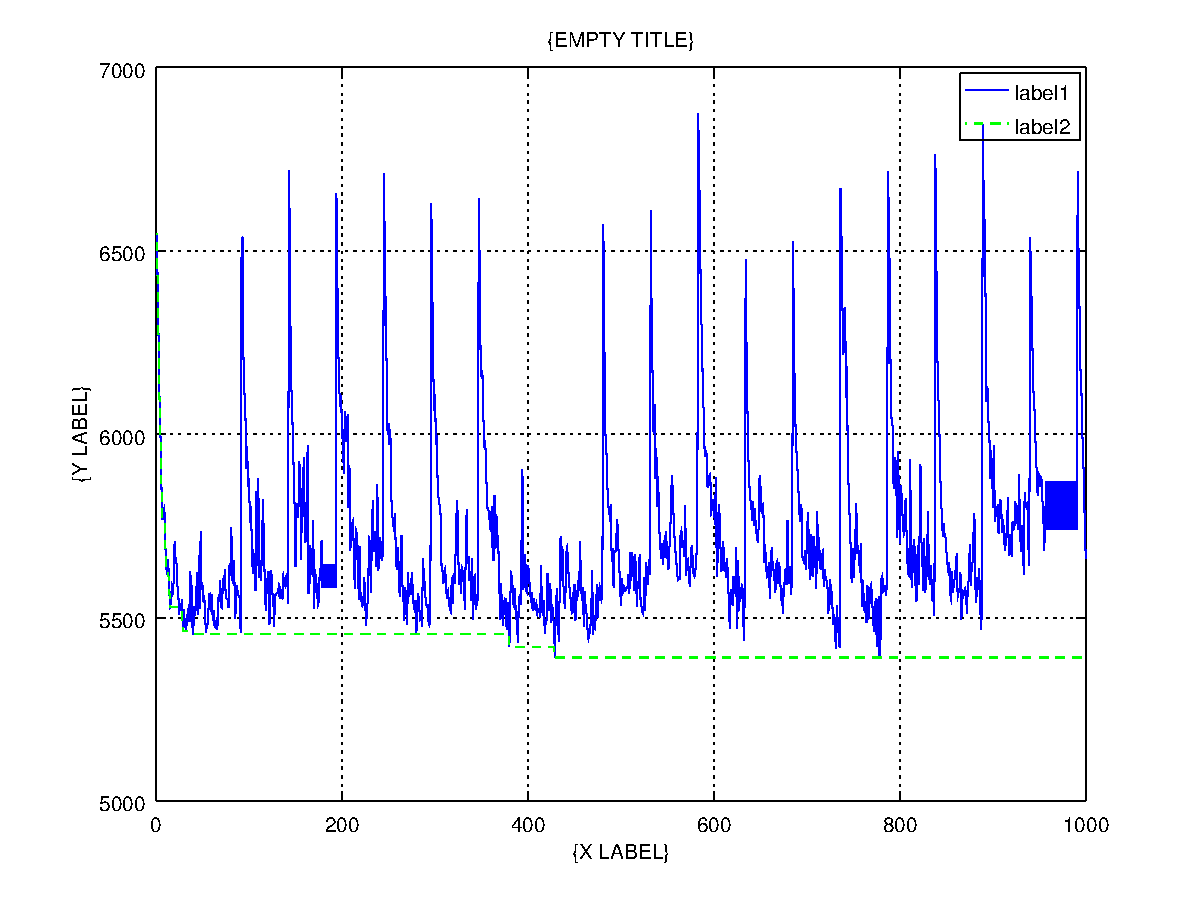
\includegraphics[width=0.67\textwidth]{Appendix_I/GENERATE-PLOT-example/1}
	\hfill\null
	\caption{
		Wygenerowany wykres dwóch funkcji dla przykładowego wywołania skryptu \textsc{generatePlot.bash}, obrazujący sposób zachowania się algorytmu \textsc{Tabu Search} dla przykładowej instancji grafu $G = \left( V, E \right)$, gdzie $\left| V \right| = 30$ ($G$ jest grafem pełnym), dla okresu szukania rozwiązania równego $50$ (po którym następuje ,,restart'' algorytmu).
	}
	\label{fig:genplot}
\end{figure}

\section{Możliwości biblioteki}

Tak jak wspomnieliśmy na samym początku tego rozdziału, biblioteka \textsc{RIT} implementuje wiele z, dotąd przez nas poznanych, algorytmów. Aby zaprezentować możliwość ich wykorzystania, przedstawimy kilka przypadków działania aplikacji, gdzie każdym z nich będziemy starali odpowiedzieć się na jedno z podstawowych pytań, jakie mogą się nasunąć podczas zapoznawania się ze strukturą wspomnianej biblioteki. Należy mieć na uwadze, że prezentowane w tej części wycinki kodu źródłowego w charakterze odpowiedzi na każde z zadanych przez nas pytań, nie są odpowiedziami jedynymi słusznymi --- większość obiektów, jakie będziemy prezentować, biblioteka \textsc{RIT} pozwala stworzyć na więcej niż jeden sposób. My zaś będziemy starali się prezentować tylko te przypadki użycia, które naszym zdaniem pojawiać się mogą najczęściej przy korzystaniu z niej.

\subsection{Budowanie grafu}

Podstawową czynnością jaką musimy mieć możliwość wykonać, jest budowa grafu, na którym będziemy mogli operować. 

\subsubsection{W jaki sposób zbudować graf przy wykorzystaniu udostępnionych funkcji?}

Biblioteka \textsc{RIT} zapewnia kilka sposobów na generowanie grafów, dla których będziemy później chcieli wykonywać obliczenia. Główne z nich to:
\begin{itemize}
	\item odczytanie definicji całego grafu z pliku --- główne z obsługiwanych formatów opiszemy poniżej, na tę chwilę jesteśmy zainteresowani tylko sposobem wywołania danej funkcjonalności\footnote{W prezentowanych przypadkach użycia pomijamy obsługę wyjątków, zgłaszanych w czasie wykonywania programu, przykładowo prezentując sposób ich przechwytywania tylko w pierwszym z nich.}:
	
	\begin{minted}[escapeinside=||,mathescape=true,linenos=true,fontsize=\footnotesize]{c++}
#include <IMST/exp/IOExceptions.hpp>
#include <IMST/utils/enums/InputFormat.hpp>
#include <IMST/utils/enums/InputMode.hpp>
#include <IMST/utils/IOUtils.hpp>
#include <IMST/utils/MemoryUtils.hpp>

int main() {
	GraphIF* g { };
	try {
		g = InputUtils::readGraph("ścieżka do pliku *.gr", InputFormat::GR, InputMode::HDD);
		MemoryUtils::removeGraph(g, true, true);
	} catch (IOExceptions::FileNotFountException& e) {
		return 0;
	}
	return 0;
}
	\end{minted}
	
	gdzie wartość enumerowana \mintinline{C++}|InputFormat| odpowiada za format, który zdecydowaliśmy się wczytać do programu, \mintinline{C++}|InputMode| --- za sposób jego załadowania, gdzie \mintinline{C++}|HDD| odpowiada standardowej metodzie odczytu pliku, której będziemy używać. Należy oczywiście pamiętać o usunięciu przed chwilą stworzonego grafu najwcześniej jak to tylko możliwe, jeżeli chcemy ustrzec się przed późniejszymi problemami związanymi z zarządzaniem pamięcią przez program (każdy prezentowany przykład będzie zawierać również kod usuwający stworzone przez siebie obiekty).
	
	\item dynamiczna konstrukcja grafu --- umożliwia stworzenie dowolnej struktury grafowej przy wykorzystaniu metod udostępnianych przez bibliotekę. Poniżej widoczny przykład przedstawia sposób stworzenia grafu z trzema wierzchołkami, gdzie każdy z nich jest połączony z pozostałymi (graf pełny). Dla danej klasy \mintinline{C++}|GraphIF|, podobnie jak dla zdecydowanej większości obiektów, które będziemy wykorzystywać w prezentowanych kodach, jest dostępna większa liczba konstruktorów --- sposób generowania grafu dla każdego z nich różni się od poniższego. W tym konkretnym przypadku graf jest budowany na podstawie dwóch zbiorów danych: jego wierzchołków $V$ oraz, łączących je, krawędzi $E$. Poniżej prezentowany sposób konstrukcji grafu $G = \left( V, E \right)$ jest zatem naturalny:
	
	\begin{minted}[escapeinside=||,mathescape=true,linenos=true,fontsize=\footnotesize]{c++}
VertexSetIF* vSet = new VertexSetImpl { 3 };
EdgeSetIF* eSet = new EdgeSetImpl { 3 };
GraphIF* g = new GraphImpl { vSet, eSet };

for (unsigned int idx = 0; idx < 3; idx += 1) {
	vSet->push_back(new VertexImpl { idx });
}

for (unsigned int idx = 0; idx < 3; idx += 1) {
	eSet->push_back(
		new EdgeImpl { idx, VertexPair(vSet->getElementAt(idx),
			vSet->getElementAt((idx + 1) % 3)), (EdgeCost) idx });
}
MemoryUtils::removeGraph(g, true, true);
	\end{minted}
	gdzie kolejno stworzyliśmy trzy wierzchołki grafu, później zaś, z wykorzystaniem operacji wyznaczania reszty z dzielenia,  jego krawędzie: $e_{01}$, $e_{12}$ oraz $e_{20}$, każda o koszcie \mintinline{C++}|idx|.\\
	
	\item losowe generowanie struktury --- udostępnione przez klasę pomocniczą \mintinline{C++}|GraphUtils| funkcje, umożliwiają między innymi wygenerowanie losowego grafu na podstawie takich danych jak:
	\begin{itemize}
		\item liczba wierzchołków docelowego grafu,
		\item liczba krawędzi / gęstość grafu (jeden z dwóch),
		\item najniższy możliwy koszt łuku,
		\item największa waga jaką może przyjąć krawędź.
	\end{itemize}

	\begin{minted}[escapeinside=||,mathescape=true,linenos=true,fontsize=\footnotesize]{c++}
GraphIF* g = GraphUtils::getRandomGraph(10,0.5,10,15);
MemoryUtils::removeGraph(g, true, true);
	\end{minted}
	gdzie parametrami w tym przypadku są: liczba krawędzi oraz gęstość grafu. Powyższy fragment kodu został wykorzystany do wygenerowania wszystkich instancji grafów, dla których zostały przeprowadzone eksperymenty w rozdziale \ref{ch:exp}.
	
\end{itemize}




\subsubsection{Jakie formaty wejściowe obsługuje biblioteka?}

\subsection{Eksport i wizualizacja rozwiązań}

\subsubsection{Jak zapisać wygenerowany graf?}

\subsubsection{Jak stworzyć dwuwymiarowy model grafu?}

\subsection{Rozwiązywanie problemów grafowych}

\subsubsection{MST?}


Uruchomienie procesu poszukiwania minimalnego drzewa rozpinajacego dla grafu G wymaga od nas wpierw stworzenia instacji solvera, którym będziemy dane zagadnienie rozwiązywać:


gdzie obiekty takie jak są definiowane przed odpowiednie im instrukcje preprocesora w plikach nagłówkowych --- taka modularna budowa biblioteki RIT umożliwia szybką zmianę implementacji praktycznie dowolnej struktury, która jest wykorzystywana w aplikacji, bez potrzeby jej przebudowywania (w takiej sytuacji od użytkownika wymaga się jedynie podmiany odpowiedniego pliku nagłówkowego, który został przez niego zmieniony). 

\subsubsection{ILOG CPLEX?}

\subsubsection{IMST?}

\subsubsection{ILOG CPLEX?}

\subsubsection{AIMST?}

\subsubsection{RRIMST?}


% OS path %%%%%%%%%%%%%%%%%%%%%%%%%%%%%%%%%%%%%%%%%%%%%%%%%%%%%%%%%%%%%%%%%%%%%%%%%%%%%%%%%%%%%%%%%%%%%%%%%%%%%%%%%%
 \textsf{/Scripts/compileProject.bash}

% Shortcut %%%%%%%%%%%%%%%%%%%%%%%%%%%%%%%%%%%%%%%%%%%%%%%%%%%%%%%%%%%%%%%%%%%%%%%%%%%%%%%%%%%%%%%%%%%%%%%%%%%%%%%%%%
 \texttt{CRTL + ALT + T}

% Nazwy własne, argumenty %%%%%%%%%%%%%%%%%%%%%%%%%%%%%%%%%%%%%%%%%%%%%%%%%%%%%%%%%%%%%%%%%%%%%%%%%%%%%%%%%%%%%%%%%%%%%%%%%%%%%%%%%%
\textsc{R\_USATest\_DKA}

% ANG %%%%%%%%%%%%%%%%%%%%%%%%%%%%%%%%%%%%%%%%%%%%%%%%%%%%%%%%%%%%%%%%%%%%%%%%%%%%%%%%%%%%%%%%%%%%%%%%%%%%%%%%%%
(ang. \textit{Directed acyclic graph})

% Figura %%%%%%%%%%%%%%%%%%%%%%%%%%%%%%%%%%%%%%%%%%%%%%%%%%%%%%%%%%%%%%%%%%%%%%%%%%%%%%%%%%%%%%%%%%%%%%%%%%%%%%%%%%

\begin{figure}[!htbp]
	\null\hfill
	%\includegraphics[width=0.8\textwidth]{Appendix_I/GENERATE-PLOT-bash/a_psfrag.pdf}
	\hfill\null
	\caption{
		Wygenerowany wykres dwóch funkcji dla przykładowego wywołania skryptu \textsc{generatePlot.bash}.
	}
\end{figure}

% Figury %%%%%%%%%%%%%%%%%%%%%%%%%%%%%%%%%%%%%%%%%%%%%%%%%%%%%%%%%%%%%%%%%%%%%%%%%%%%%%%%%%%%%%%%%%%%%%%%%%%%%%%%%%

\begin{figure}[!htbp]
	\null\hfill
	\begin{subfigure}[b]{0.49\textwidth}
		\footnotesize
		\begin{lstlisting}[language=bash]
digraph G {
	rankdir=LR;
	node [shape = circle];
	1 -> 2 [ label = "2"];
	1 -> 3 [ label = "6"];
	2 -> 3 [ label = "3"];
	2 -> 4 [ label = "4"];
	2 -> 5 [ label = "5"];
	3 -> 5 [ label = "1"];
	5 -> 4 [ label = "2"];
}
		\end{lstlisting}
		\caption{}
		\label{fig:graphViz:a}
	\end{subfigure}
	\hfill
	\begin{subfigure}[b]{0.49\textwidth}
		%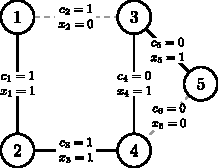
\includegraphics[width=\textwidth]{Appendix_I/GRAPH-VIZ-Example/a.pdf}
		\vspace{1em}
		\caption{}
		\label{fig:graphViz:b}
	\end{subfigure}
	\hfill\null
	\caption{
		Wygenerowana ilustracja grafu przez skrypt \textsc{makeGraphViz.bash}.
		\textbf{(a)}~Kod pośredni pomiędzy danymi wejściowymi w standardowym formacie \textsc{DIMACS Implementation Challenge} a finalnym rysunkiem. Kod pośredni jest zapisany w języku \textsc{DOT}.
		\textbf{(b)}~Rysunek grafu wygenerowany przez program \textsc{GraphViz}.
	}
	\label{fig:graphViz}
\end{figure}

% URL %%%%%%%%%%%%%%%%%%%%%%%%%%%%%%%%%%%%%%%%%%%%%%%%%%%%%%%%%%%%%%%%%%%%%%%%%%%%%%%%%%%%%%%%%%%%%%%%%%%%%%%%%%

\url{http://algs4.cs.princeton.edu/home/} na licencji \textsc{GNU GPLv3}

% ALIGN %%%%%%%%%%%%%%%%%%%%%%%%%%%%%%%%%%%%%%%%%%%%%%%%%%%%%%%%%%%%%%%%%%%%%%%%%%%%%%%%%%%%%%%%%%%%%%%%%%%%%%%%%%

	\begin{align*}
		f(x) +    g(x)  &=          \cos(x) +              \sin(x)             + h(x) \\
		\phantom{f(x) +{}} g(x)  &= \phantom{\cos(x) +{}}          {\sin(x)} \phantom{{}+ h(x)}\\
		f(x)  \phantom{{}+ g(x)} &=          \cos(x) \phantom{{} +  \sin(x)}            + h(x) \\
		s(x)  \phantom{{}+ g(x)} &= \phantom{\cos(x) +{}} \makebox[\widthof{$\sin(x) + h(x)$}][c]{$\arcsin(x)$}
	\end{align*}
	\clearpage

\end{document}